% Who is at the keyboard? Process-Aware Authorship Continuity in Programming Assessment
% M.Tech thesis, IIIT Surat. Build: latexmk -pdf main.tex
\documentclass[12pt,a4paper,oneside]{report}

% ---------- Thesis metadata (used by the title page) ----------
\newcommand{\thesistitle}{Who is at the Keyboard?\\[0.3em]
  \large Process-Aware Authorship Continuity in Programming Assessment}
\newcommand{\thesistitleplain}{Who is at the Keyboard? Process-Aware Authorship Continuity in Programming Assessment}
\newcommand{\authorname}{Rohandeep}
\newcommand{\rollno}{PG25CS07}
\newcommand{\degree}{Master of Technology}
\newcommand{\branch}{Computer Science and Engineering}
\newcommand{\supervisor}{Dr.\ Ritesh Kumar}
\newcommand{\department}{Department of Computer Science and Engineering}
\newcommand{\institute}{Indian Institute of Information Technology Surat}
\newcommand{\submissionyear}{2027}

% ---------- Layout ----------
\usepackage[a4paper,left=1.5in,right=1in,top=1in,bottom=1in]{geometry}
\usepackage{setspace}
\onehalfspacing
\usepackage[T1]{fontenc}
\usepackage[utf8]{inputenc}
\usepackage{lmodern}
\usepackage{microtype}

% ---------- Maths, tables, figures ----------
\usepackage{amsmath,amssymb,amsthm}
\usepackage{graphicx}
\graphicspath{{figures/}{snapshots/}{graphs/}{flowcharts/}}
\usepackage{booktabs,multirow,tabularx}
\usepackage{siunitx}
\usepackage{float}
\usepackage{caption,subcaption}
\usepackage{xcolor}
\usepackage{tikz}
\usetikzlibrary{arrows.meta,positioning,shapes.geometric,fit,calc,backgrounds}
\usepackage{pgfplots}
\pgfplotsset{compat=1.17}
\usepackage{listings}
\lstset{basicstyle=\ttfamily\small,breaklines=true,frame=single}
\usepackage{enumitem}

% ---------- References ----------
\usepackage[backend=biber,style=ieee,sorting=none]{biblatex}
\addbibresource{bib/references.bib}
\usepackage[hidelinks]{hyperref}
\usepackage[nameinlink,capitalise]{cleveref}

% ---------- Helpers ----------
\newtheorem{definition}{Definition}[chapter]
% Visible drafting note; remove before submission.
\newcommand{\todo}[1]{\textcolor{red}{[TODO: #1]}}
% Pull in a figure from flowcharts/*.tex (TikZ)
\newcommand{\tikzfig}[1]{\input{flowcharts/#1}}
\newcommand{\RQ}[1]{\textbf{RQ#1}}


\begin{document}

% ---------- Front matter ----------
\pagenumbering{roman}
% Replace with the official IIIT Surat title page once the template is available.
\begin{titlepage}
  \centering
  {\LARGE\bfseries \thesistitle\par}
  \vspace{1.5cm}
  {\large A thesis submitted in partial fulfilment of the requirements\\
  for the award of the degree of\par}
  \vspace{0.5cm}
  {\Large\bfseries \degree\par}
  {\large in\par}
  {\Large \branch\par}
  \vspace{1.5cm}
  {\large by\par}
  \vspace{0.3cm}
  {\Large\bfseries \authorname\par}
  {\large (\rollno)\par}
  \vspace{1.5cm}
  {\large Under the supervision of\par}
  {\Large \supervisor\par}
  \vfill
  % \includegraphics[width=3cm]{figures/iiit-surat-logo}\par\vspace{0.5cm}
  {\large \department\par}
  {\large\bfseries \institute\par}
  {\large \submissionyear\par}
\end{titlepage}

\chapter*{Certificate}
\addcontentsline{toc}{chapter}{Certificate}

This is to certify that the thesis entitled \textbf{``\thesistitleplain''},
submitted by \textbf{\authorname} (\rollno) to the \institute{} in partial
fulfilment of the requirements for the award of the degree of
\textbf{\degree} in \branch, is a bona fide record of research work carried
out under my supervision. The contents of this thesis have not been
submitted elsewhere for the award of any degree or diploma.

\vspace{2.5cm}
\noindent
\begin{tabular}{@{}l}
\supervisor \\
Supervisor \\
\department \\
\institute
\end{tabular}

\chapter*{Declaration}
\addcontentsline{toc}{chapter}{Declaration}

I declare that this thesis represents my ideas in my own words, and where
others' ideas or words have been included, I have adequately cited and
referenced the original sources. I also declare that I have adhered to all
principles of academic honesty and integrity and have not misrepresented,
fabricated or falsified any idea, data, fact or source in my submission.

\vspace{2.5cm}
\noindent
\begin{tabular}{@{}l}
\authorname{} (\rollno) \\
Date:
\end{tabular}

\chapter*{Acknowledgements}
\addcontentsline{toc}{chapter}{Acknowledgements}

\todo{Thank the supervisor, study participants, lab staff, ethics committee.}

\chapter*{Abstract}
\addcontentsline{toc}{chapter}{Abstract}

% Draft from the mid-semester presentation; rewrite once results exist.
Programming assessments check who a student is at the start of a session,
and whether the submitted code was copied or generated at the end. Nothing
checks that the same person kept writing in between. This thesis studies
\emph{authorship continuity}: detecting when a different person, such as a
friend or a paid proxy, takes over partway through a coding session. We
build the Student IDE, a lab code editor that records keystroke timing,
pastes, edits and code runs without any webcam or screen recording. From
each student's first four weeks of labs we learn a personal baseline of
coding habits, score every 30-second window against it, and use a CUSUM
change-point detector to flag a likely takeover and estimate when it
happened. Teachers see an evidence timeline, and a flag leads only to a
conversation, never a penalty. \todo{Headline results for RQ1--RQ4.}

\vspace{1em}
\noindent\textbf{Keywords:} keystroke dynamics, authorship continuity,
change-point detection, CUSUM, programming education, academic integrity.


\tableofcontents
\listoffigures
\listoftables
\chapter*{Abbreviations}
\addcontentsline{toc}{chapter}{Abbreviations}

\begin{tabular}{@{}ll}
AST   & Abstract Syntax Tree \\
CUSUM & Cumulative Sum (change-point detection) \\
DPDP  & Digital Personal Data Protection (Act, India, 2023) \\
EER   & Equal Error Rate \\
IAT   & Inter-key (inter-arrival) Time \\
IDE   & Integrated Development Environment \\
RQ    & Research Question \\
\end{tabular}


% ---------- Main matter ----------
\cleardoublepage
\pagenumbering{arabic}

\chapter{Introduction}
\label{ch:intro}

\section{Motivation}
Programming assessments increasingly happen on a computer, in a lab or
remotely. Identity is checked when a session starts, and the final code is
checked for copying or generated text when it ends. A student can pass both
checks while somebody else wrote most of the code: a friend who takes the
keyboard for twenty minutes, or a paid proxy on a remote call.
\todo{Evidence of the problem: contract cheating / proxy statistics.}

\section{Authorship continuity}
\begin{definition}[Authorship continuity]
A coding session has authorship continuity if the same person produced all
of its keystrokes and edits.
\end{definition}
This thesis asks whether a break in continuity can be detected from how
code is written (process), without watching the student.

\section{Research questions}
\begin{description}[leftmargin=2.5em]
  \item[\RQ{1}] Can a mid-session change of author be detected, and how
    quickly and with how many false alarms? \emph{(main contribution)}
  \item[\RQ{2}] Can composing original code be distinguished from
    transcribing code from another source?
  \item[\RQ{3}] Does a baseline learned in the lab transfer to a remote
    interview on the student's own laptop?
  \item[\RQ{4}] Is the detector fair across subgroups, and what is its
    precision at realistic cheating rates (1 in 100, 1 in 500)?
\end{description}

\section{Contributions}
\begin{enumerate}
  \item The Student IDE, a privacy-preserving event-logging editor.
  \item Per-student habit baselines over 30-second windows.
  \item A CUSUM-based switch detector that also estimates the switch time.
  \item A teacher-facing evidence timeline designed so a flag leads to a
    conversation, not a penalty.
  \item A staged-takeover dataset and evaluation with fairness and
    prevalence-adjusted precision.
\end{enumerate}

\section{Thesis outline}
\todo{One line per chapter once chapters stabilise.}

\chapter{Background and Related Work}
\label{ch:background}

\section{Keystroke dynamics}
Fixed-text and free-text keystroke biometrics \cite{monrose2000keystroke},
benchmark of anomaly detectors including scaled Manhattan
\cite{killourhy2009comparing}, and deep free-text models such as TypeNet
\cite{acien2022typenet}.

\section{Keystroke data in programming education}
Programmer identification from typing \cite{longi2015identification}.
In essay writing, keystroke-process features separate original composition
from transcription with high accuracy, because transcription is more linear
and bursty \cite{crossley2024plagiarism}.

\subsection{Nosi IDE: the closest prior work}
Nosi \cite{lueder2026nosi} is a fork of VS Code with LLM features disabled.
Assignments are distributed as encrypted files that are decrypted only in
memory, so copying code out produces an encrypted payload and every paste
is logged with its timestamp and content. This leaves manual retyping
(``scribing'') of LLM output as the remaining stealthy route, which Nosi
targets with one feature: the L-scale (an L-moment measure of dispersion)
of log-transformed inter-arrival times (IAT) between keystrokes, after
removing pauses over 5 minutes and zero-length intervals. Authentic coding
has a long-tailed IAT distribution; scribing is flatter.

The evidence is a proof-of-concept with $N = 5$, all authors and proficient
coders, in an A--B--B--A design (code, scribe, scribe, code) on one
priority-queue task. A linear SVM on the single feature reached 100\%
leave-one-participant-out accuracy on whole sessions and about 80\% on
\SI{150}{\second} slices; typing comments was sometimes misread as
scribing. In deployment in a course of about 1000 students, staff found 48
cases of LLM-assisted plagiarism by replaying edit logs.

Nosi differs from this thesis in three ways. It asks whether code was
\emph{transcribed}, not whether the \emph{author changed}; it uses a
population-level, subject-independent classifier rather than a per-student
baseline; and its sample is five expert authors. \RQ{2} replicates its
measure at larger $N$ with ordinary students, and \RQ{1} addresses the
switch it does not model.

\section{Academic integrity tooling}
Identity checks at the start (proctoring), similarity and AI detection at
the end, paste detection. \todo{Survey and position the gap: nothing
checks continuity in between.}

\section{Change-point detection}
CUSUM \cite{page1954continuous} and sequential change detection
\cite{basseville1993detection}.

\section{Privacy, regulation and fairness}
India's DPDP Act \cite{dpdp2023}; EU AI Act high-risk requirements for
education \cite{euaiact2024}. \todo{Fairness in biometric systems.}

\section{Summary of the gap}
\todo{Table: prior work vs.\ start/middle/end coverage, privacy, N.}

\chapter{Problem Formulation}
\label{ch:problem}

\section{Threat model}
In scope: a friend, paid proxy or impersonator takes over for part or all
of a session (full proxy, takeover at a random minute), copying code out of
another source, pasting. Out of scope: deliberate imitation of another
student's typing, deepfakes, engagement scoring, grade prediction,
deployment.

\section{Formal setting}
\todo{Session as a stream of events $e_1, e_2, \dots$; windows of
\SI{30}{\second}; feature vector $x_t$; baseline $B_s$ for student $s$;
score $d_t = d(x_t, B_s)$; switch time $\tau$; detection delay
$\hat\tau - \tau$.}

\section{Research questions and hypotheses}
\todo{Restate RQ1--RQ4 with measurable hypotheses and metrics.}

\section{Design principles}
\begin{itemize}
  \item No webcam or screen recording.
  \item Each student compared only to their own baseline.
  \item Raw keystrokes deleted after the baseline is built; summary
    statistics only.
  \item A flag starts a conversation, never a penalty.
\end{itemize}

\chapter{The Student IDE}
\label{ch:system}

\section{Architecture}
\begin{figure}[ht]
  \centering
  \tikzfig{pipeline}
  \caption{The Student IDE pipeline. Parts 3--5 are the novel contribution.}
  \label{fig:pipeline}
\end{figure}

\section{Event logging editor}
\todo{What is logged (key down/up, paste, edit, cursor, run, error,
snapshot), timing precision, tech stack and why. Screenshot in
\texttt{snapshots/}. Feeds from brain entries tagged 04-system-design.}

\subsection{Student interface}
The student-facing screens (sign-in, consent, task picker, editor, run
output) were redesigned once the logger worked
(\cref{fig:ui-before-after}). The interface is React with Tailwind CSS
and the Motion animation library, on top of a small shared design system
(colour tokens with light and dark themes, motion presets and UI
primitives) that the teacher timeline will reuse.

Motion is deliberately kept away from timing capture. The CodeMirror
editor is created once and never re-rendered, so a keystroke causes no
interface work beyond CodeMirror's own; animations run only on discrete
actions (a run finishing, the finish dialog) and touch only opacity and
transform so the browser can composite them off the main thread; and key
times are taken from the browser event timestamp, not from when a handler
runs. The end-to-end test confirms the event stream is unchanged
(214 events of the same types before and after) and asserts that no main
thread task longer than \SI{50}{\milli\second} overlaps the typing window.
The consent text is unchanged; the motion respects the operating system's
reduced-motion setting.

\begin{figure}[ht]
  \centering
  \begin{subfigure}{0.48\textwidth}
    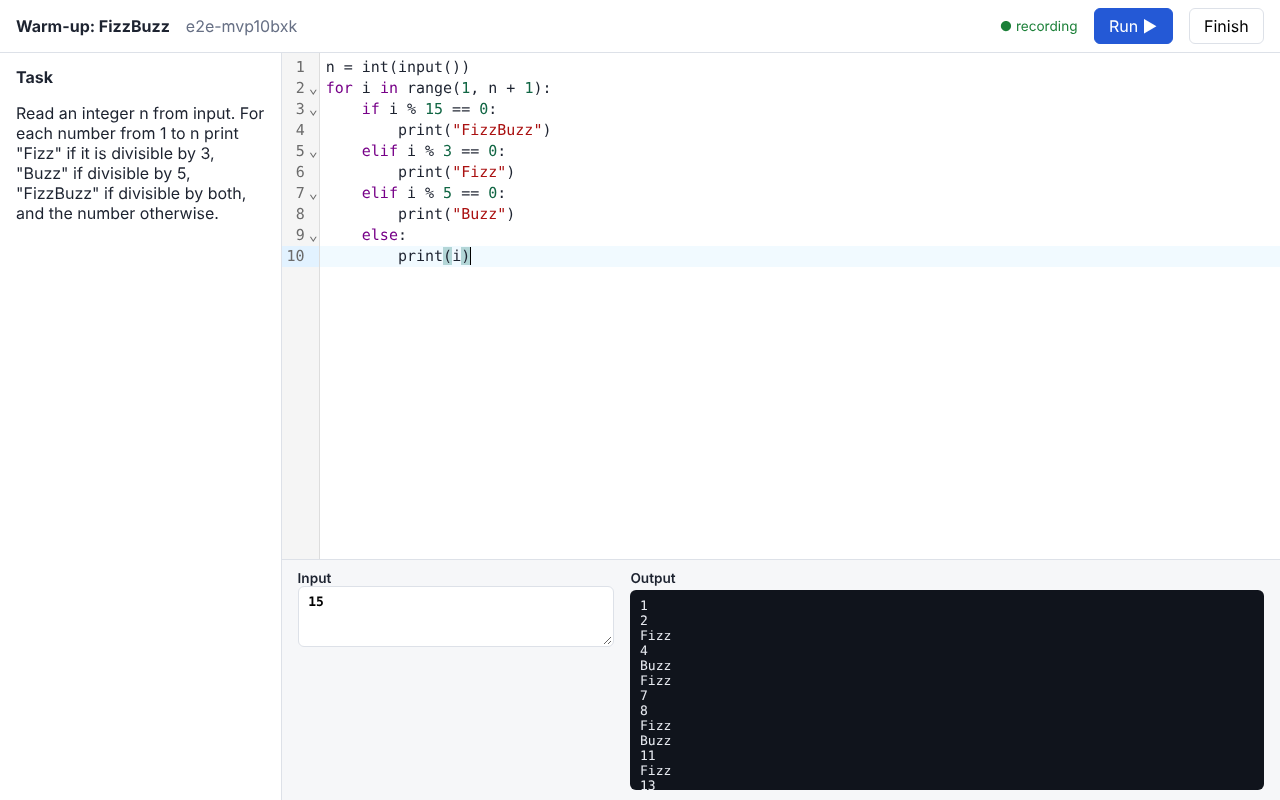
\includegraphics[width=\linewidth]{ui-redesign/before-04-editor}
    \caption{Phase 1 editor}
  \end{subfigure}\hfill
  \begin{subfigure}{0.48\textwidth}
    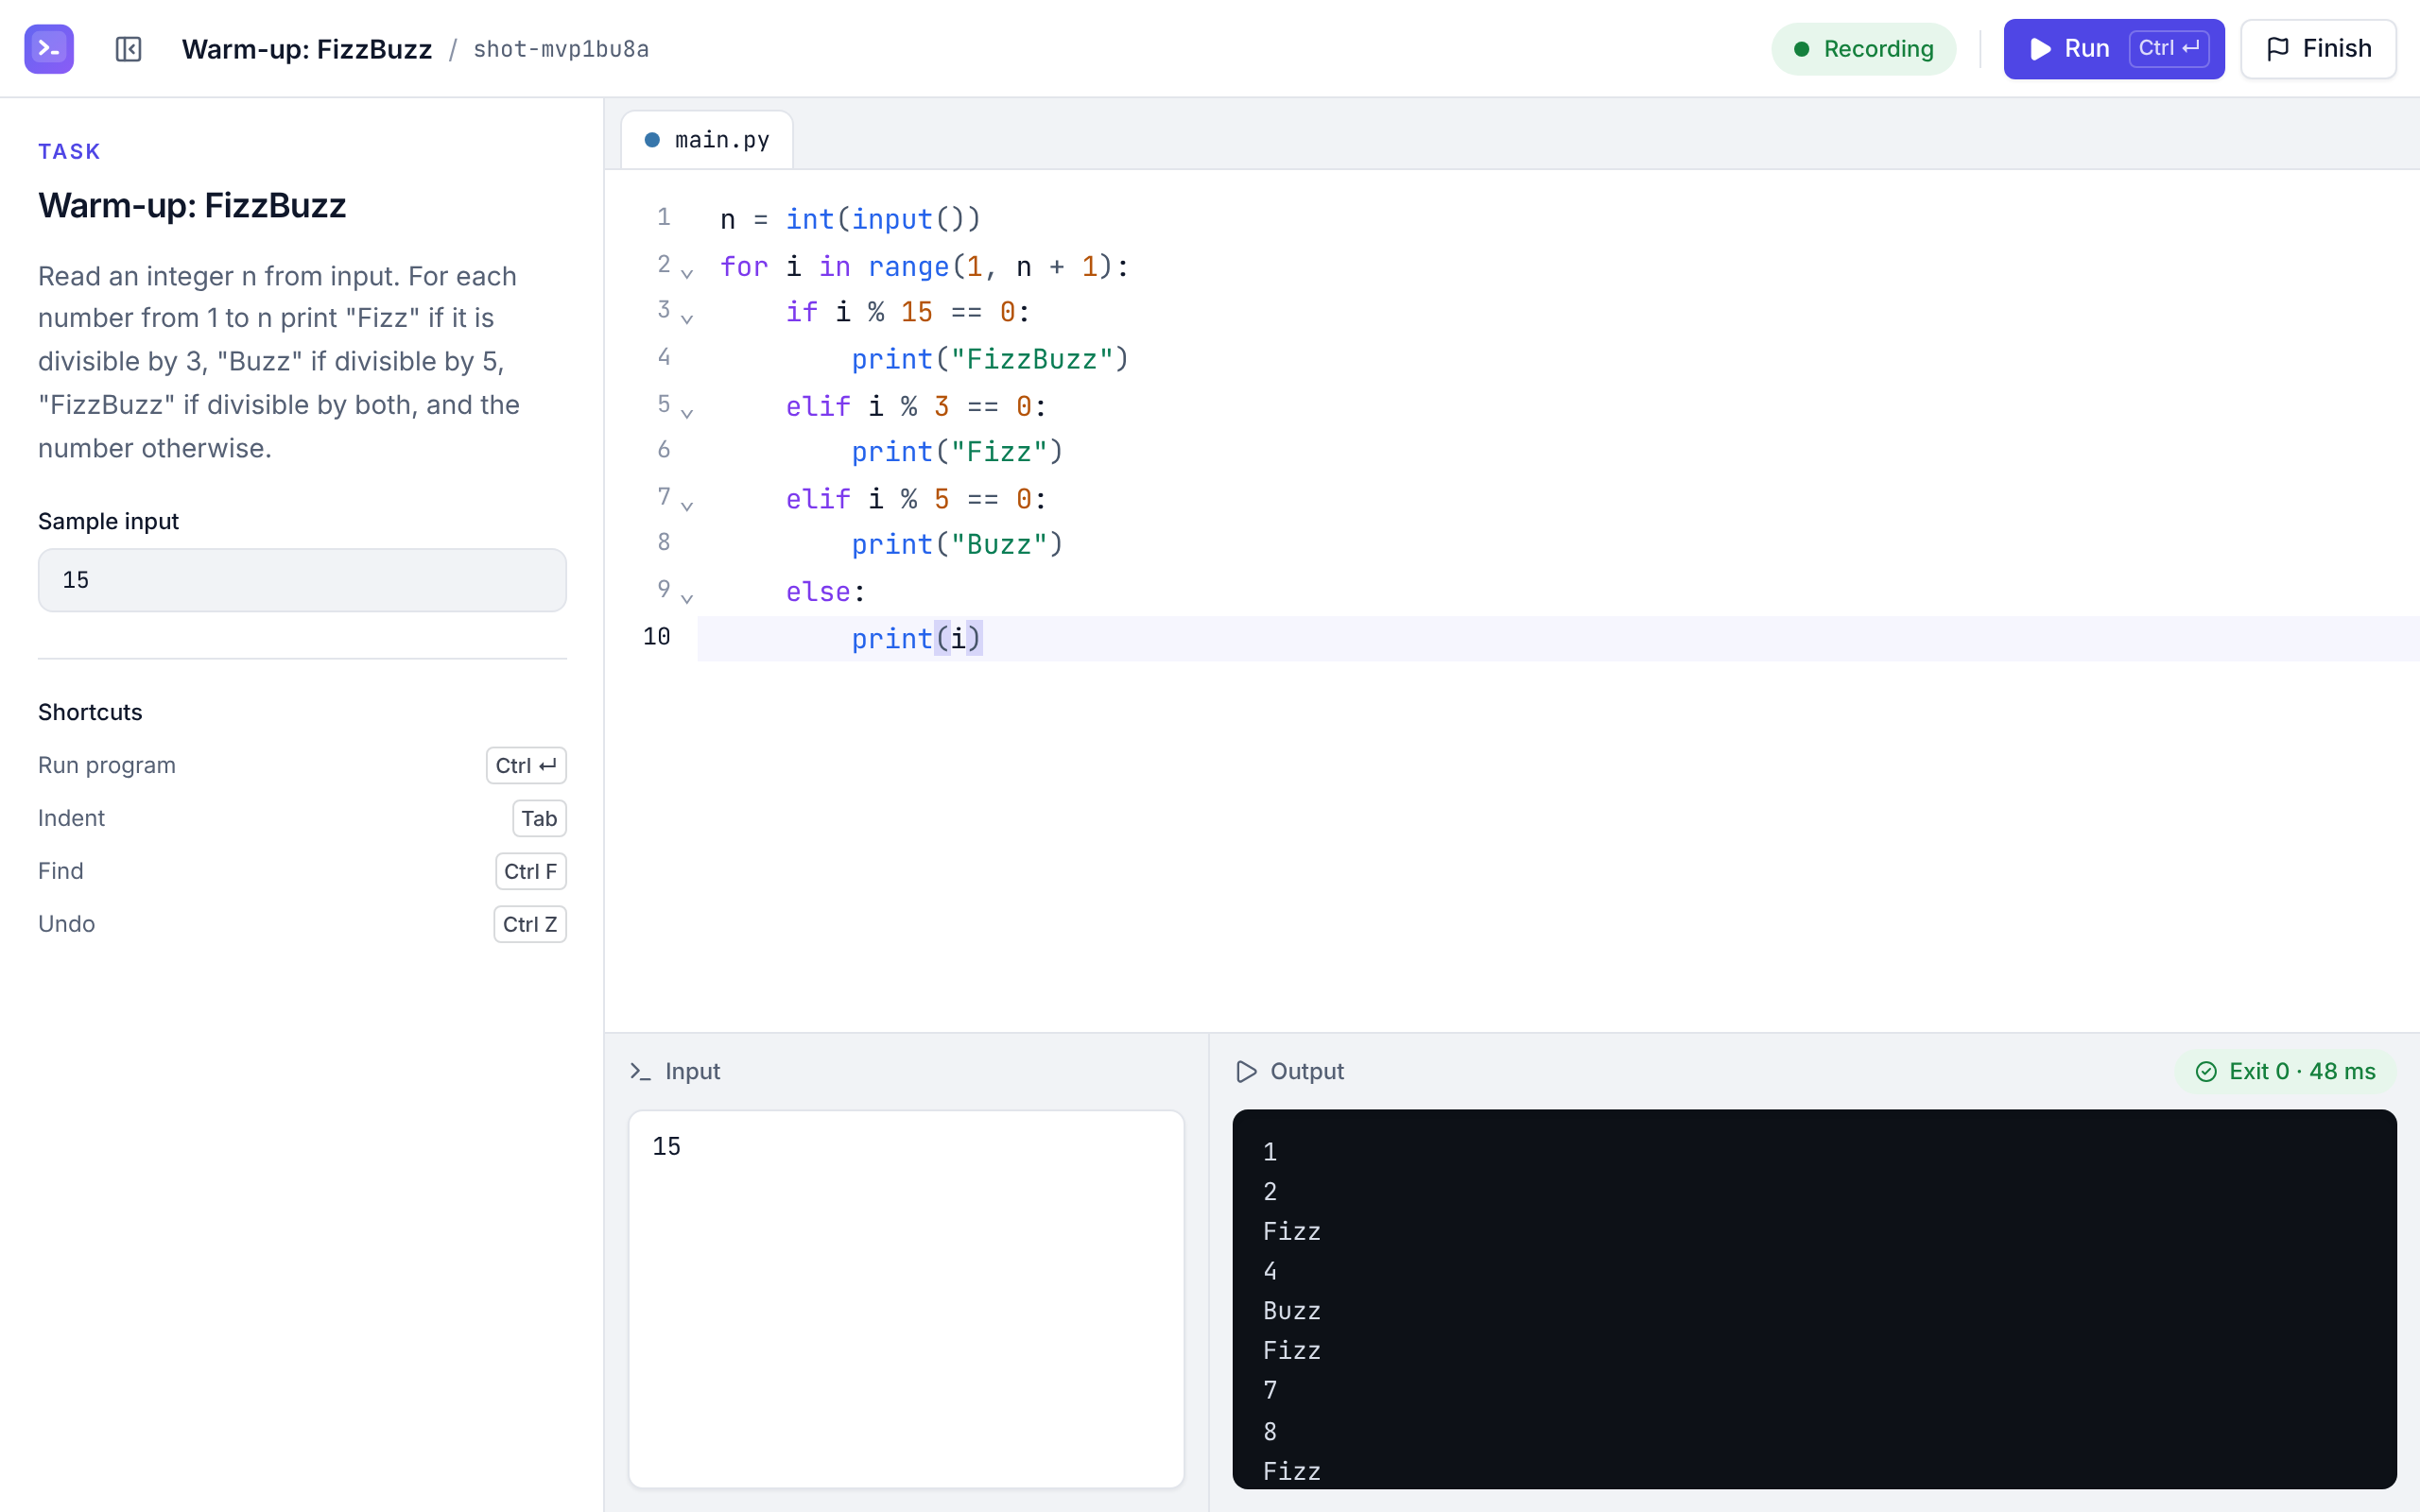
\includegraphics[width=\linewidth]{ui-redesign/after-light-05-run-output}
    \caption{Redesigned editor after a run}
  \end{subfigure}\\[1ex]
  \begin{subfigure}{0.48\textwidth}
    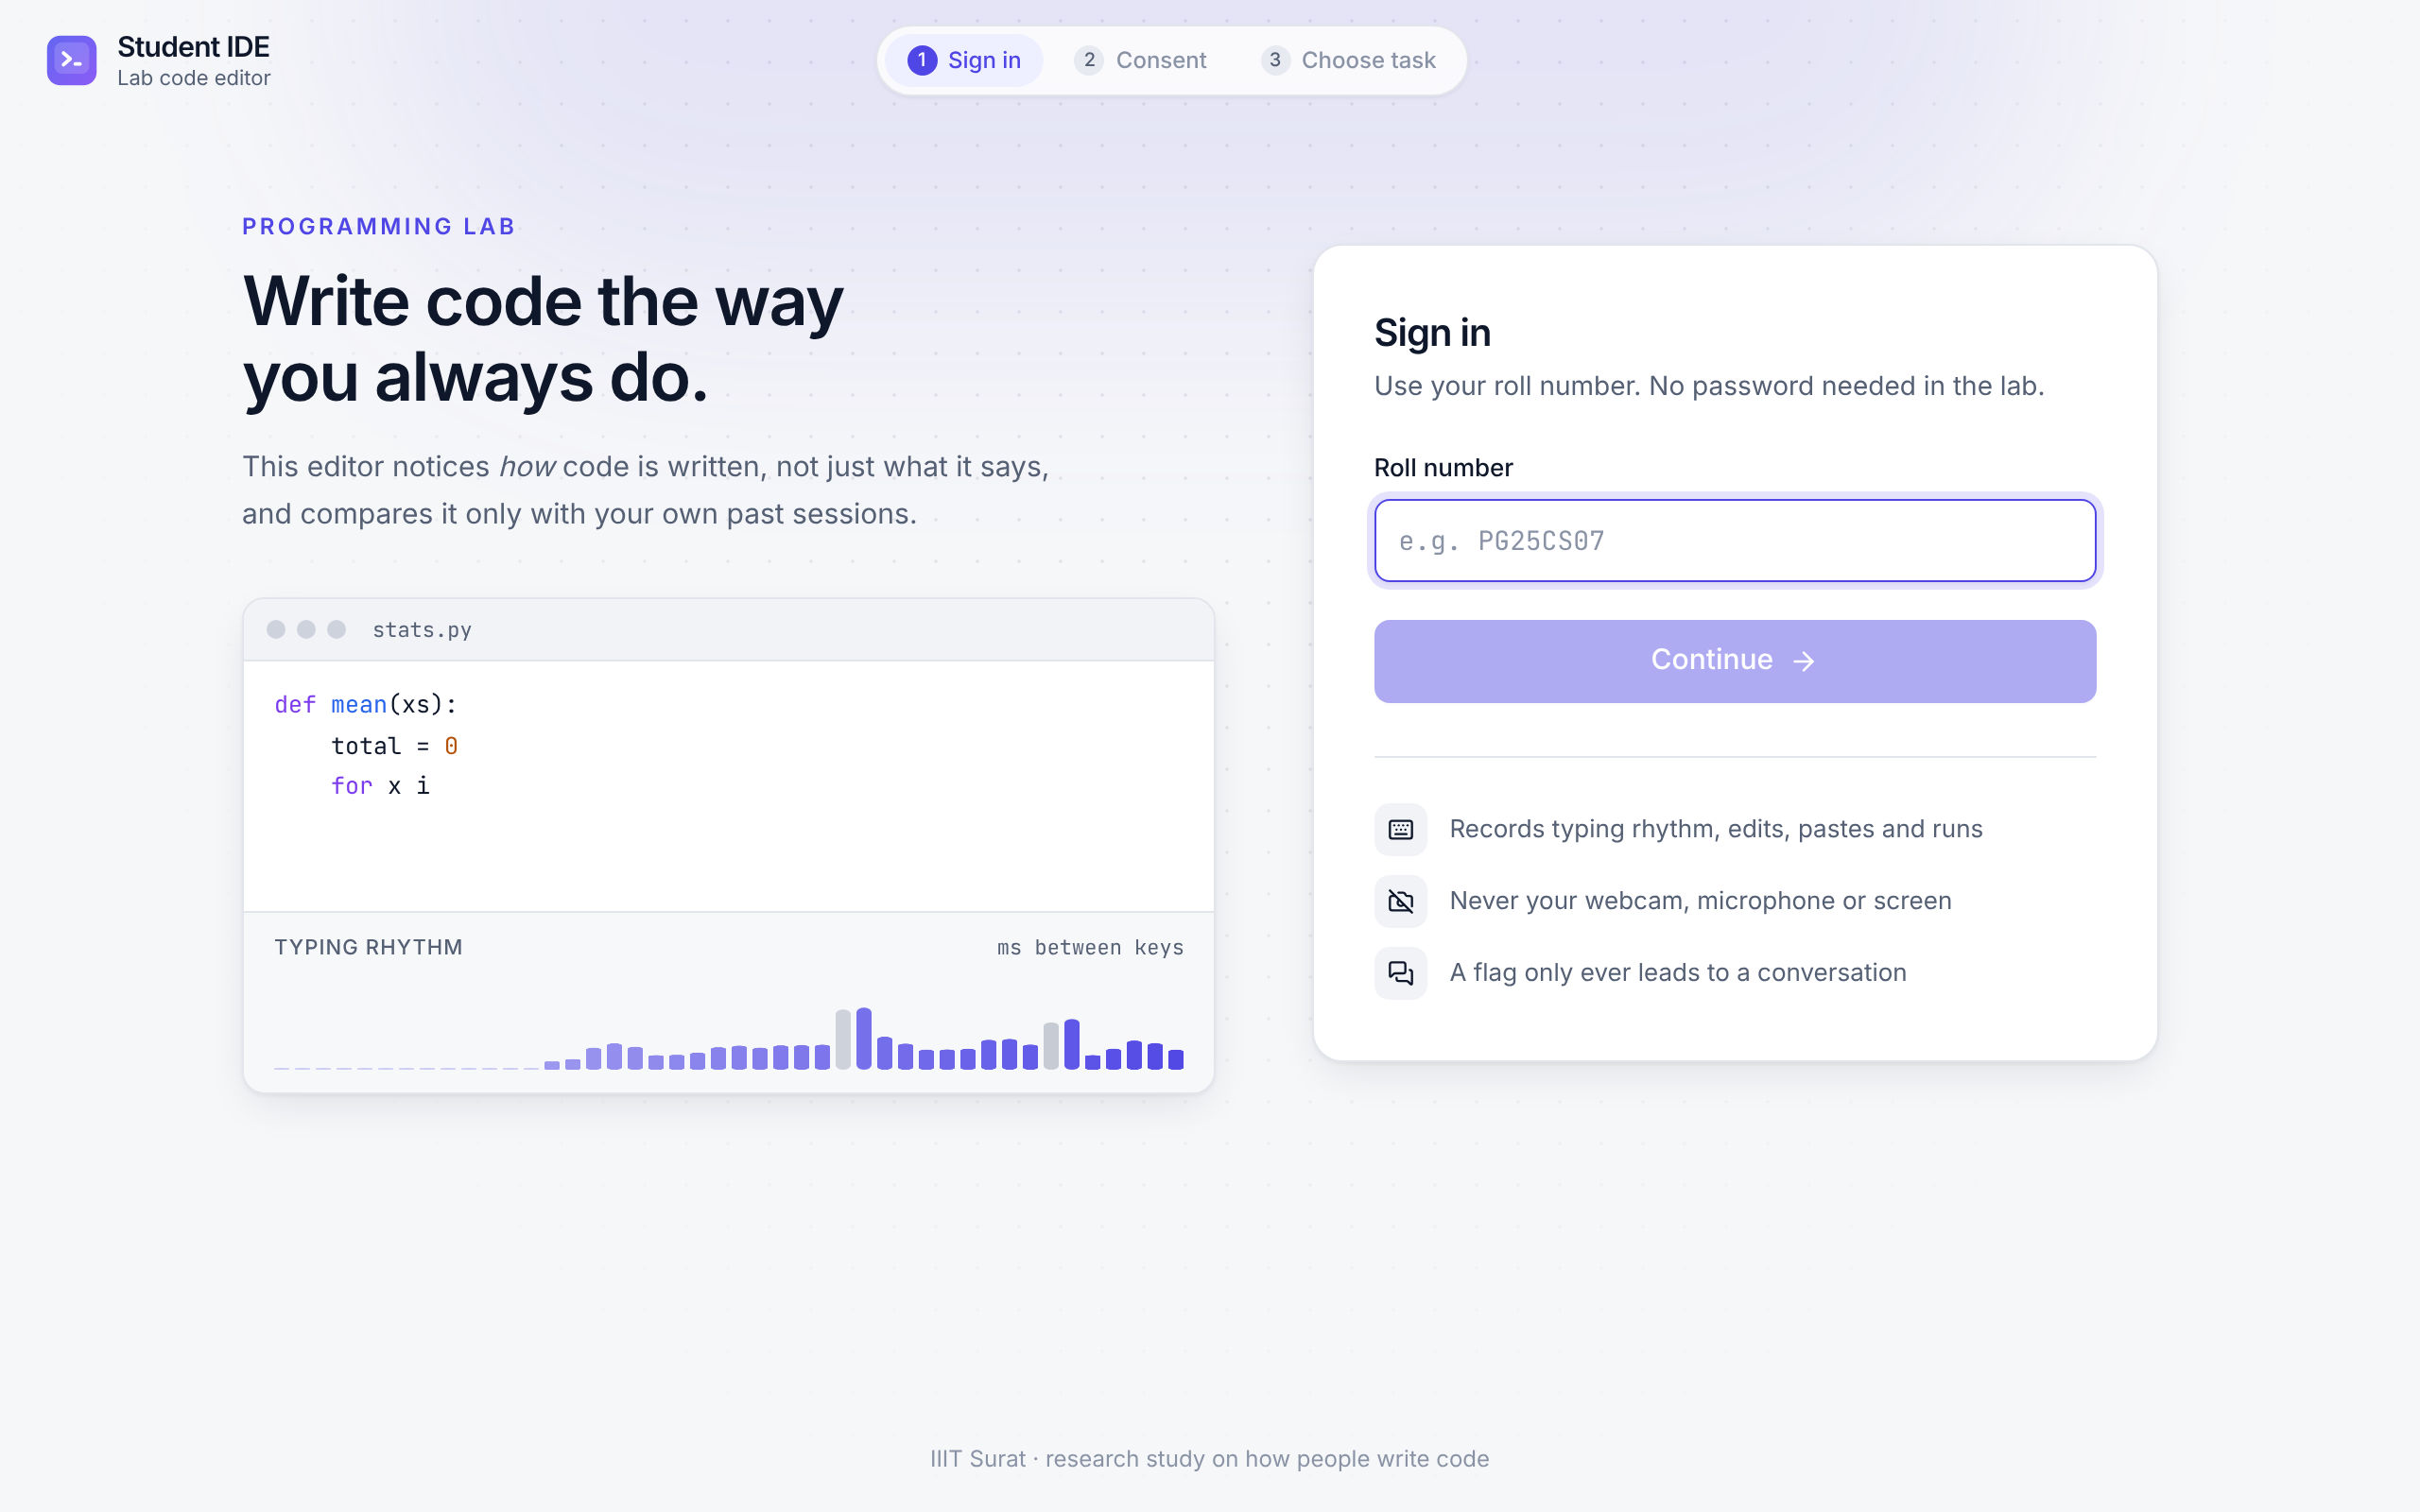
\includegraphics[width=\linewidth]{ui-redesign/after-light-01-login}
    \caption{Sign-in with the keystroke-rhythm illustration}
  \end{subfigure}\hfill
  \begin{subfigure}{0.48\textwidth}
    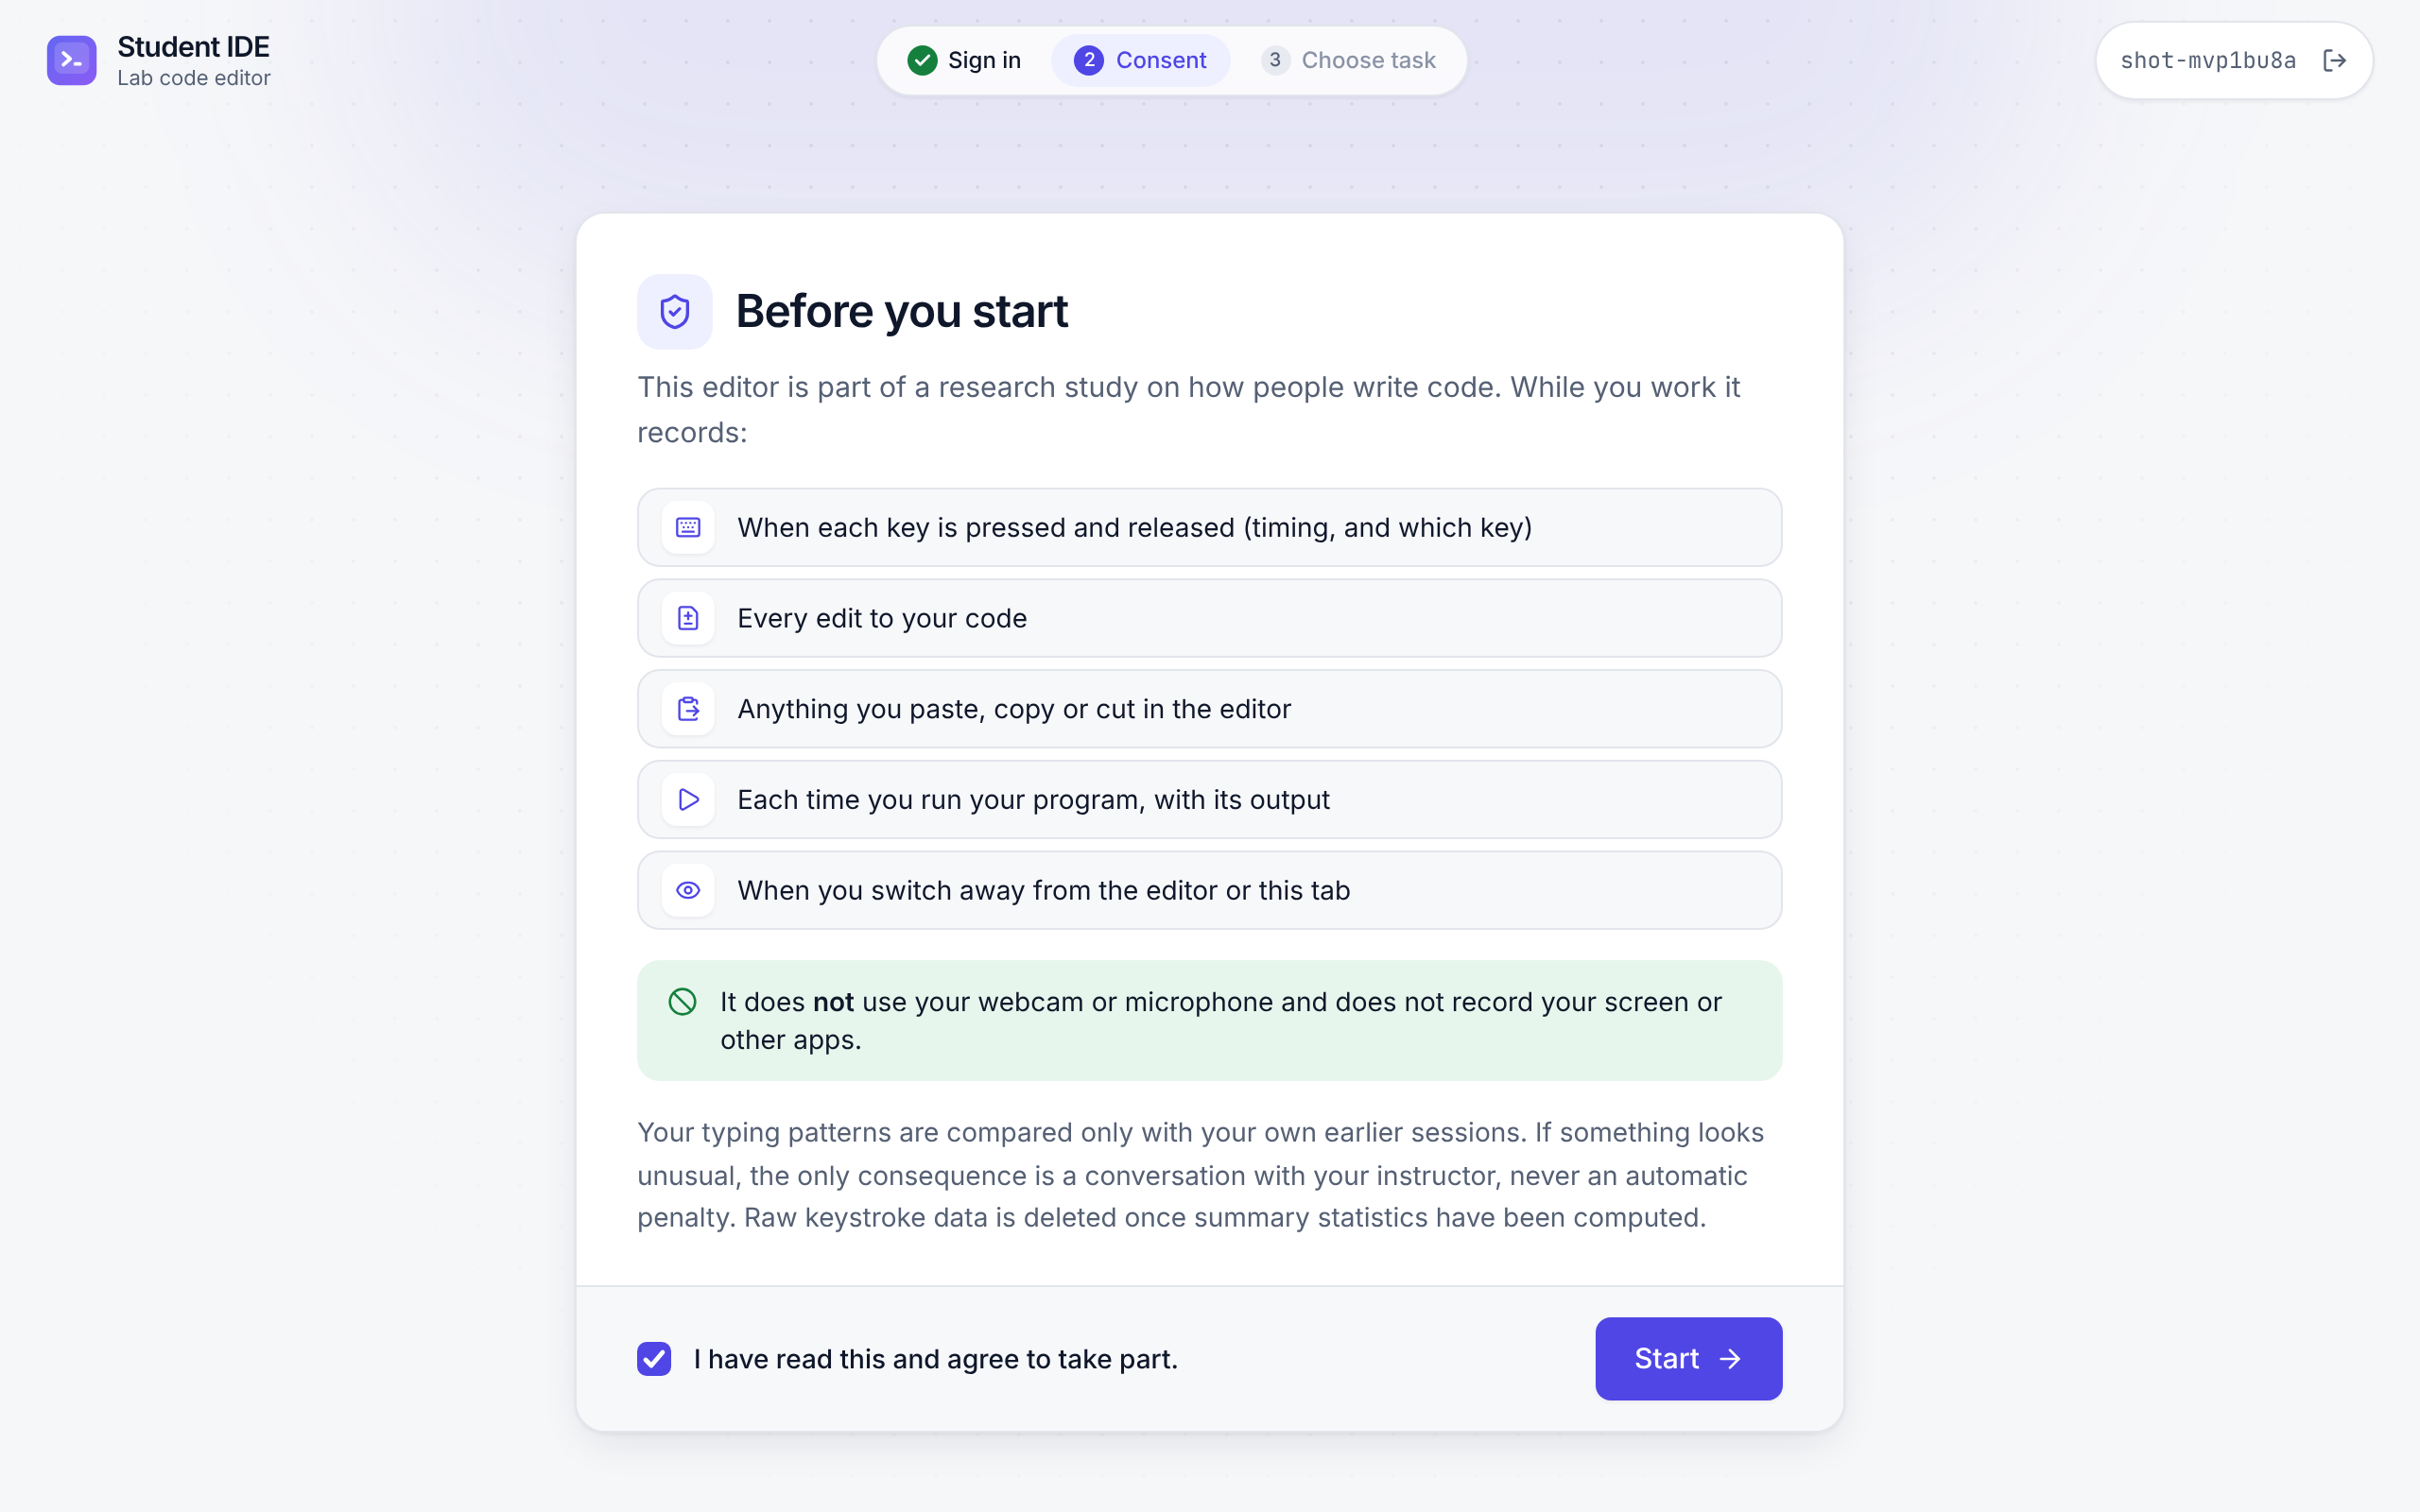
\includegraphics[width=\linewidth]{ui-redesign/after-light-02-consent}
    \caption{Consent notice}
  \end{subfigure}
  \caption{Student interface before and after the redesign. All screens,
  in light and dark themes, are in \texttt{snapshots/ui-redesign/}.}
  \label{fig:ui-before-after}
\end{figure}

\section{Event schema and storage}
\todo{Summary here, full schema in \cref{app:schema}.}

\section{Privacy and data lifecycle}
\todo{Raw keystrokes $\rightarrow$ baseline summary $\rightarrow$
deletion. Retention, consent, DPDP mapping.}

\section{Labs and questions}
\label{sec:teacher-authoring}
Teachers set up the sittings students record in from the same token-gated
area as the review timeline (\cref{fig:teach}). A \emph{lab} is one sitting,
such as a weekly lab class or one of the staged study sessions of
\cref{ch:study}. It holds ordered questions, each with a prompt, optional
starter code that opens in the editor and a sample input, and is assigned to
a roster of roll numbers or to everyone who signs in. A lab is a draft, open
(assigned students see it and can start) or closed (hidden, recordings kept).

Each recorded session stores the lab and question it answers, so every
keystroke, edit and run is tied to them through the session without changing
the event schema. The session also keeps a copy of the question as the
student saw it: a teacher may correct a prompt halfway through a lab, and an
older recording must still say what it was answering, which matters when
composing and transcribing are compared on the same question (RQ2). Labs and
questions with recordings can be closed or edited but not deleted. Because
each staged condition can be its own lab with its own roster, the condition
label of a study recording can come from the lab it was made in rather than
from a separate hand-kept list.

\begin{figure}[ht]
  \centering
  \begin{subfigure}{\textwidth}
    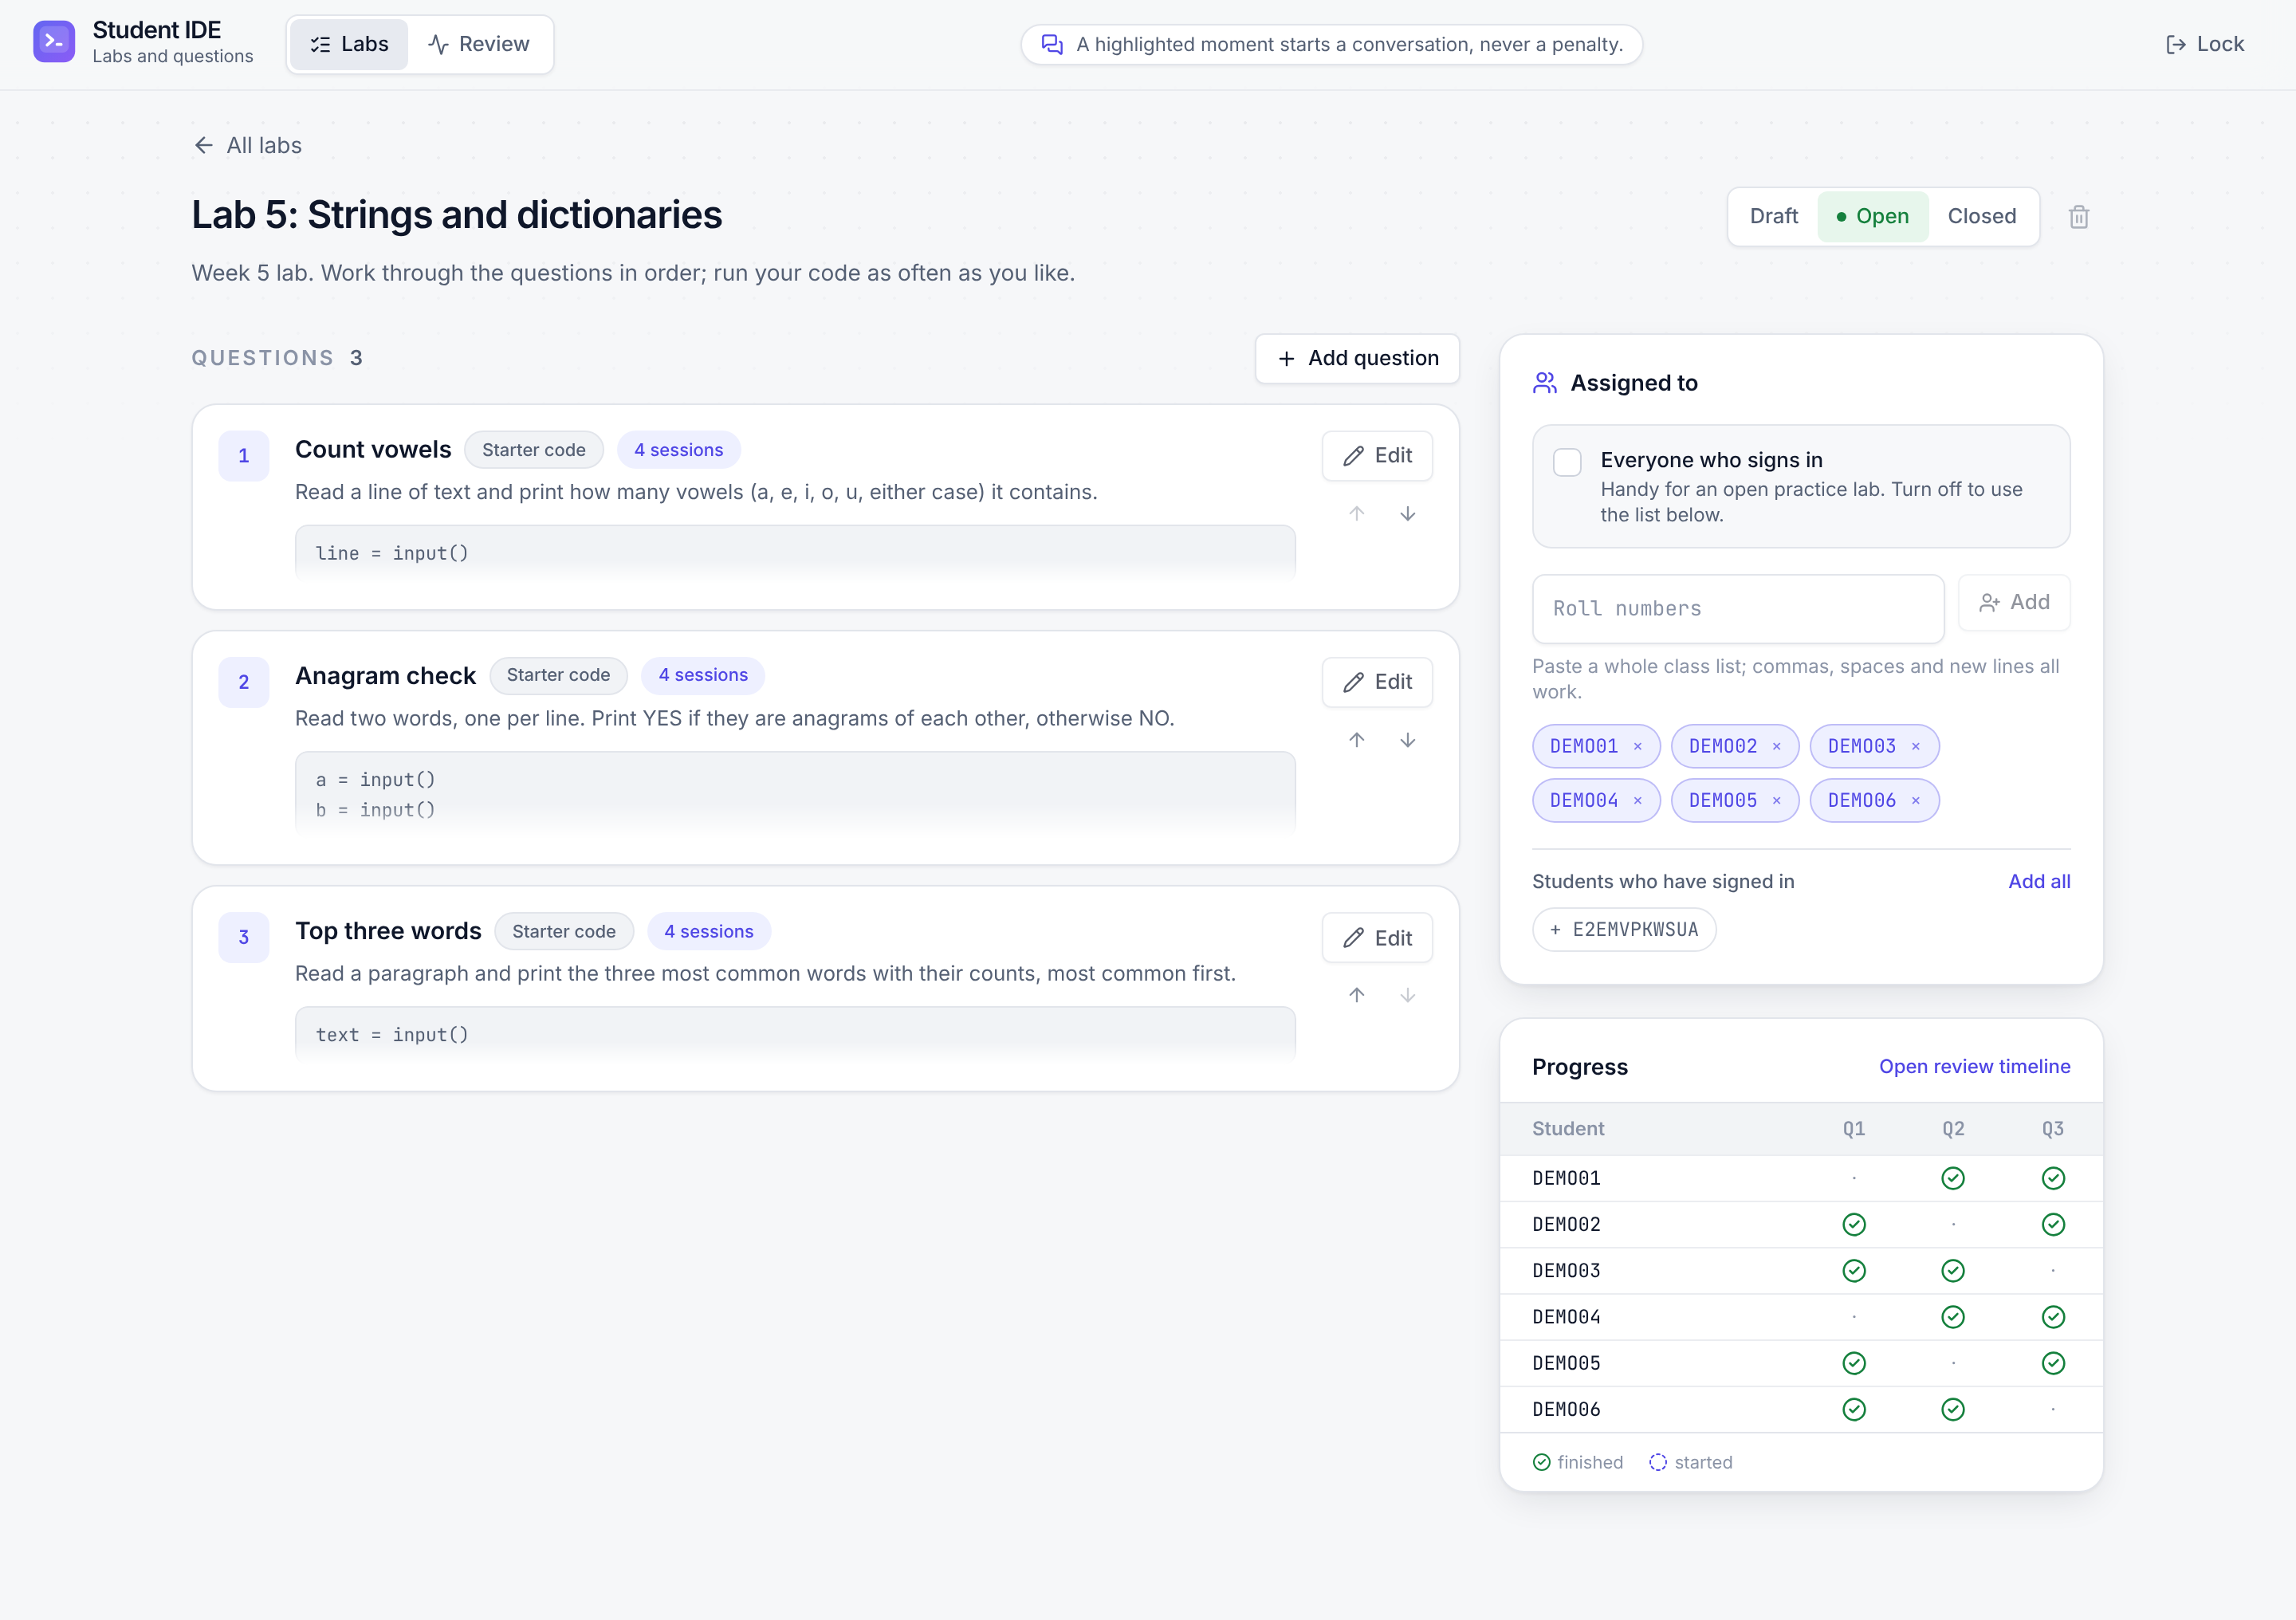
\includegraphics[width=\linewidth]{teach/teach-light-08-demo-lab}
    \caption{Teacher view of a lab: ordered questions with starter code, the
    roster, and who has started or finished each question.}
  \end{subfigure}\\[1ex]
  \begin{subfigure}{0.49\textwidth}
    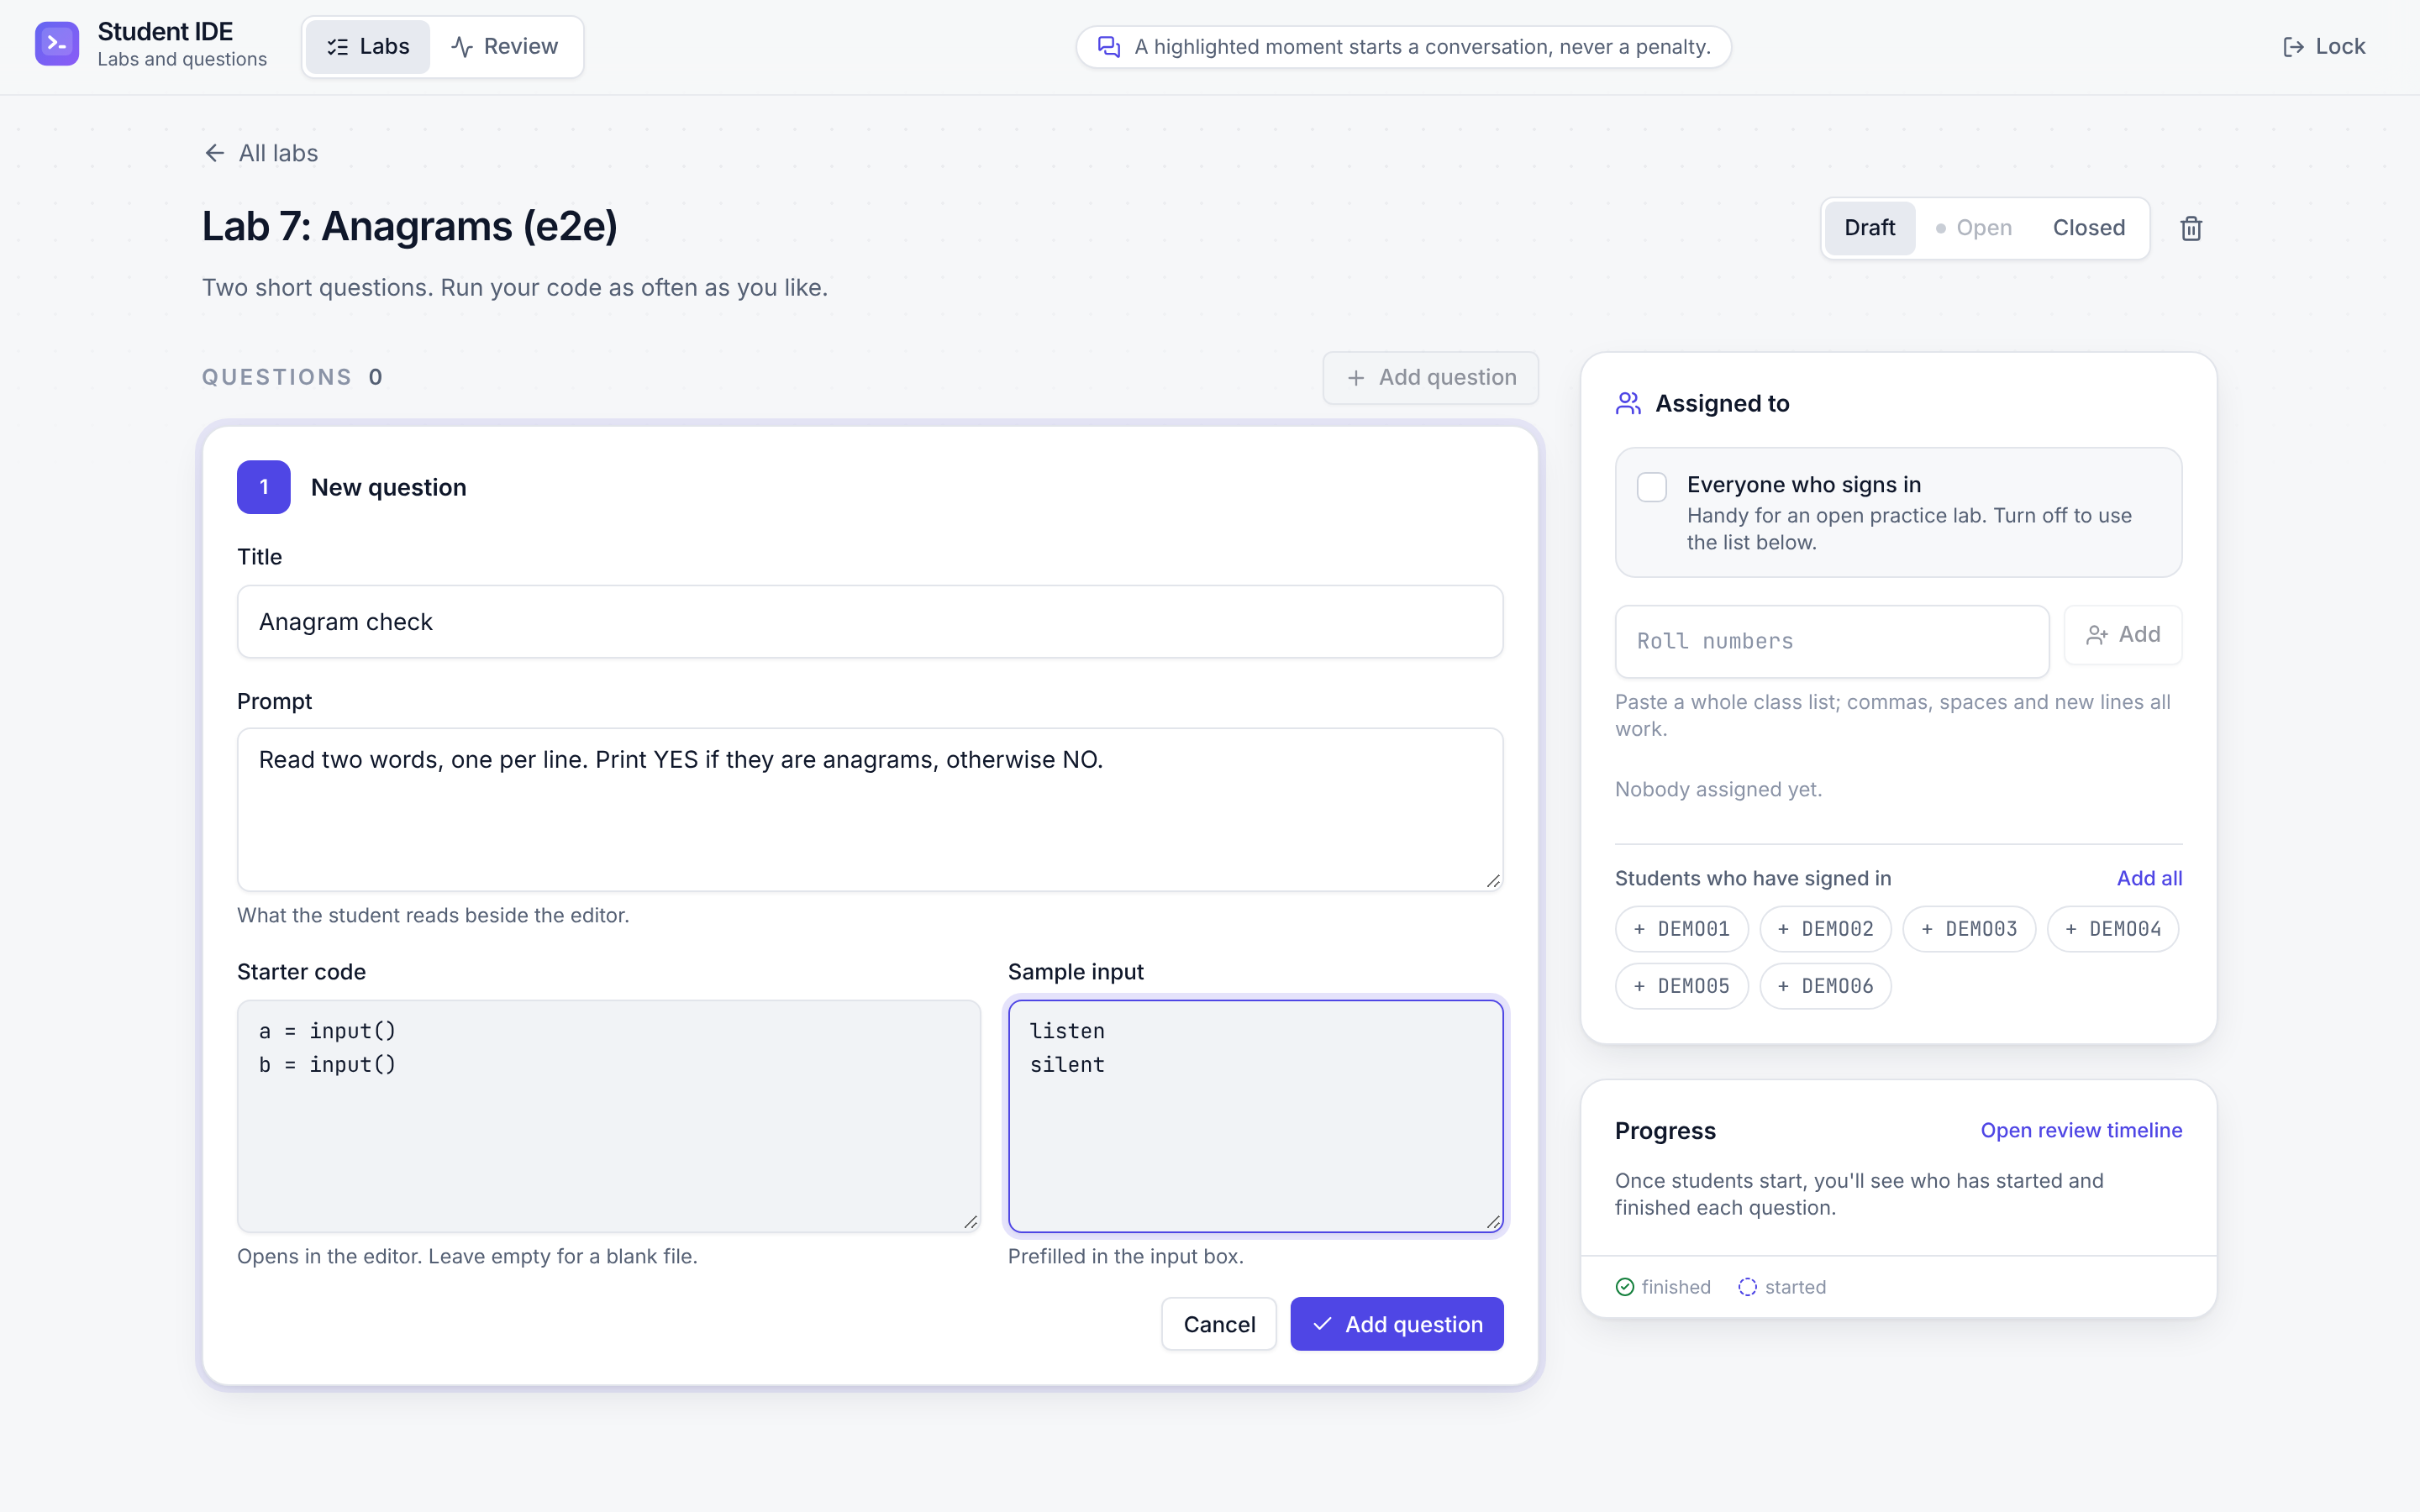
\includegraphics[width=\linewidth]{teach/teach-light-03-question-form}
    \caption{Adding a question.}
  \end{subfigure}\hfill
  \begin{subfigure}{0.49\textwidth}
    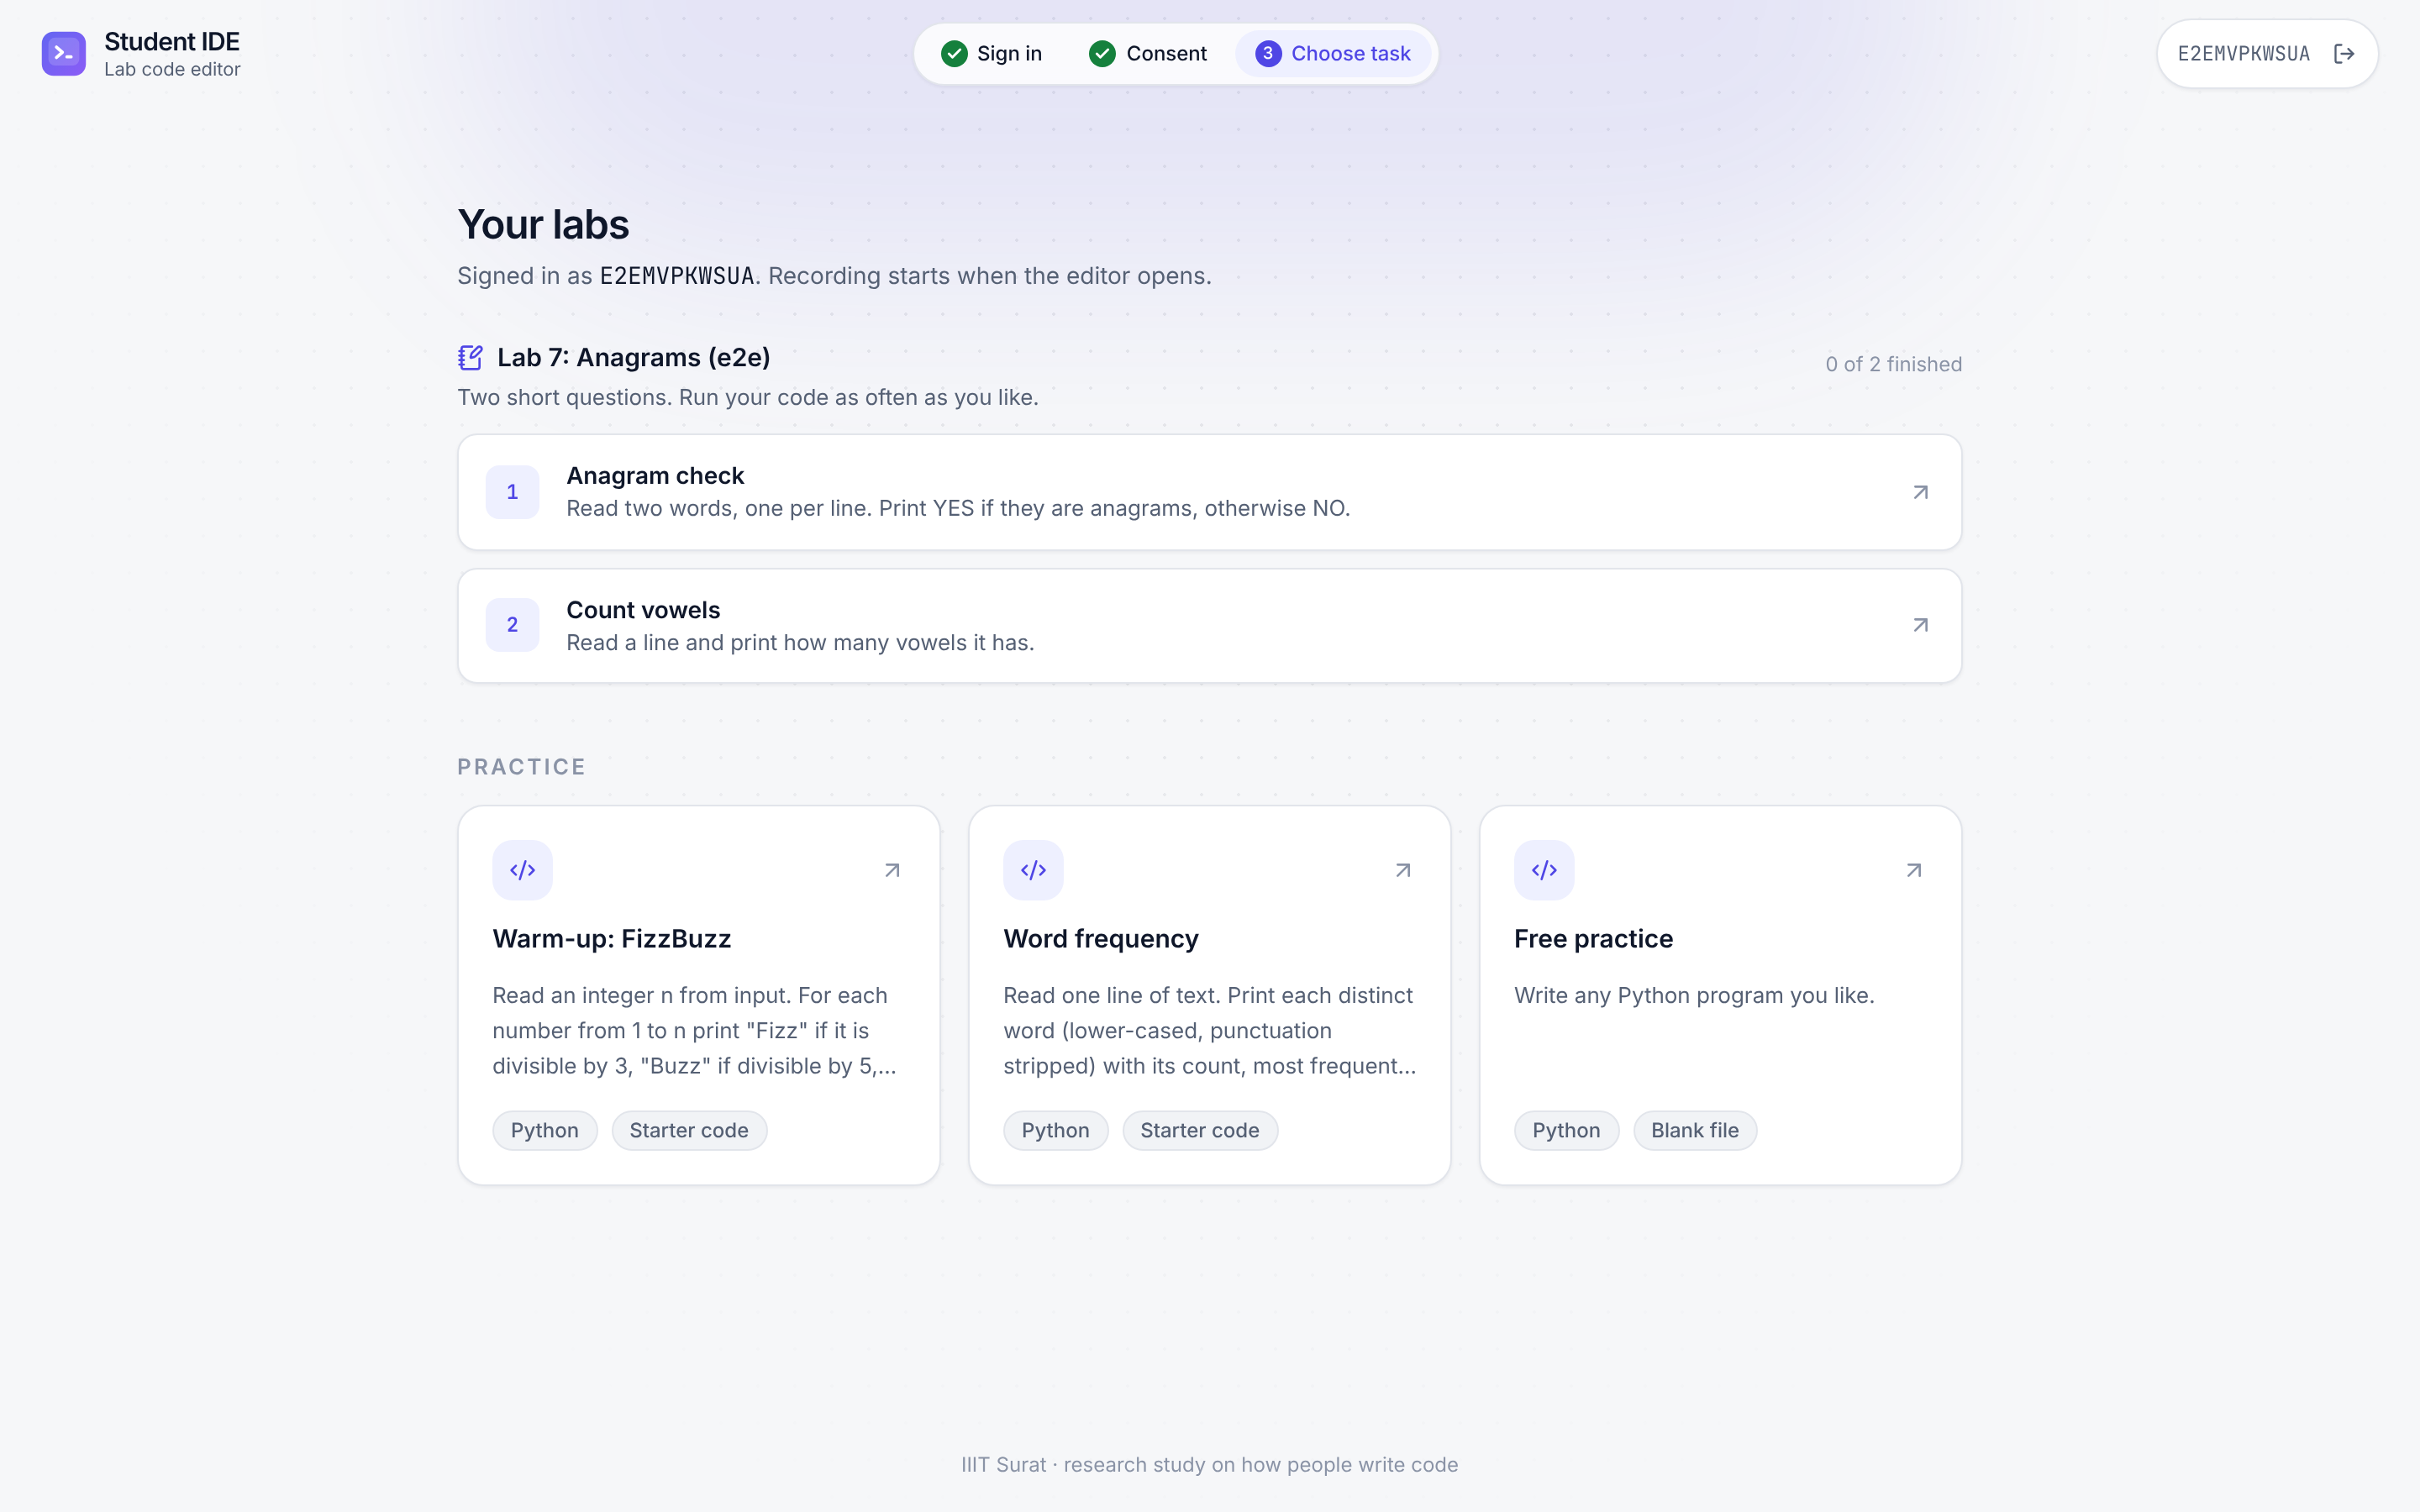
\includegraphics[width=\linewidth]{teach/teach-light-05-student-labs}
    \caption{What an assigned student sees after consent.}
  \end{subfigure}
  \caption{Labs and questions. Light and dark versions of every screen are
  in \texttt{snapshots/teach/}.}
  \label{fig:teach}
\end{figure}

\section{Class competitions}
\label{sec:competitions}
A competition is a lab run as a timed, class-wide challenge with a live
leaderboard (\cref{fig:compete}). It reuses the lab's questions, roster and
recorded sessions and adds a clock, a lobby in which students choose the name
shown on the board, and test-graded submissions. Ordinary labs treat
correctness as optional, since in class the effort is what matters; a
competition is the one place where correctness is scored. Every competition
question therefore needs at least one test case before the clock can start.
A submission earns $100 \times$ the share of tests passed, keeping the best
submission per question, plus up to 50 points for a full solve, scaled by the
share of the planned time still left. Wrong submissions cost nothing.

The board is kept deliberately gentle: by default students see the top ten
and their own place, never who is last; badges (first to solve, fastest per
question, solved them all, most bugs fixed) let more students stand out; and
only chosen board names are shown. The leaderboard reads nothing from the
detector or the review timeline, so a moment flagged for conversation can
never cost a place or become public. Competition sittings are recorded like
any lab; whether their time pressure changes typing enough to exclude them
from a student's baseline is left to the Phase~1 data.

\begin{figure}[ht]
  \centering
  \begin{subfigure}{0.49\textwidth}
    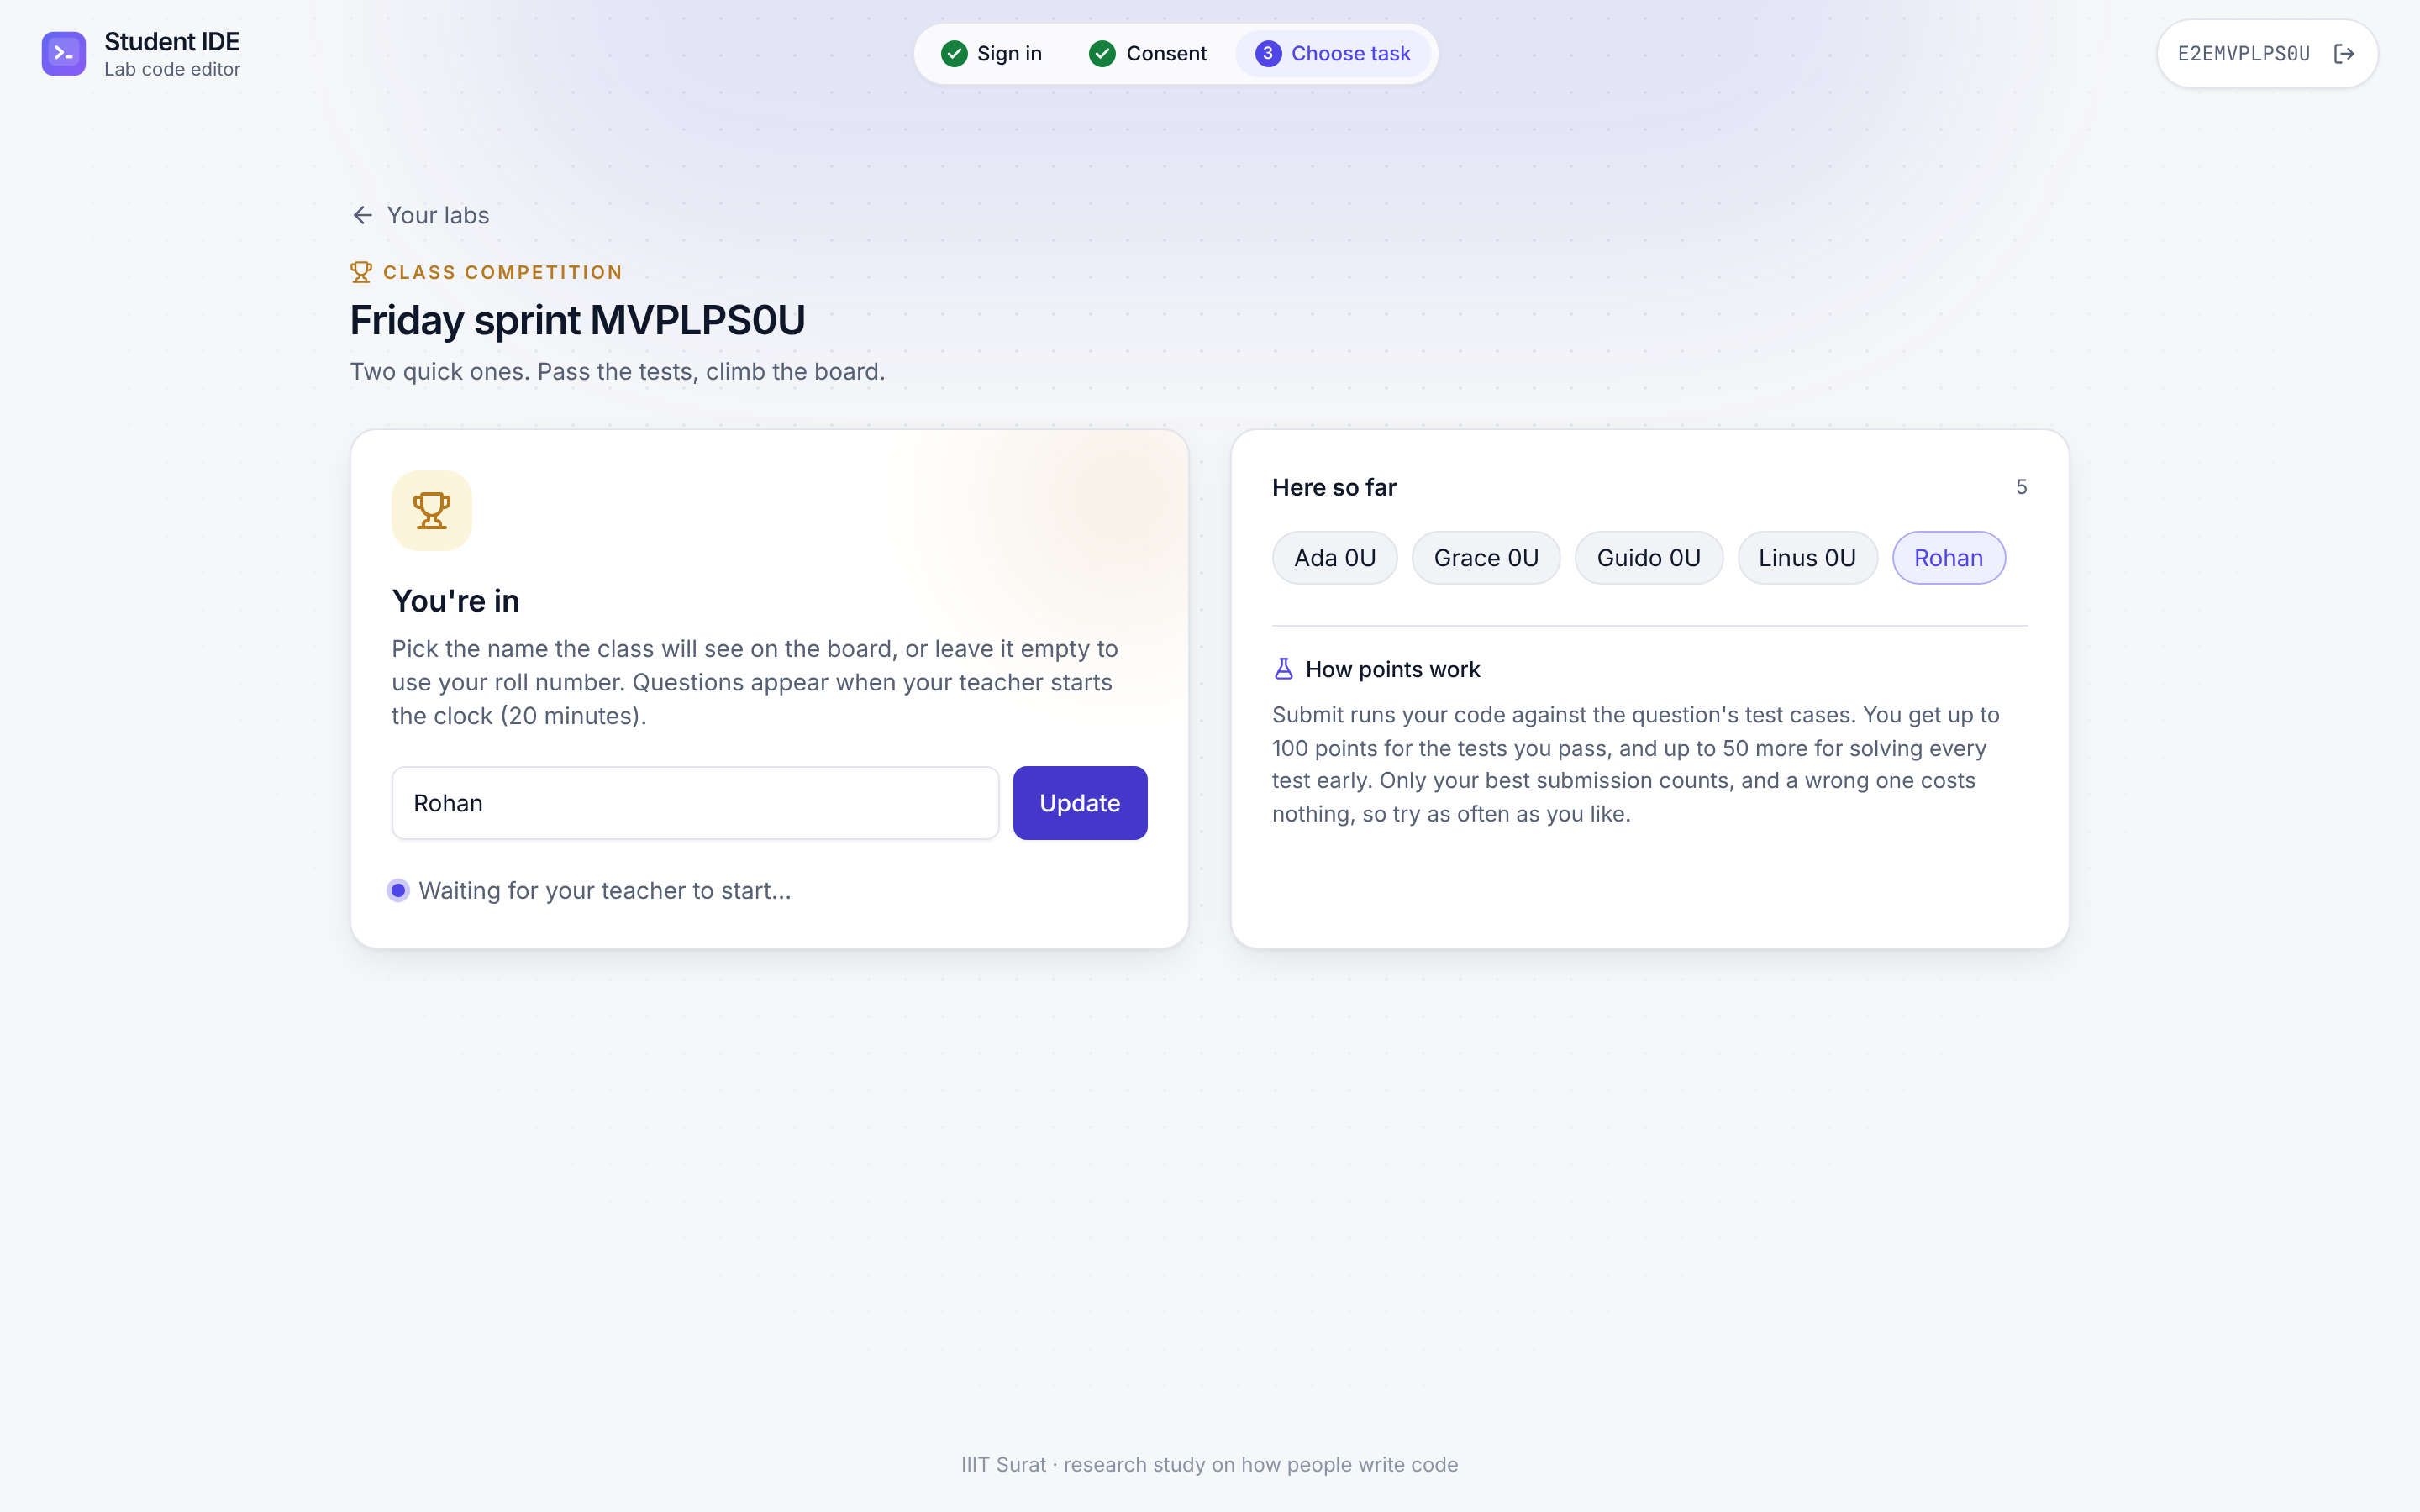
\includegraphics[width=\linewidth]{compete/compete-light-04-lobby}
    \caption{Lobby: students pick a board name before the clock starts.}
  \end{subfigure}\hfill
  \begin{subfigure}{0.49\textwidth}
    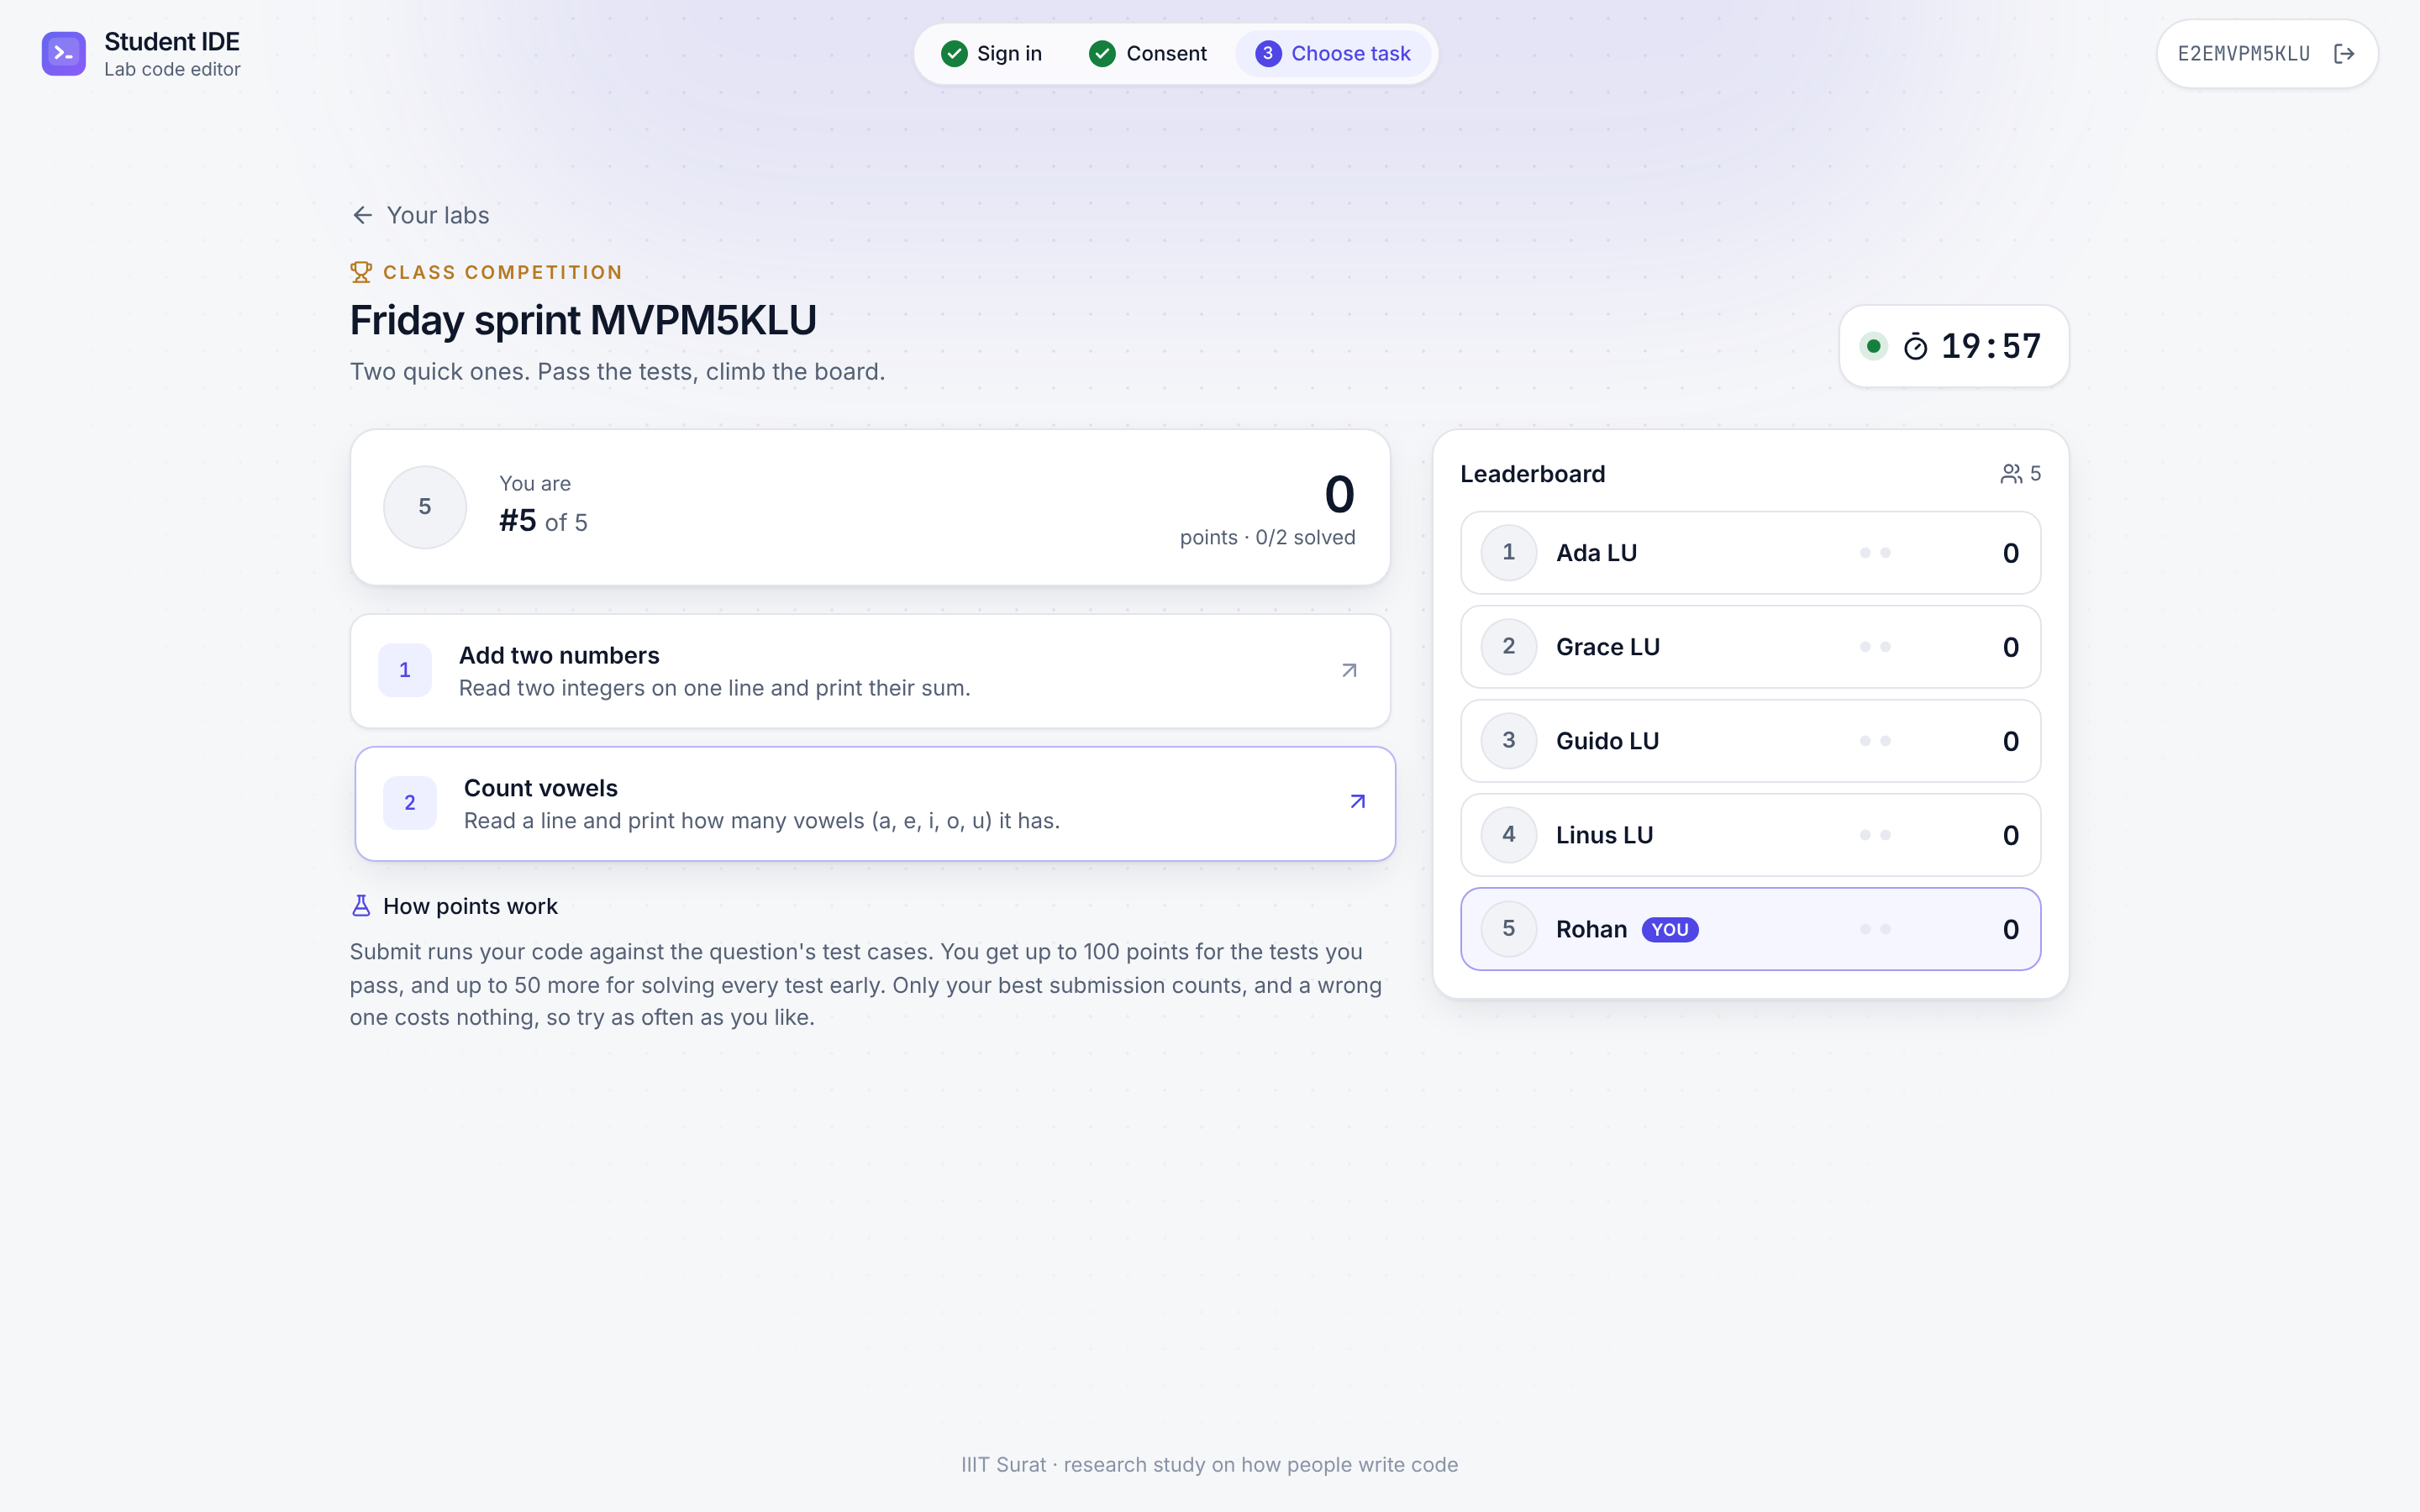
\includegraphics[width=\linewidth]{compete/compete-light-05-arena-live}
    \caption{Live: questions, own standing and the board.}
  \end{subfigure}\\[1ex]
  \begin{subfigure}{0.49\textwidth}
    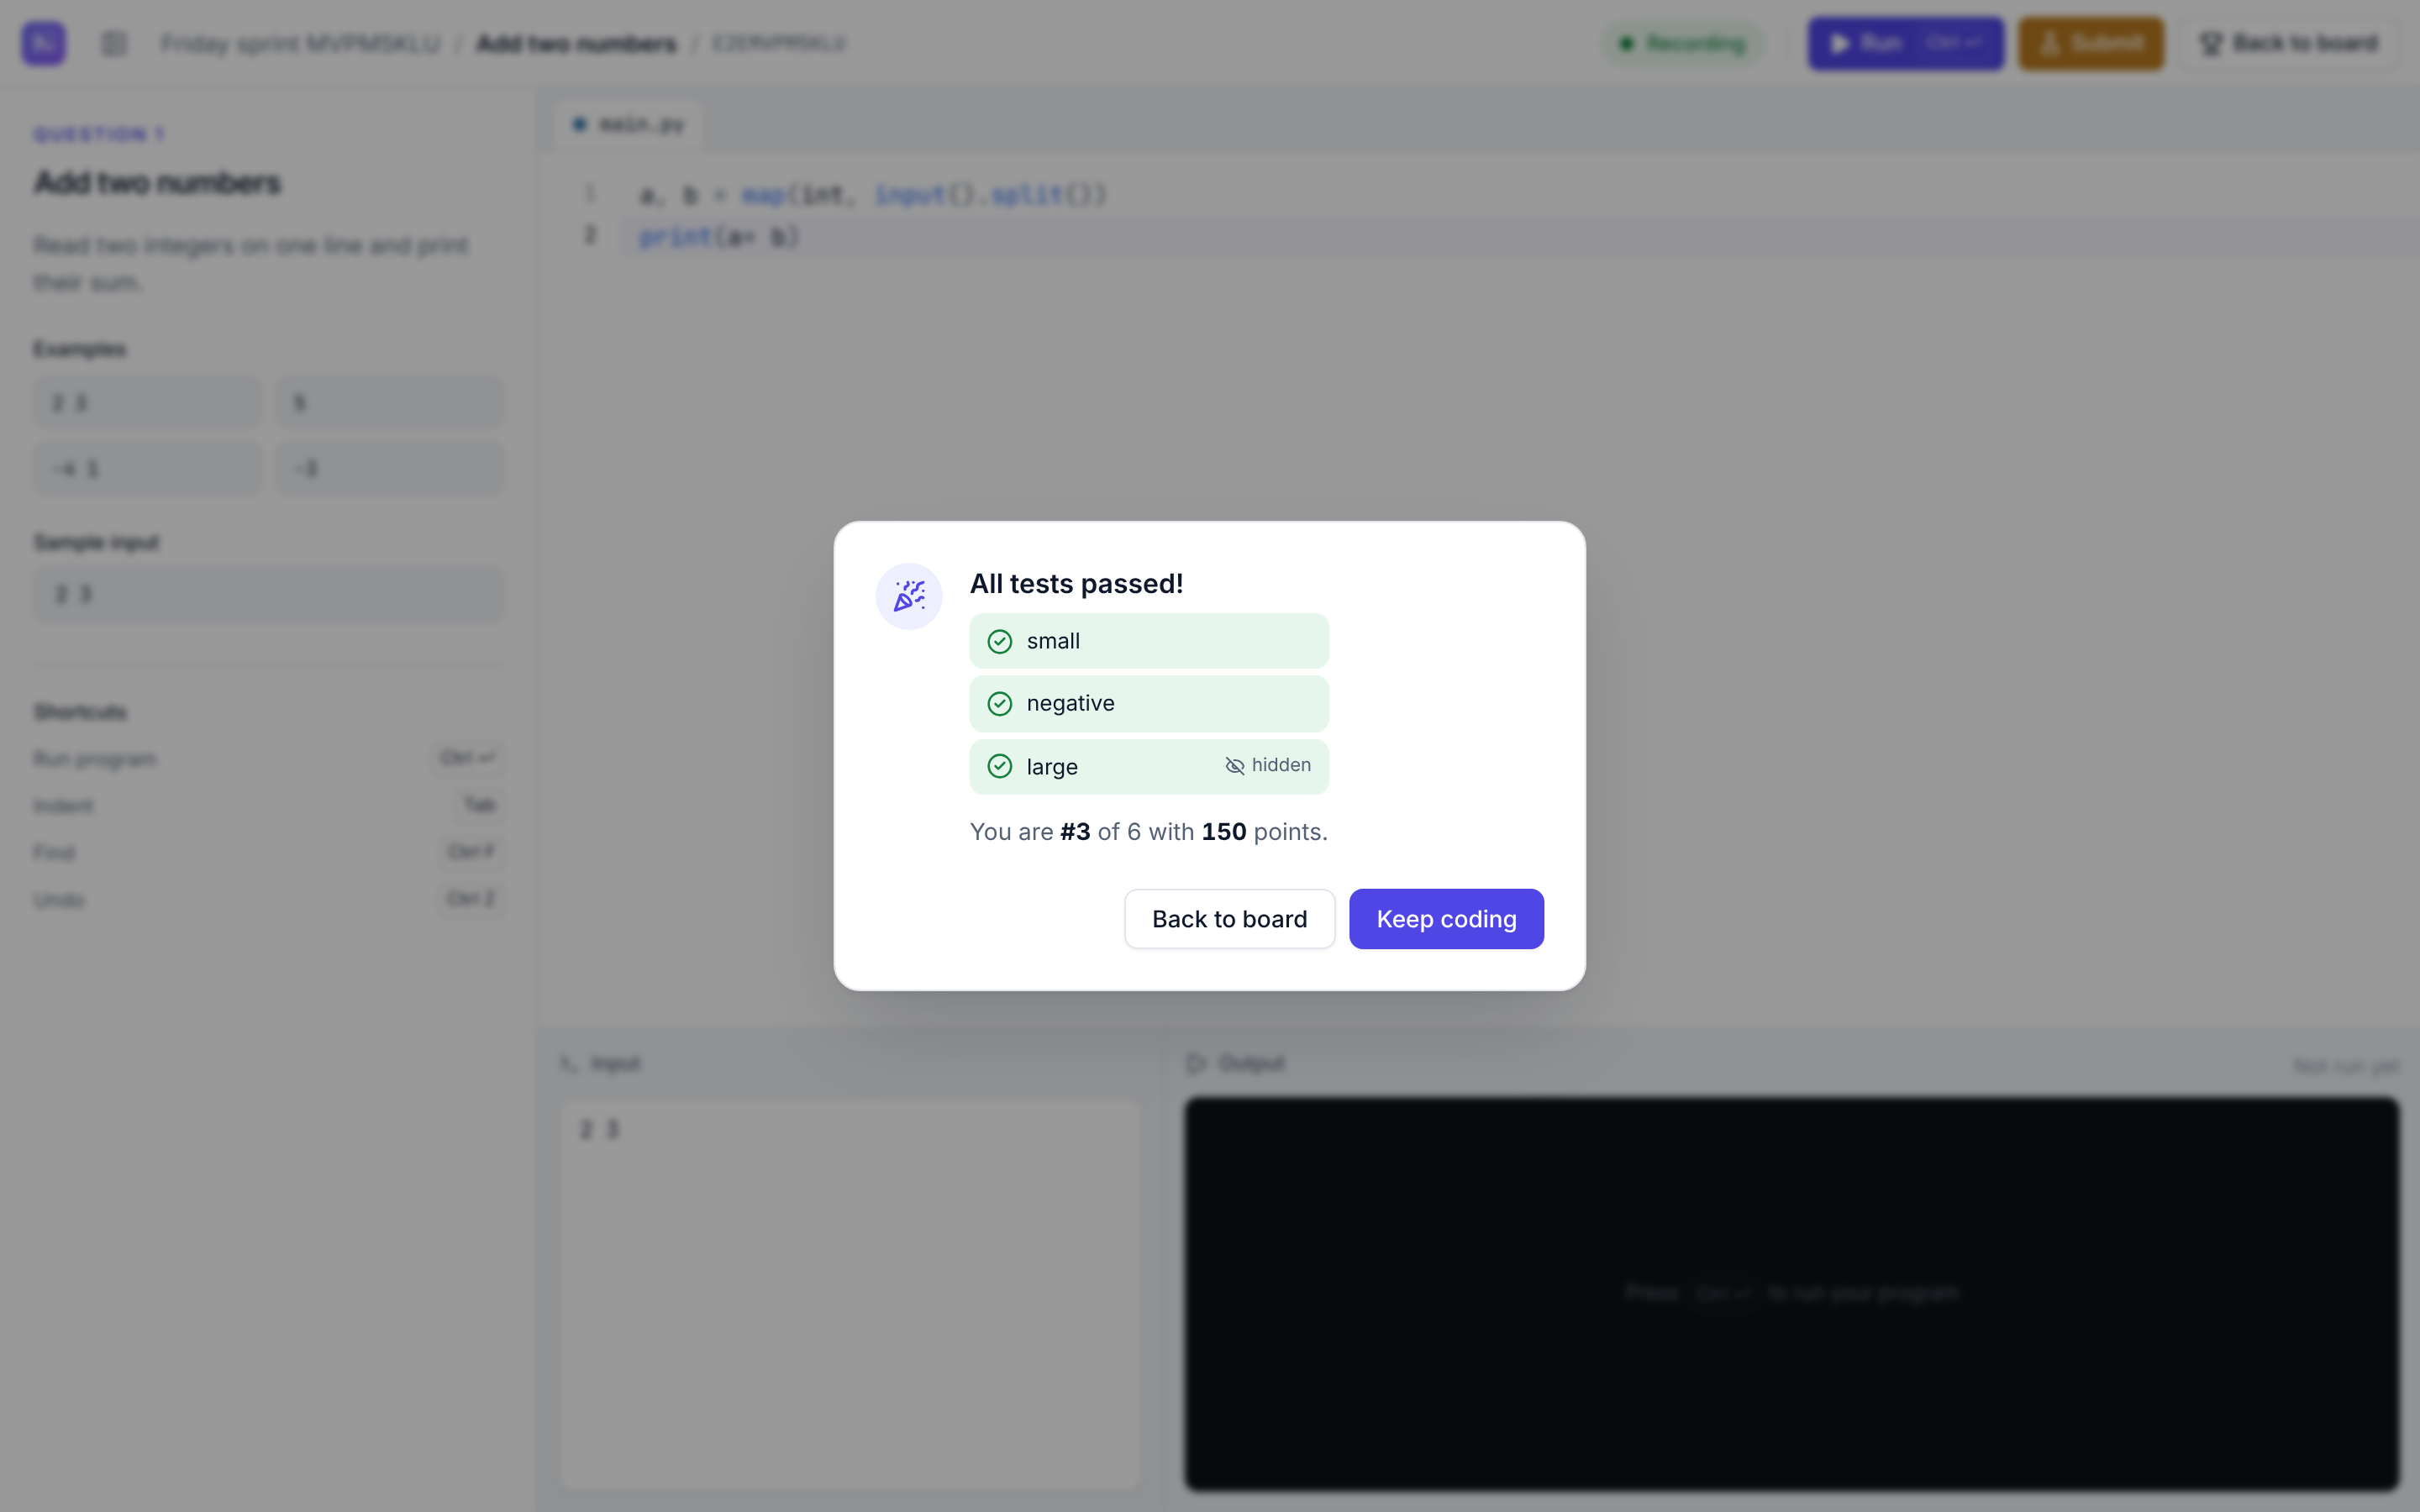
\includegraphics[width=\linewidth]{compete/compete-light-07-submit-solved}
    \caption{Submit runs the tests; hidden tests report pass or fail only.}
  \end{subfigure}\hfill
  \begin{subfigure}{0.49\textwidth}
    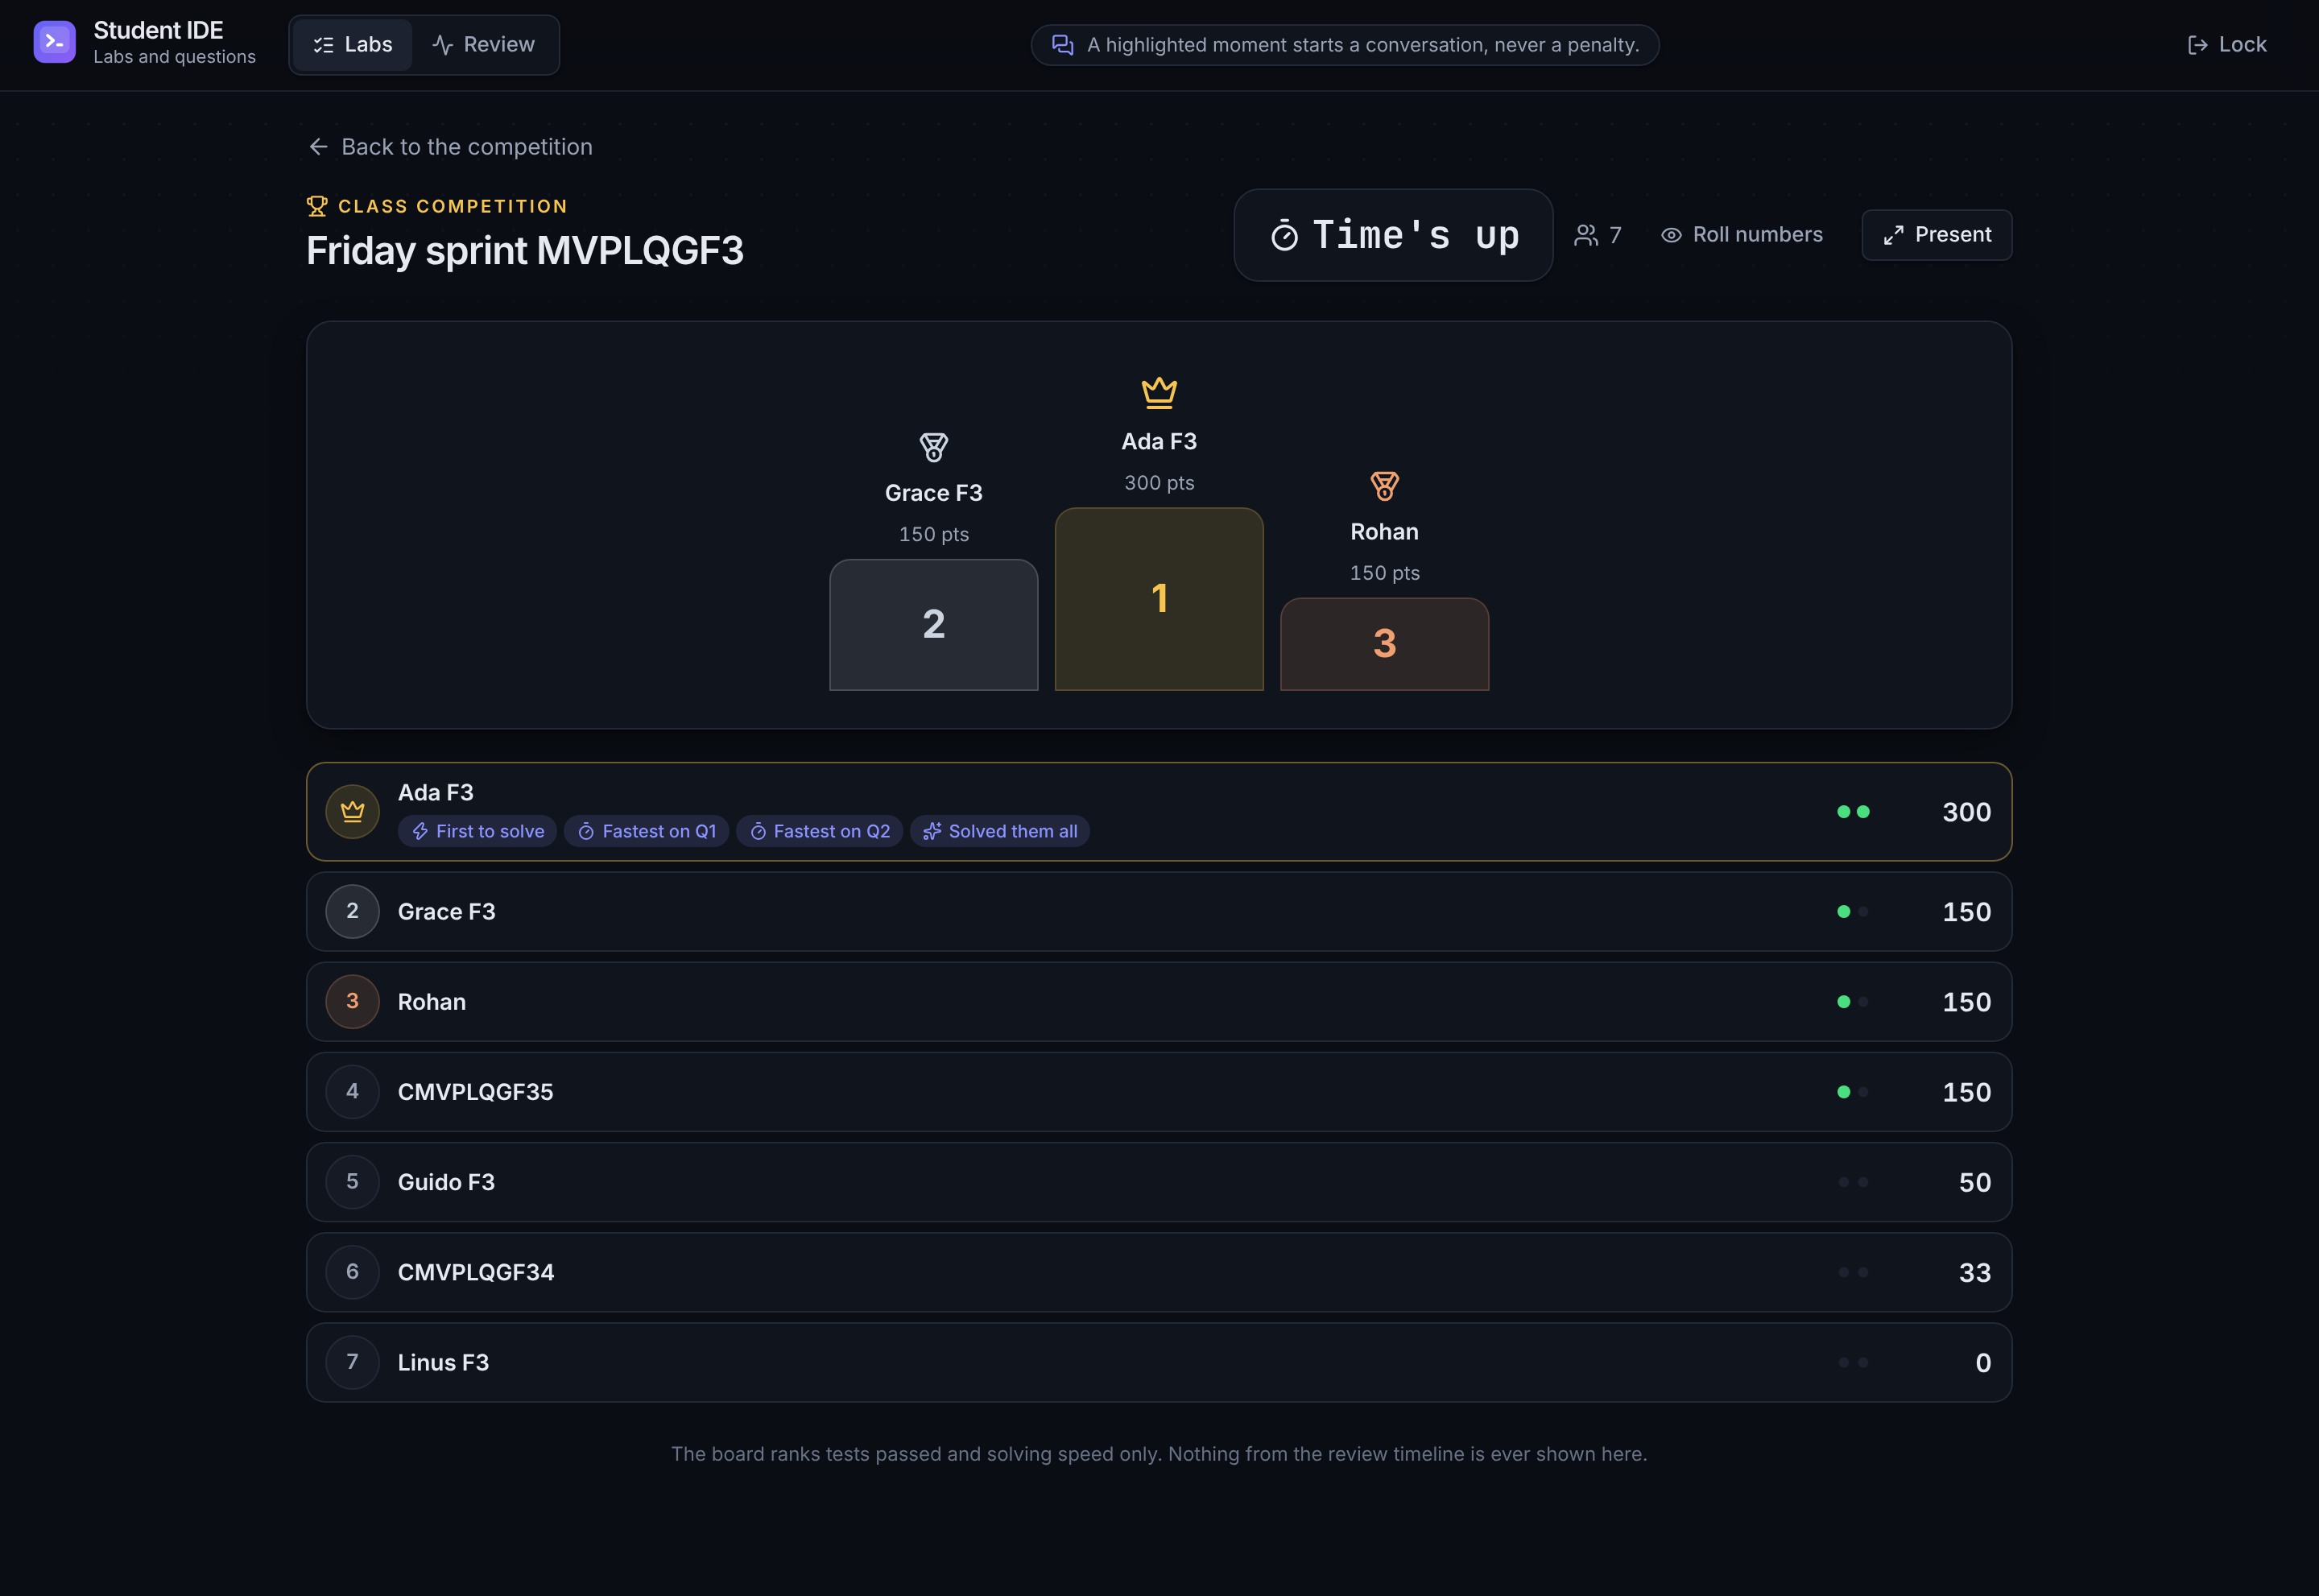
\includegraphics[width=\linewidth]{compete/compete-dark-09-podium}
    \caption{Teacher's projector board with the podium at the end.}
  \end{subfigure}
  \caption{Class competitions. All screens, light and dark, are in
  \texttt{snapshots/compete/}.}
  \label{fig:compete}
\end{figure}

\section{Teacher evidence timeline}
\label{sec:review-timeline}
The last part of the pipeline is a review screen for the teacher or
interviewer (\cref{fig:review-session}). It is opened from the same web
application under \texttt{\#/review}, but only with the research token
that also guards the raw-data API; without the token on the server the
whole review side is switched off. The token is kept in the browser tab
only.

\paragraph{What it shows.} An overview lists every session with a small
trace of both detector channels and the moments it found
(\cref{fig:review-overview}). Opening a session shows one time axis with,
from top to bottom: for each channel, a strip of per-window scores (how far
each \SI{30}{\second} window sits from the student's own baseline) and the
CUSUM trace drawn against its threshold; then pastes, times the student
left the editor, runs (clean or with an error) and typing activity. A
playhead can be dragged or played at 1--60$\times$; the code is rebuilt in
the browser from the recorded edits at that instant, with lines changed in
the previous \SI{30}{\second} tinted, and a strip of the last key-press
intervals shows the typing rhythm at that point. The replay was checked
against all 524 stored snapshots of eight sessions with no mismatch.

\paragraph{From alarms to moments.} CUSUM restarts after every alarm, so a
lasting change (for example, a second person typing for the rest of the
session) raises a chain of alarms, each starting where the previous one
fired. The screen merges such a chain into one \emph{moment to discuss},
with the detector's estimated start, the time it was first noticed and how
long the difference lasted. For each moment it lists the habits that moved
most between the estimated start and the first alarm, in the student's own
units (``time between keys: usual \SI{158}{\milli\second}, here
\SI{134}{\milli\second}'') with a bar for how many of the student's usual
spreads that is. These are the same per-feature $z$ values the detector
sums, so the explanation is the model rather than a story told about it.

\paragraph{Wording.} Nothing on the screen says ``flag'', ``cheating'' or
``suspicious''. A session either has \emph{moments worth a conversation}
or ``nothing stood out''. Every moment comes with three suggested
questions (walk me through this code; did anything change at that point;
make a small change while I watch) and the reminder that habits shift for
ordinary reasons and that no mark or penalty follows from the screen.
Baseline-week sessions are scored only against the student's other
baseline sessions and are labelled as a check of the baseline, not of the
student; students without enough baseline sessions are not scored at all.

\paragraph{The screen runs the evaluated detector.} The review screen reads
the configuration the evaluation harness froze
(\texttt{thesis/evaluation/frozen-config.json}, \cref{sec:rq1-harness}), so
what a teacher sees is what was evaluated: three lanes (typing rhythm and
key-pair timing on \SI{30}{\second} windows, way of working on
\SI{90}{\second} windows), each with its own CUSUM $k$, the population prior
for short baselines and the thresholds $h$ calibrated on the dev students.
Each lane is drawn on its own window grid against one time axis. The
population parts (feature weights, the key-pair vocabulary, the prior) are
fitted on the class's own baseline sessions once three students have one,
just as the harness fits them on its training students. Thresholds can be
overridden once they are calibrated on the class's real data.

\paragraph{Demo data.} \texttt{python -m studentide.seed} fills a fresh
database with simulated students (four honest baseline weeks, then
sessions under the study conditions). Their ground truth is stored with
the session and can be overlaid on the timeline
(\cref{fig:review-session}b), which made the screen testable before any
real student was recorded. It is refused on an existing database file so
demo and real data never mix. On the default demo (six simulated students,
twelve assessed sessions) with the frozen configuration, seven of the eight
non-honest sessions got a moment on the expected kind of lane (one
speed-matched takeover was missed), none of the four honest sessions did,
and none of the 24 baseline-week sessions did either (with the earlier
untuned thresholds and no prior, 5 of 24 baseline-week sessions had raised
a moment). This is a check that the screen shows the detector faithfully,
not an evaluation (that is \cref{ch:rq1}).

\begin{figure}[ht]
  \centering
  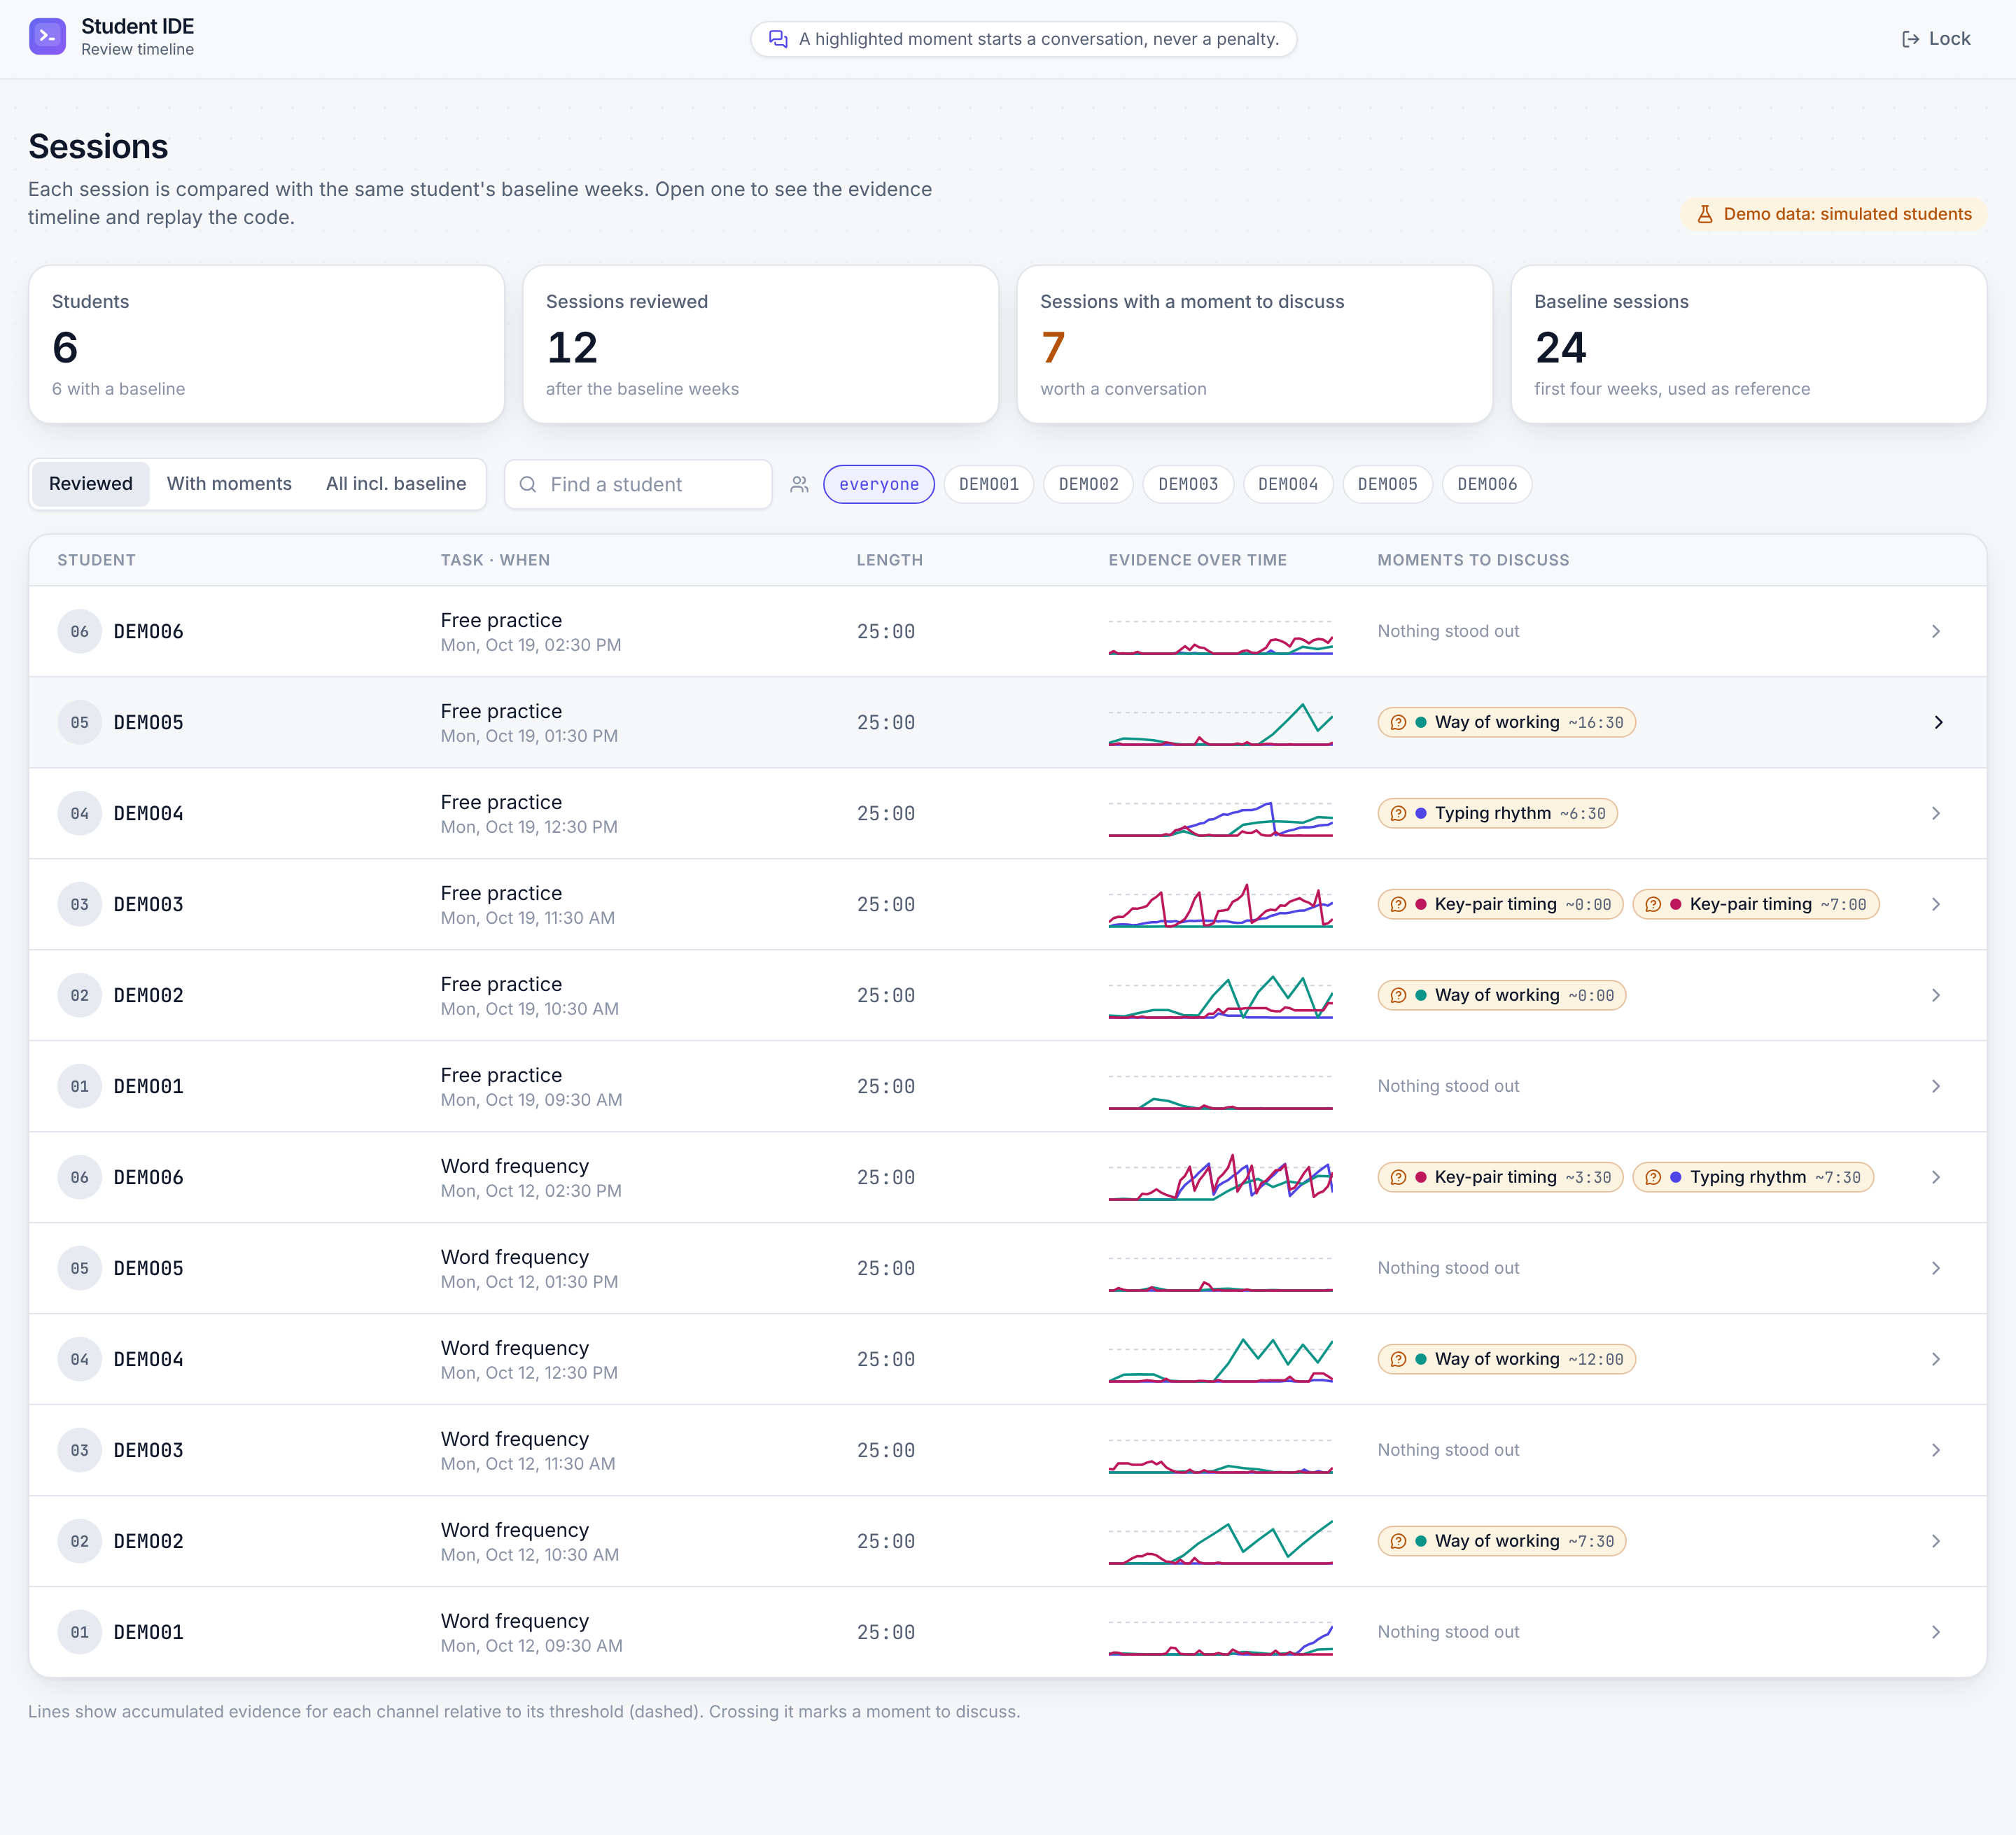
\includegraphics[width=\linewidth]{review/review-light-02-overview}
  \caption{Review overview on simulated students: each row shows every
  channel's accumulated evidence relative to the threshold (dashed) and
  the moments to discuss, with the channel that found them.}
  \label{fig:review-overview}
\end{figure}

\begin{figure}[ht]
  \centering
  \begin{subfigure}{\textwidth}
    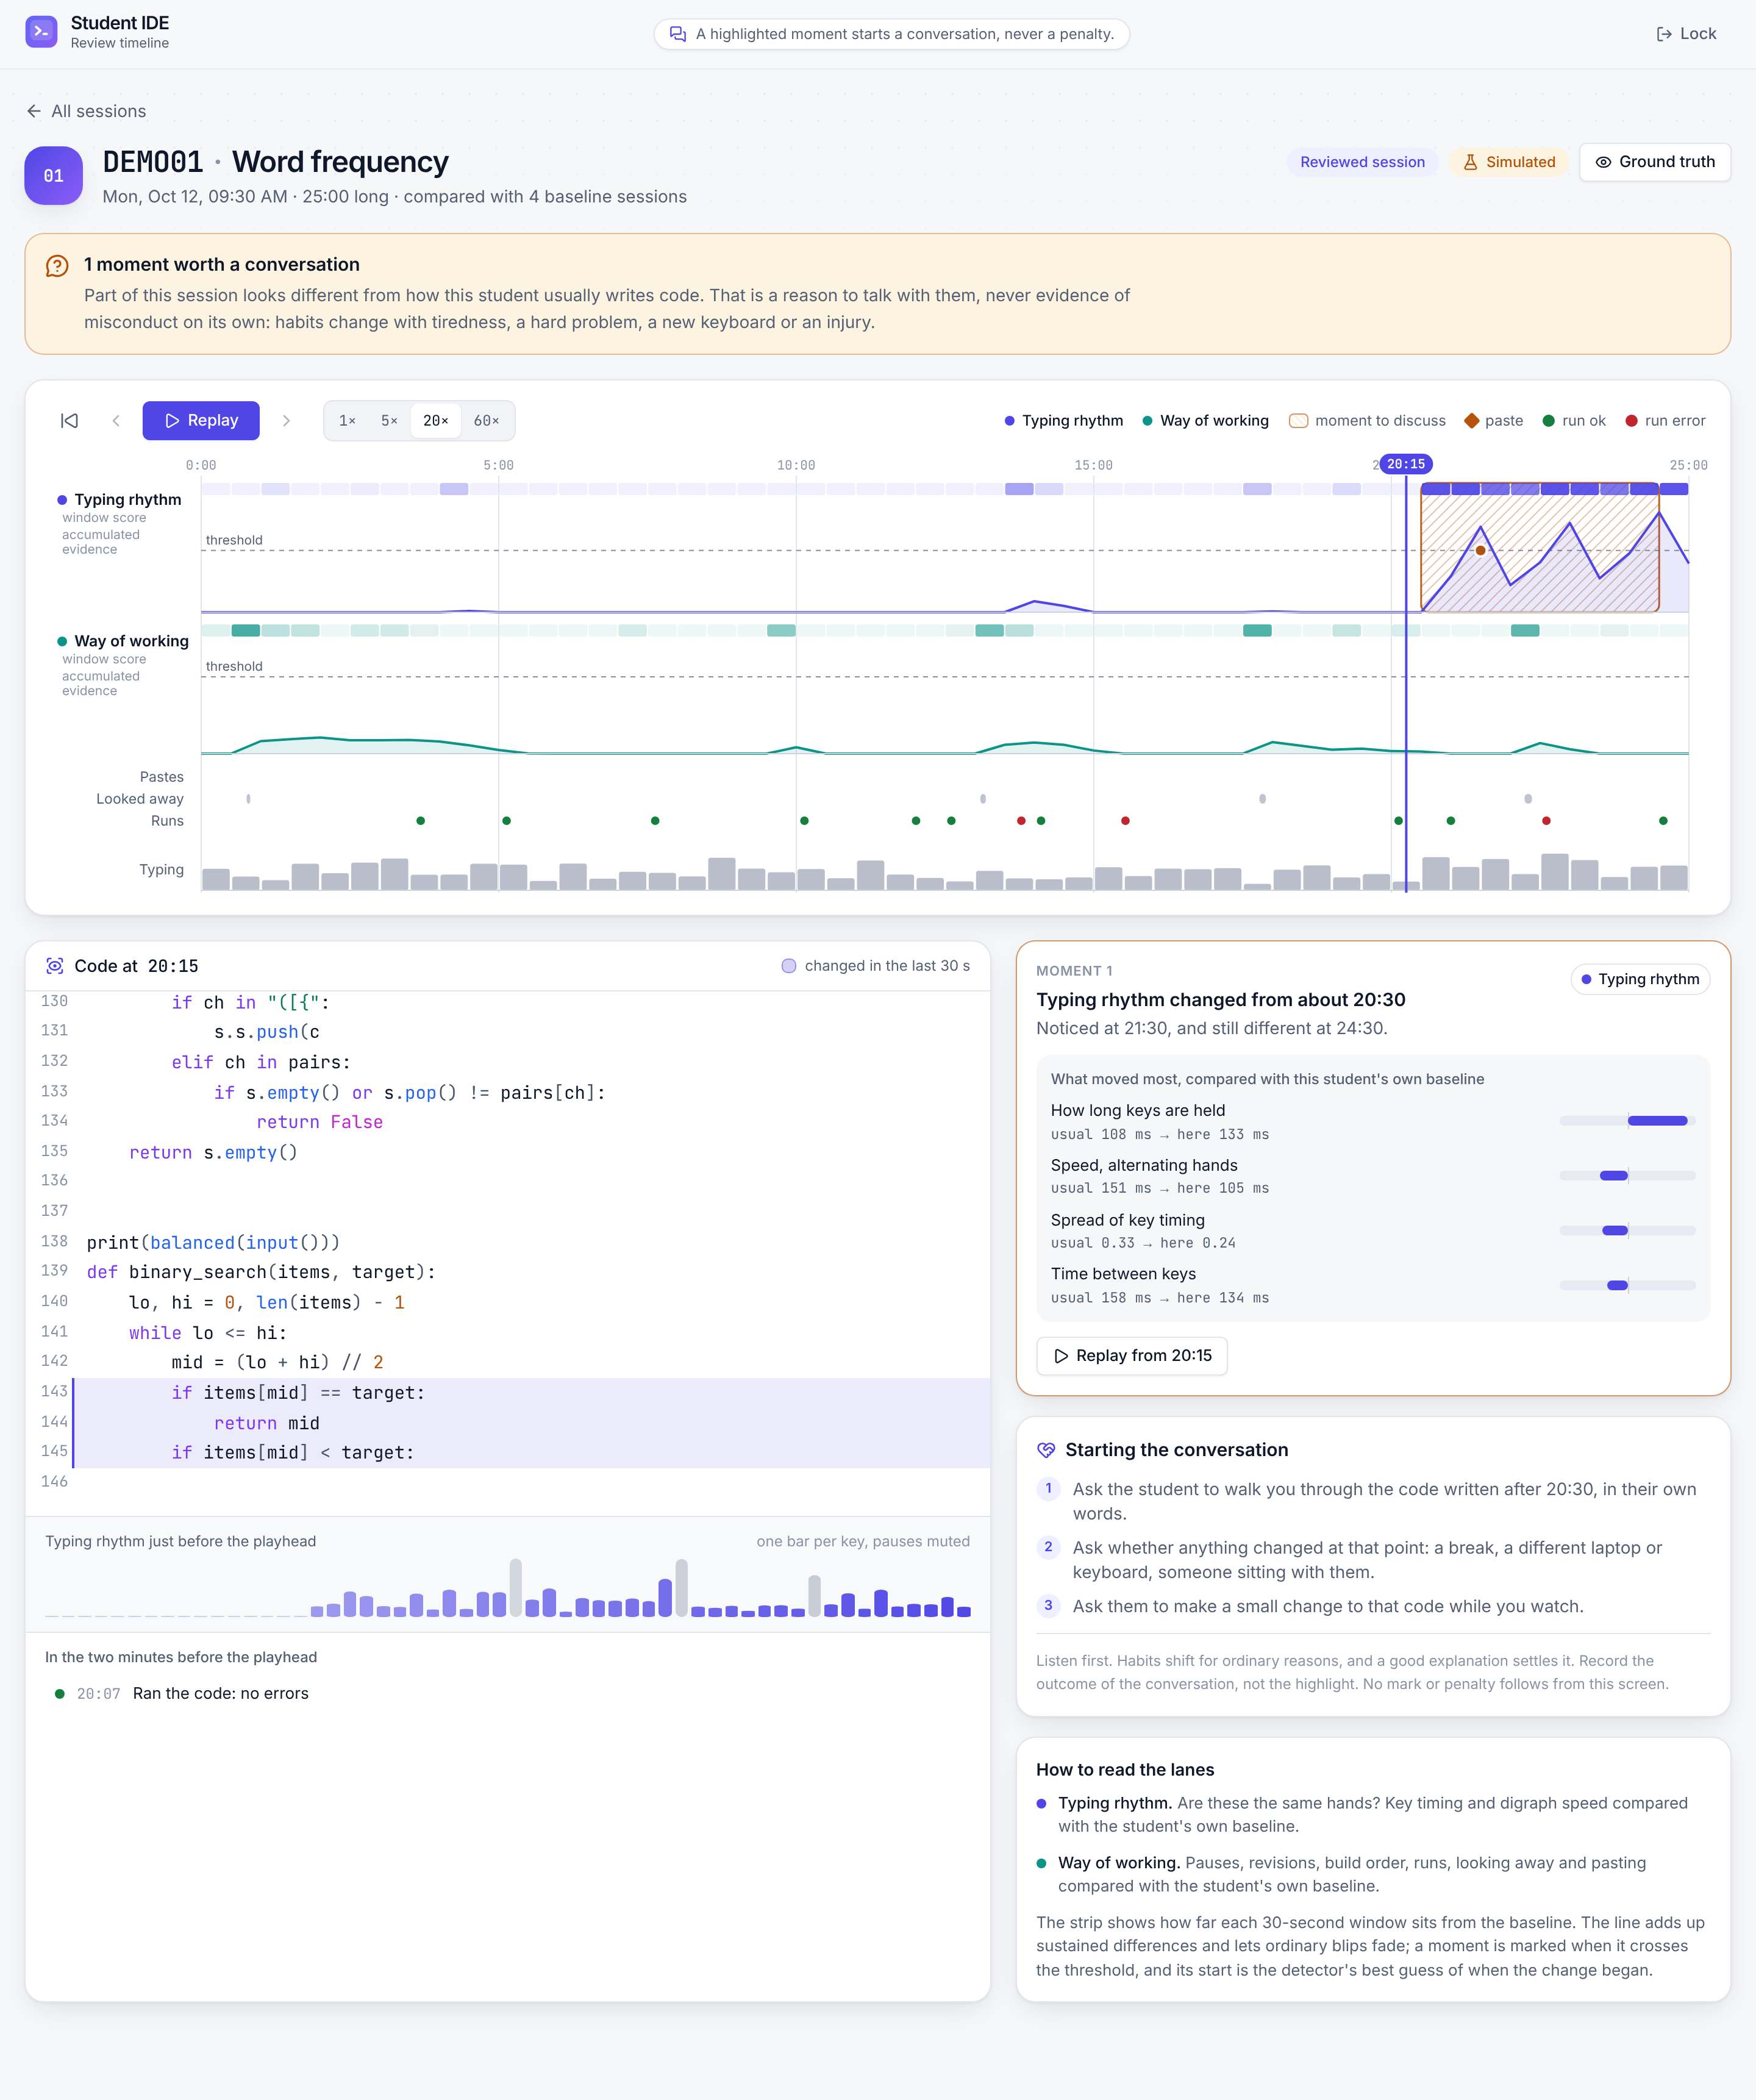
\includegraphics[width=\linewidth]{review/review-light-03-session-takeover}
    \caption{A simulated takeover: the typing-rhythm and key-pair lanes mark
    moments; the replay shows the code at the playhead.}
  \end{subfigure}\\[1ex]
  \begin{subfigure}{\textwidth}
    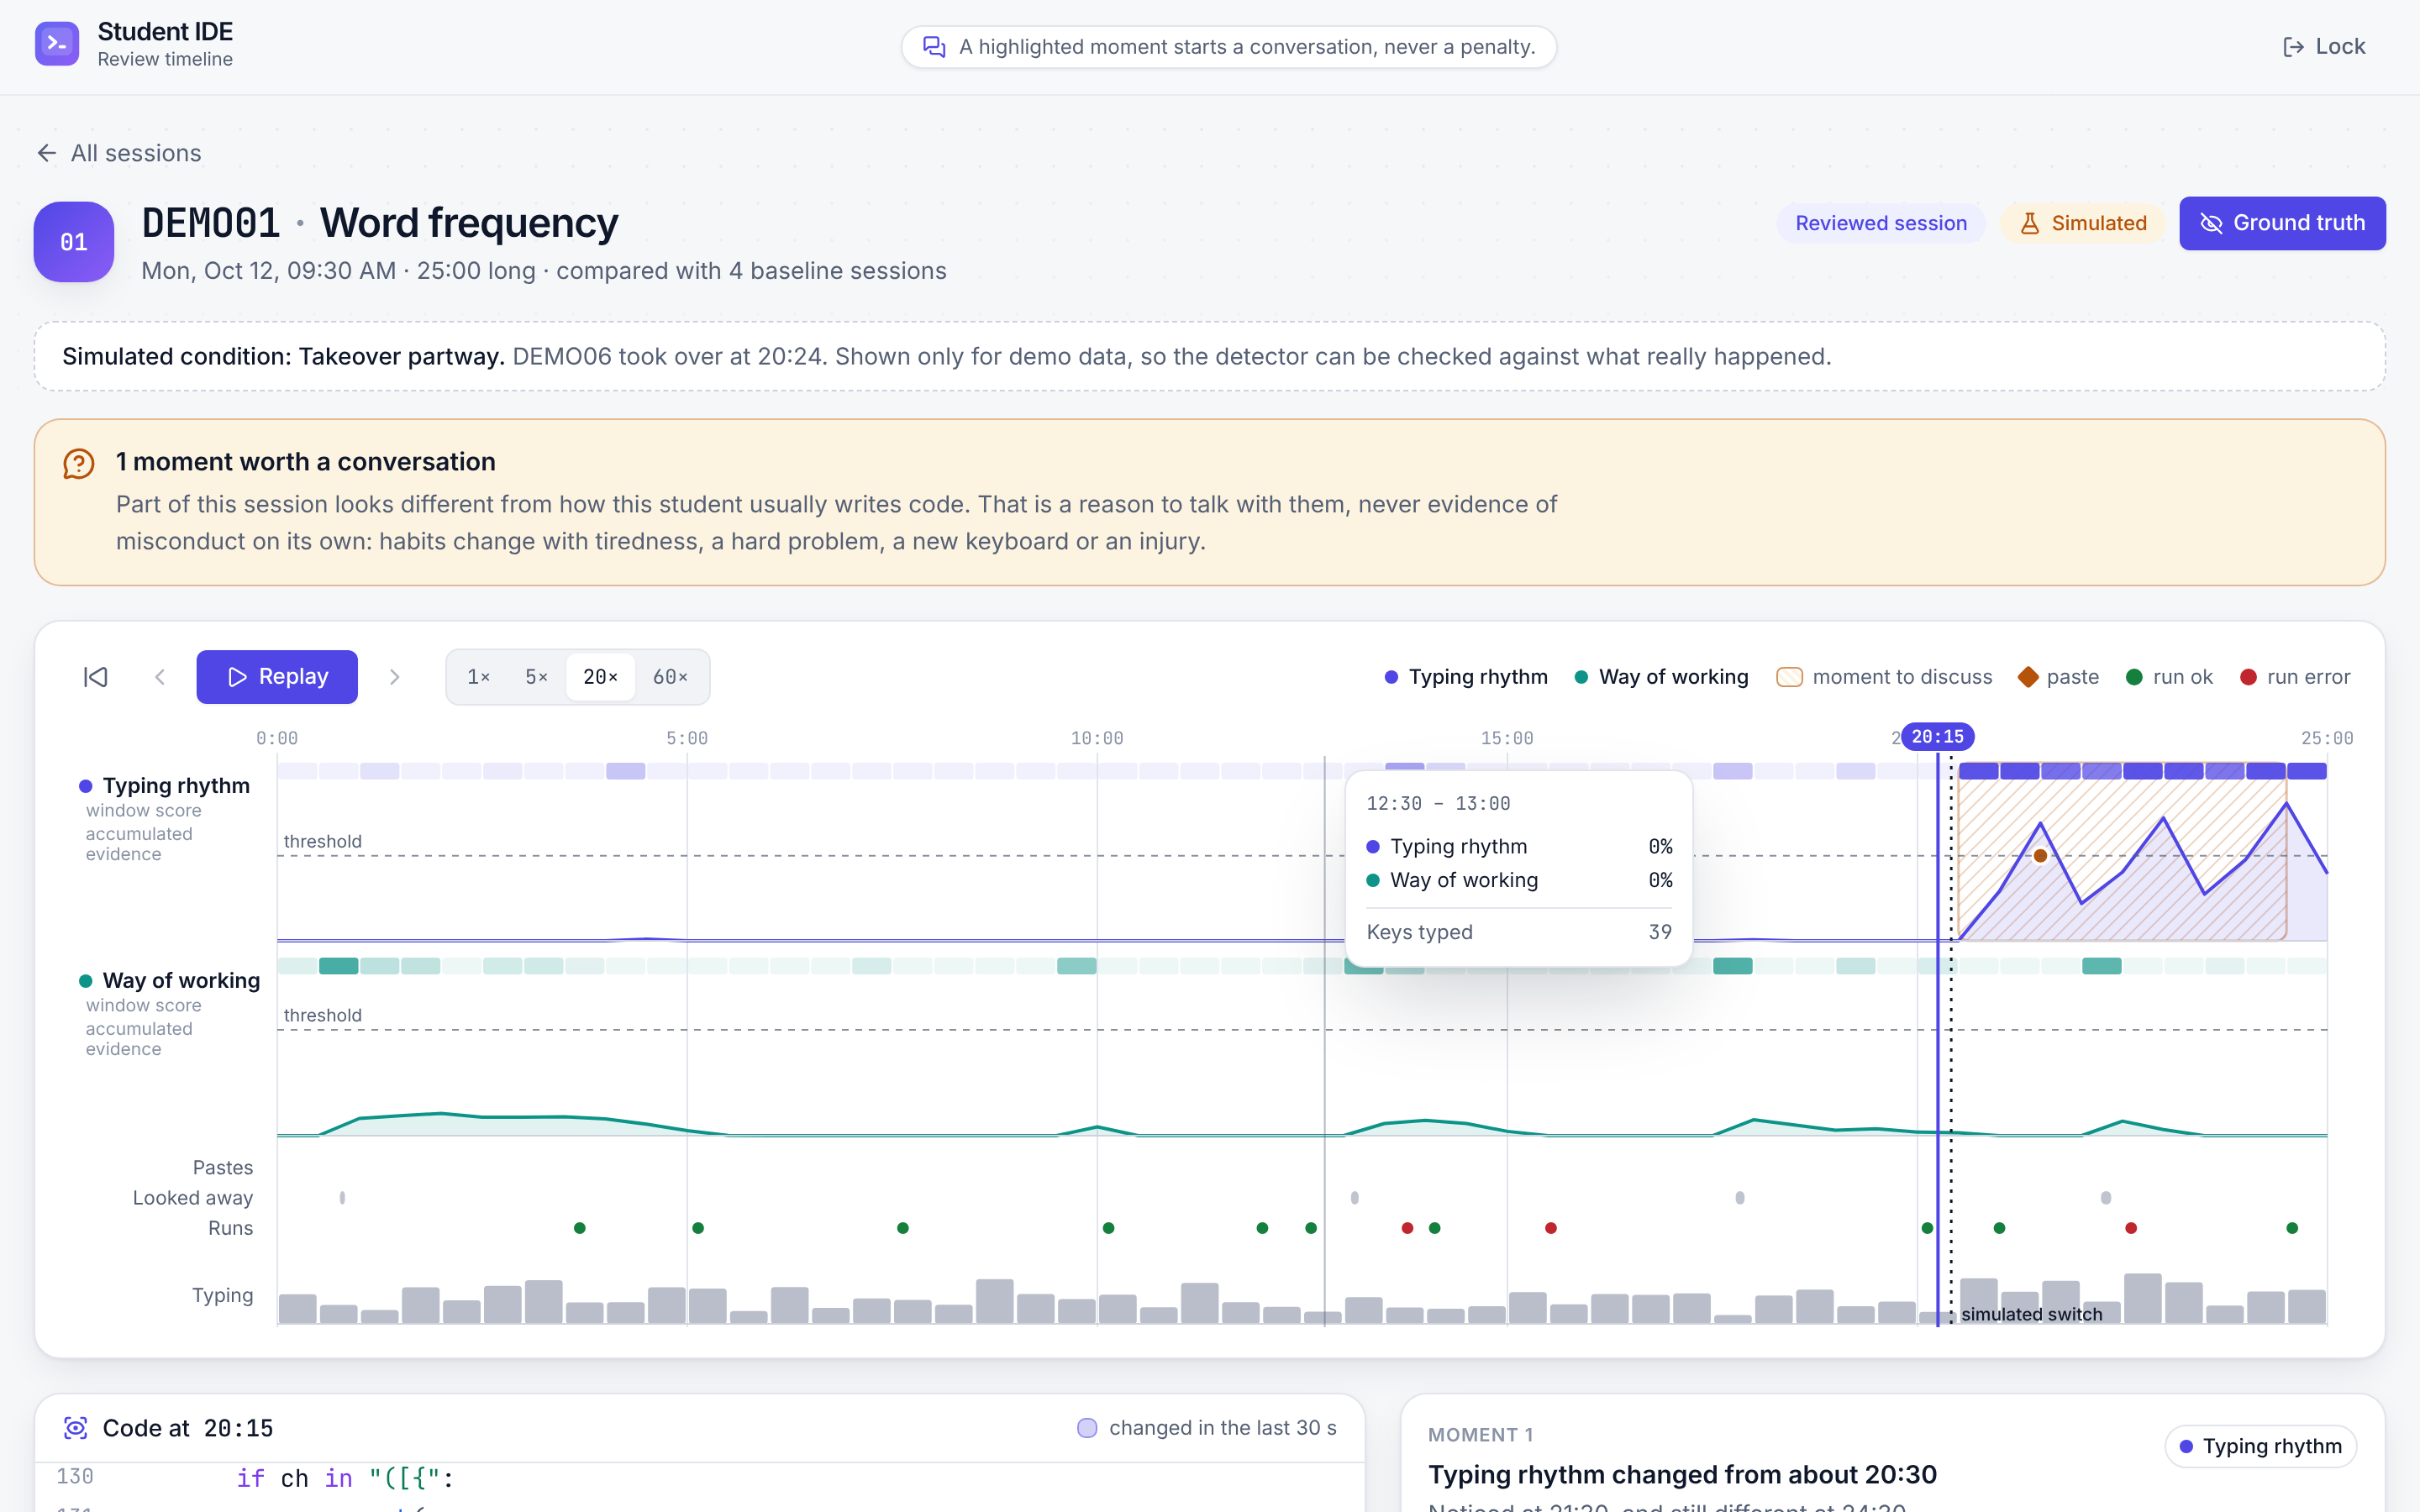
\includegraphics[width=\linewidth]{review/review-light-04-takeover-truth-hover}
    \caption{Same session with the simulated ground truth (switch at 7:43)
    overlaid and the hover read-out for one window. The key-pair lane's
    first moment is dated well before the switch, a reminder that the
    estimated start is a guess.}
  \end{subfigure}
  \caption{Session review timeline. Light and dark versions of every
  screen are in \texttt{snapshots/review/}.}
  \label{fig:review-session}
\end{figure}

\chapter{Habit Features and the Switch Detector}
\label{ch:detector}

% Draft written with the phase 2 code (backend/studentide/detector/).
% Brain entries 2026-10-26-09 to -12.

\Cref{fig:detector} summarises the detector. The event log of a session is
cut into windows of $W$ seconds; each window becomes a vector of habit
features; two channels compare that vector with the student's own baseline
and feed a CUSUM change-point detector each. An alarm on either channel
marks the session for review, with an estimate of when the change happened
and which kind of change it was.

\begin{figure}[ht]
  \centering
  \resizebox{\linewidth}{!}{\tikzfig{detector}}
  \caption{The two-channel switch detector.}
  \label{fig:detector}
\end{figure}

\section{Windowing}
Windows are consecutive and non-overlapping, $W=30$\,s by default (the
window length is ablated in \cref{tab:ablation-window-length}). A window
counts only if it holds at least 20 code keystrokes; inactive windows
(reading, thinking, away) leave the detector state unchanged rather than
pulling it towards ``normal''. Keys pressed with Ctrl or Meta held,
modifiers and navigation keys are not part of the typing stream.

Keystrokes typed while the caret is inside a \texttt{\#} comment are kept
apart from code keystrokes. Lueder et al.\ observed that comment text is
typed like retyping, fluently and with few pauses \cite{lueder2026nosi}, so
mixing it in would blur the code rhythm. The comment status of each key is
recovered by replaying the edit stream (\cref{app:schema}) and checking
whether a \texttt{\#} outside a string precedes the caret on its line.
Comment keys get two features of their own, which the detector does not
use by default.

\section{Habit features}
\Cref{tab:features} lists the features. Latencies are on a log scale, so a
difference means the same for slow and fast typists. A digraph is two
consecutive code keystrokes with no deletion between them and a gap below
2\,s; longer gaps are pauses. The L-scale (second L-moment
\cite{hosking1990lmoments}) of log inter-key time is the spread measure Nosi
uses to separate composing from transcribing \cite{lueder2026nosi}.

\begin{table}[ht]
  \centering\small
  \caption{Habit features per window and the channel that uses them.}
  \label{tab:features}
  \begin{tabularx}{\linewidth}{@{}llX@{}}
    \toprule
    Group & Feature & Definition \\
    \midrule
    rhythm & \texttt{dg\_median} & median digraph latency (log ms) \\
     & \texttt{dg\_lscale} & L-scale of log inter-key time \\
     & \texttt{hold\_median} & median key hold time (log ms) \\
    digraph & \texttt{dg\_alt\_hand}, \texttt{dg\_same\_hand} & median latency when hands alternate / repeat \\
     & \texttt{dg\_to\_space}, \texttt{dg\_from\_space} & median latency into / out of the space bar \\
     & \texttt{dg\_shifted} & median latency into a shifted character \\
    \midrule
    pauses & \texttt{pause\_per\_100}, \texttt{pause\_median} & pauses ($\ge 2$\,s) per 100 keys; their median length \\
    revision & \texttt{del\_per\_100}, \texttt{del\_burst} & deletions per 100 keys; mean run of deletions \\
    build order & \texttt{nonappend\_frac}, \texttt{jump\_rate} & share of edits not at the end of the file; caret jumps $>2$ lines per minute \\
    runs & \texttt{run\_rate} & runs per minute over the trailing 5 minutes \\
    focus & \texttt{focus\_out\_rate} & window/tab focus losses per minute \\
    paste & \texttt{paste\_frac} & share of inserted characters that were pasted \\
    \midrule
    comments & \texttt{c\_dg\_median}, \texttt{c\_key\_frac} & comment digraph latency; share of keys in comments (not scored) \\
    \bottomrule
  \end{tabularx}
\end{table}

\section{Per-student baseline}
A student's baseline is fitted on their honest sessions from the first four
lab weeks and keeps only summary statistics: for every feature a robust
centre (median) and spread ($1.4826\times$ MAD, with a small floor so that a
habit the student never varies, such as pasting, does not explode), plus the
mean $\mu_0$ and standard deviation $\sigma_0$ of the student's own distance
score. $\mu_0$ and $\sigma_0$ are estimated leave-one-session-out, so they
describe a \emph{new} honest session rather than the sessions the centre was
fitted on. Nothing else is stored, which lets the raw baseline keystrokes be
deleted as promised on the consent screen.

\section{Distance score and the two channels}
For window $t$ and feature $f$, $z_{tf}=|x_{tf}-c_f|/s_f$, clipped at 6.
The distance is a weighted root mean square,
\begin{equation}
  d_t=\sqrt{\frac{\sum_f w_f z_{tf}^2}{\sum_f w_f}},\qquad
  x_t=\frac{d_t-\mu_0}{\sigma_0}.
\end{equation}

A single score over all features turned out to be a poor compromise
(\cref{tab:ablation-feature-groups}): equal weights let the many noisy
process features drown the typing rhythm, and weighting by how well a
feature separates students drowns the process features that reveal copying
and pasting. The detector therefore runs two channels:
\begin{description}
  \item[Identity] (rhythm and digraph groups) asks whether the same hands
  are typing. Weights $w_f$ are the intraclass correlation of the feature
  across students' baseline windows \cite{shrout1979icc}, between-student
  variance over total variance. They need only honest baseline data from all
  students, no impostor examples.
  \item[Process] (pauses, revisions, build order, runs, focus, paste), equal
  weights, asks whether the way of working changed. It catches copying out
  and pasting by the student themselves, which the identity channel cannot
  see.
\end{description}

\section{CUSUM change-point detection}
Each channel runs a one-sided CUSUM \cite{page1954continuous,basseville1993detection}
on its standardised score,
\begin{equation}
  S_t=\max(0,\,S_{t-1}+x_t-k),
\end{equation}
skipping inactive windows. An alarm is raised when $S_t>h$, and the switch
time is estimated as the start of the window after the last $t$ with
$S_t=0$. After an alarm $S$ restarts at zero, so every false alarm in a long
honest session is counted. The identity channel uses $k=1$ (a typist change
moves its score by several $\sigma_0$, and the larger $k$ absorbs
day-to-day drift), the process channel $k=0.5$. The threshold $h$ of each
channel is set on calibration students so that the two channels together
give at most 0.2 false alarms per hour of honest work.
\Cref{fig:cusum-trace} shows a takeover being caught.

\begin{figure}[ht]
  \centering
  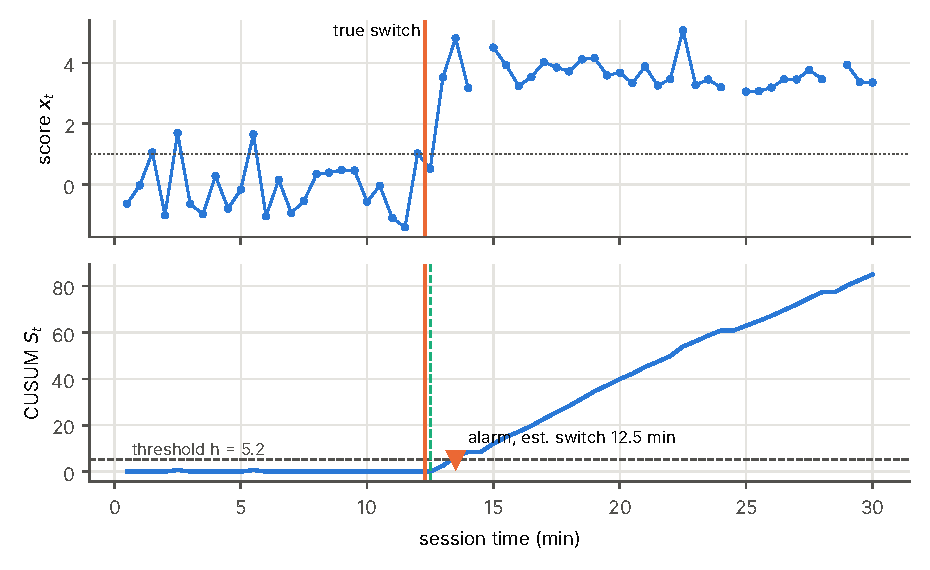
\includegraphics[width=0.85\linewidth]{cusum-trace-takeover}
  \caption{Identity channel on a synthetic session in which a speed-matched
    partner takes over. Top: standardised score per 30\,s window (gaps are
    inactive windows; dotted line $k$). Bottom: CUSUM statistic, threshold
    $h$, alarm and estimated switch time.}
  \label{fig:cusum-trace}
\end{figure}

\section{Baselines}
Scaled Manhattan \cite{killourhy2009comparing}, TypeNet-style
\cite{acien2022typenet}, Nosi IAT rhythm \cite{lueder2026nosi}. A Nosi-style
detector (the L-scale feature alone, same CUSUM) is already part of the
ablation; the other two are planned for the evaluation harness (phase 4).

\section{Synthetic-data pipeline}
Before Phase 2 data exists, the detector is built and tuned on simulated
sessions written in the editor's own event format, so the same code reads
simulated and real logs (\cref{fig:synthetic-evaluation}). Each simulated
typist has a stable habit profile: base digraph latency and spread,
personal digraph offsets, a hand-alternation speed-up, hold time, word-level
hesitations and think pauses before lines, typo and revision rates,
skeleton-first or linear code order, run frequency and how often they look
away. Every session adds day-to-day drift to each habit. The typists write
lab-style Python programs (with comments) until the session ends.

The five study conditions are simulated as: (A) honest composing; (B) a
different typist composes the whole session; (C) a second typist takes over
at a random minute after a 5--40\,s seat swap and continues the same code;
(D) the student switches to transcribing code from elsewhere (faster, more
uniform rhythm, fewer pauses and typos, glances away every 12--40
characters); (E) the student pastes chunks copied from elsewhere. Partners
for B and C are the typist nearest in base speed, a stand-in for the
study's grade-matched proxies; C is also run with a random partner.

\begin{figure}[ht]
  \centering
  \resizebox{\linewidth}{!}{\tikzfig{synthetic-evaluation}}
  \caption{Synthetic evaluation protocol.}
  \label{fig:synthetic-evaluation}
\end{figure}

Known simplifications: indentation is typed with Tab whereas the real
editor auto-indents and auto-closes brackets, mouse-driven editing is not
simulated, and simulated habits are independent draws, so real students
will be both more alike (shared curriculum, same keyboards) and more
variable (fatigue, difficulty of the task). The synthetic numbers show that
the pipeline works and how its settings trade off; they are not a claim
about real students.

\chapter{Study Design and Ethics}
\label{ch:study}

\section{Ethics and data protection}
\todo{Approval, consent, DPDP Act, EU AI Act design target.}

\section{Phase 0: survey and logger}
\todo{Months 1--2.}

\section{Phase 1: baseline labs}
\todo{60--80 volunteers, first four lab weeks.}

\section{Phase 2: staged conditions}
\begin{table}[ht]
  \centering
  \caption{Phase 2 staged conditions.}
  \label{tab:conditions}
  \begin{tabular}{@{}cl@{}}
    \toprule
    Condition & Description \\
    \midrule
    A & Honest session \\
    B & Full proxy (someone else writes the whole session) \\
    C & Takeover at a random minute \\
    D & Copying code out of another source \\
    E & Pasting \\
    \bottomrule
  \end{tabular}
\end{table}
\todo{Grade-matched proxies; counterbalancing; session length.}

\section{Phase 3: mock remote interview}
\todo{20--30 participants, own laptop.}

\section{Metrics}
\todo{Detection delay, false alarms per hour, AUC/EER, precision at
1/100 and 1/500 prevalence, per-subgroup error rates.}

\chapter{RQ1: Detecting a Mid-Session Switch}
\label{ch:rq1}
\section{Setup}
\todo{Data, splits, baselines compared.}
\section{Results}
\todo{Detection delay, false alarm rate, CUSUM traces from \texttt{graphs/}.}
\section{Ablations}
\todo{Feature-group and window-size ablations; full tables in
\cref{app:ablations}.}
\section{Summary}

\chapter{RQ2: Composing versus Transcribing}
\label{ch:rq2}
\section{Setup}
Replicate the Nosi scribing measure \cite{lueder2026nosi}: L-scale of
$\log(\mathrm{IAT})$ after removing pauses over 5 minutes and zero-length
intervals, classified with a linear SVM under leave-one-participant-out
cross-validation. Nosi's evidence is $N = 5$ expert authors on one task;
here it is tested on Phase 2 conditions A (honest) and D (copying out) with
the full participant pool.
\todo{Window length sweep (Nosi reports about 80\% at \SI{150}{\second});
comments-only typing as a known confound; per-student vs.\ population
thresholds.}
\section{Results}
\section{Summary}

\chapter{RQ3: Transfer to Remote Interviews}
\label{ch:rq3}
\section{Setup}
\todo{Lab baseline applied to own-laptop sessions; device shift.}
\section{Results}
\section{Summary}

\chapter{RQ4: Fairness and Precision at Realistic Rates}
\label{ch:rq4}
\section{Subgroup error rates}
\todo{Typing speed, keyboard layout, prior experience, gender, etc.\ from the
study's participant attributes (\texttt{students.csv} in the labels manifest).}

\subsection*{Synthetic test students (evaluation harness)}
Simulated people have no demographics, so the harness groups them by terciles
of their simulated habits: typing speed, rhythm variability and build style
(\cref{tab:harness-fairness,fig:harness-fairness}). Honest sessions flagged
range from 0\% (slow typists) to 12\% (steady rhythm) and matched takeovers
detected from 64\% (variable rhythm) to 100\% (slow and steady typists), but
with 10--23 students per group the intervals overlap. The variable-rhythm
group is the one to watch on real data: a typist whose own timing is
noisy gives the per-pair baseline wide spreads, so a different typist stands
out less. The machinery is in place; what it shows is that a
test set of 36 cannot establish or rule out a disparity of this size, which
argues for pooling subgroup analysis across all study phases or recruiting
towards the top of the planned 60--80.

% Generated by studentide.harness (synthetic:synth-v1-n120-s2026-b8-m30, test split, 36 students). Do not edit by hand.
\begin{table}[ht]
  \centering\small
  \caption{RQ4: error rates by subgroup for the thesis detector on the synthetic test students (95\% student-bootstrap intervals). Synthetic subgroups are terciles of the simulated habit profile; the study replaces them with recorded attributes.}
  \label{tab:harness-fairness}
  \resizebox{\linewidth}{!}{\begin{tabular}{@{}llrccc@{}}
    \toprule
    Attribute & Group & Students & Honest flagged & FA/h & Takeover detected \\
    \midrule
    build\_style & outline-first & 23 & 9\% {\scriptsize[2, 17]} & 0.39 {\scriptsize[0.04, 0.91]} & 61\% {\scriptsize[43, 78]} \\
     & top-down & 13 & 4\% {\scriptsize[0, 12]} & 0.08 {\scriptsize[0.00, 0.23]} & 69\% {\scriptsize[46, 92]} \\
    rhythm & medium & 12 & 8\% {\scriptsize[0, 21]} & 0.17 {\scriptsize[0.00, 0.42]} & 75\% {\scriptsize[50, 100]} \\
     & steady & 13 & 8\% {\scriptsize[0, 19]} & 0.54 {\scriptsize[0.00, 1.46]} & 54\% {\scriptsize[31, 85]} \\
     & variable & 11 & 5\% {\scriptsize[0, 14]} & 0.09 {\scriptsize[0.00, 0.27]} & 64\% {\scriptsize[36, 91]} \\
    typing\_speed & fast & 12 & 4\% {\scriptsize[0, 12]} & 0.17 {\scriptsize[0.00, 0.50]} & 75\% {\scriptsize[50, 100]} \\
     & medium & 14 & 14\% {\scriptsize[4, 29]} & 0.57 {\scriptsize[0.07, 1.42]} & 43\% {\scriptsize[21, 71]} \\
     & slow & 10 & 0\% {\scriptsize[0, 0]} & 0.00 {\scriptsize[0.00, 0.00]} & 80\% {\scriptsize[60, 100]} \\
    \bottomrule
  \end{tabular}}
\end{table}


\begin{figure}[ht]
  \centering
  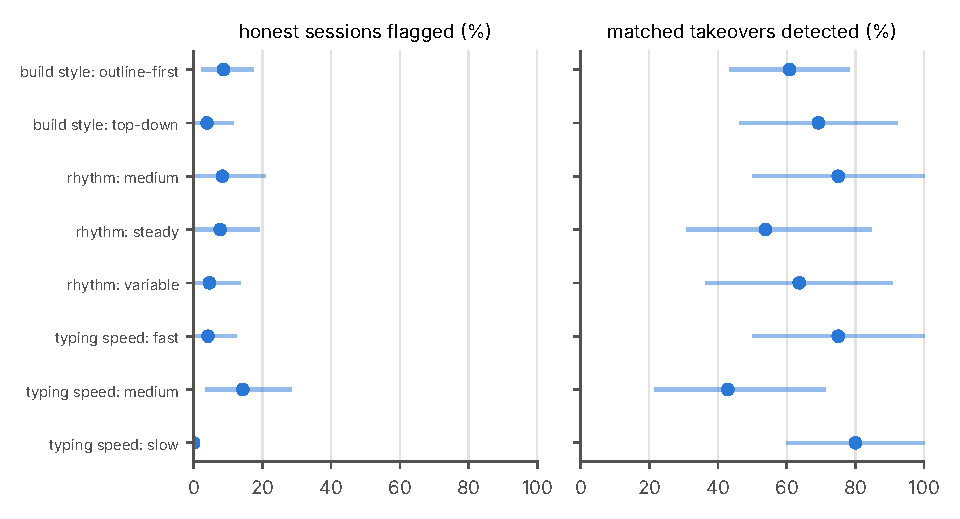
\includegraphics[width=\linewidth]{harness-fairness}
  \caption{Error rates by synthetic subgroup, 95\% student-bootstrap intervals.}
  \label{fig:harness-fairness}
\end{figure}

\section{Precision at low prevalence}
Precision $= \frac{\mathrm{TPR}\,\pi}{\mathrm{TPR}\,\pi + \mathrm{FPR}(1-\pi)}$
at $\pi = 1/100$ and $1/500$.

On the synthetic test students the thesis detector finds 92\% of non-honest
sessions and flags 7\% of honest ones (\cref{tab:harness-precision}). If 1 in 100
sessions involved a switch, about 12\% of flagged sessions would be real (95\%
interval 7--26\%); at 1 in 500, about 3\%. Put the other way, a teacher would
see 7.5 honest sessions flagged for every real one at 1 in 100, and 38 at 1 in
500. The key-pair channel raised detection but not the honest flag rate, so
precision barely moved (11\% before). The baselines, with lower TPR and similar
or higher FPR, are worse (4--6\% at 1 in 100). Lowering the operating point
helps but cannot fix this (\cref{fig:harness-precision}): at the lowest
calibrated false-alarm rate (3\% of honest sessions flagged, 81\% of
non-honest ones caught) precision at 1 in 100 reaches about 23\%.

This is the quantitative case for the design rule that a flag only ever starts
a conversation: at realistic rates most flags will be honest students, and any
use of the tool as evidence of misconduct would be wrong most of the time.

% Generated by studentide.harness (synthetic:synth-v1-n120-s2026-b8-m30, test split, 36 students). Do not edit by hand.
\begin{table}[ht]
  \centering\small
  \caption{RQ4: what a flag means at realistic cheating rates (synthetic test students, operating point of \cref{tab:harness-methods}). TPR: non-honest sessions with an alarm after the switch; FPR: honest sessions with any alarm. Precision $= \mathrm{TPR}\,\pi / (\mathrm{TPR}\,\pi + \mathrm{FPR}(1-\pi))$; honest flags per real one = $\mathrm{FPR}(1-\pi)/(\mathrm{TPR}\,\pi)$.}
  \label{tab:harness-precision}
  \resizebox{\linewidth}{!}{\begin{tabular}{@{}lccccrr@{}}
    \toprule
    Method & TPR & FPR & Prec.\ $\pi=1/100$ & Prec.\ $\pi=1/500$ & Honest per real (1/100) & (1/500) \\
    \midrule
    Two-channel CUSUM & 83\% & 7\% {\scriptsize[1, 12]} & 10.7\% {\scriptsize[6, 38]} & 2.3\% {\scriptsize[1, 11]} & 8.3 & 41.9 \\
    Scaled Manhattan & 53\% & 12\% & 4.1\% & 0.8\% & 23.2 & 117.0 \\
    TypeNet-style LSTM & 39\% & 10\% & 3.9\% & 0.8\% & 24.4 & 123.0 \\
    Nosi-style L-scale & 47\% & 7\% & 6.4\% & 1.3\% & 14.7 & 74.3 \\
    \bottomrule
  \end{tabular}}
\end{table}


\begin{figure}[ht]
  \centering
  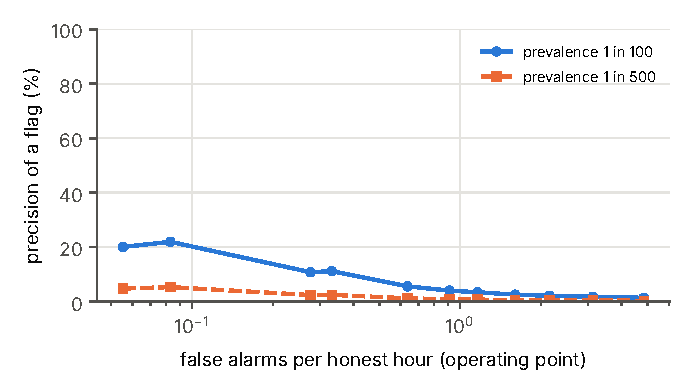
\includegraphics[width=0.65\linewidth]{harness-precision}
  \caption{Precision of a flag by operating point at two prevalences (thesis
    detector, synthetic test students).}
  \label{fig:harness-precision}
\end{figure}

\section{Summary}

\chapter{Discussion}
\label{ch:discussion}
\section{What the results mean for assessment}
\section{A flag is a conversation}
\todo{How teachers should use the timeline; harms of false flags.}
\section{Limitations}
\section{Threats to validity}

\chapter{Conclusion and Future Work}
\label{ch:conclusion}
\section{Conclusion}
\section{Future work}

\subsection{Sandbox Labs: a desktop client with local sandboxes}
\label{sec:desktop-client}
The pilot runs every student program on the college VM, which keeps the
runner simple but rules out a real terminal per student: sixty live Linux
shells on one VM would cost far more than today's short runs. A planned
\emph{Sandbox Labs} feature (Figure~\ref{fig:desktop-client}; full plan in
\texttt{thesis/plans/2026-10-30-desktop-client.md}) lets teachers set up their own
subjects and labs (an environment built from a checklist of tools rather than
a Dockerfile, assignments whose tests are checked against a reference
solution, and a library of labs teachers share with each other), each opened in a whole Linux instance per subject on the student's own
machine, with sudo, internet access for installing any tech stack (limited to
package registries in assessed labs), services and ports, a terminal, a file
tree, terminal editors such as vim, and our editor. Because a student is root
inside the instance, file, process and network capture runs in a sidecar
container they cannot stop, while key timing is captured in the app itself.
The client is an Electron app whose installer also sets up its own container
engine (rootless Podman in a small WSL2 distribution on Windows or a
lightweight VM on macOS), so students need no Docker installation; the
student's files are snapshotted to the server so work follows them to another
machine, including from a lab PC that cannot run the sandbox to one that can;
cloud instances exist only for teachers to preview a lab. Electron uses the same Chromium engine as the web editor, so
keystroke timestamps mean the same thing in both, which matters when a
baseline learned in the browser is compared with work done in the app. The
recorder is shared code, so the detector and review need no change for editor
work. The terminal becomes a new logged surface: key timing tagged by where it
was typed (editor, shell prompt or a terminal editor), commands, and files
changed outside the editor, shown like pastes. Because a student controls
their own machine, the client cannot be made tamper-proof; instead batches are
signed and hash-chained, submissions are graded on the server, and at
submission the server checks every file against the typing evidence behind it.

\begin{figure}[ht]
  \centering
  \resizebox{0.9\linewidth}{!}{\tikzfig{desktop-client}}
  \caption{Planned Sandbox Labs client: code runs in a local container (or a
  a cloud instance for teacher previews), while events, workspace snapshots and submissions go
  to the college server, where the detector and review are unchanged.}
  \label{fig:desktop-client}
\end{figure}

The teacher side of Sandbox Labs is built (Figure~\ref{fig:sandbox-teacher}).
Teachers create subjects without approval and give each an environment chosen
from a base and a checklist of tools; the server renders it to a Dockerfile
that a build service outside the college VM turns into an image. A lab is a
list of assignments, each with a statement, starter files, a run command, tests
(input/output pairs or a test command, some hidden) and a private reference
solution. Before publishing, a Check step runs the tests in the lab's real
environment: the reference solution must pass and the starter should fail.
Labs can be shared to a library as snapshots that colleagues copy into their
own subjects. A teacher can try any lab as a student in a short-lived cloud
instance with a terminal; these previews are capped (three seats, one per
teacher, an idle stop and an hour at most, never the open internet) so that
the VM cost the design moved to students' machines does not come back. Only a
separate service holds the Docker socket, and previews never create study
sessions.

\begin{figure}[ht]
  \centering
  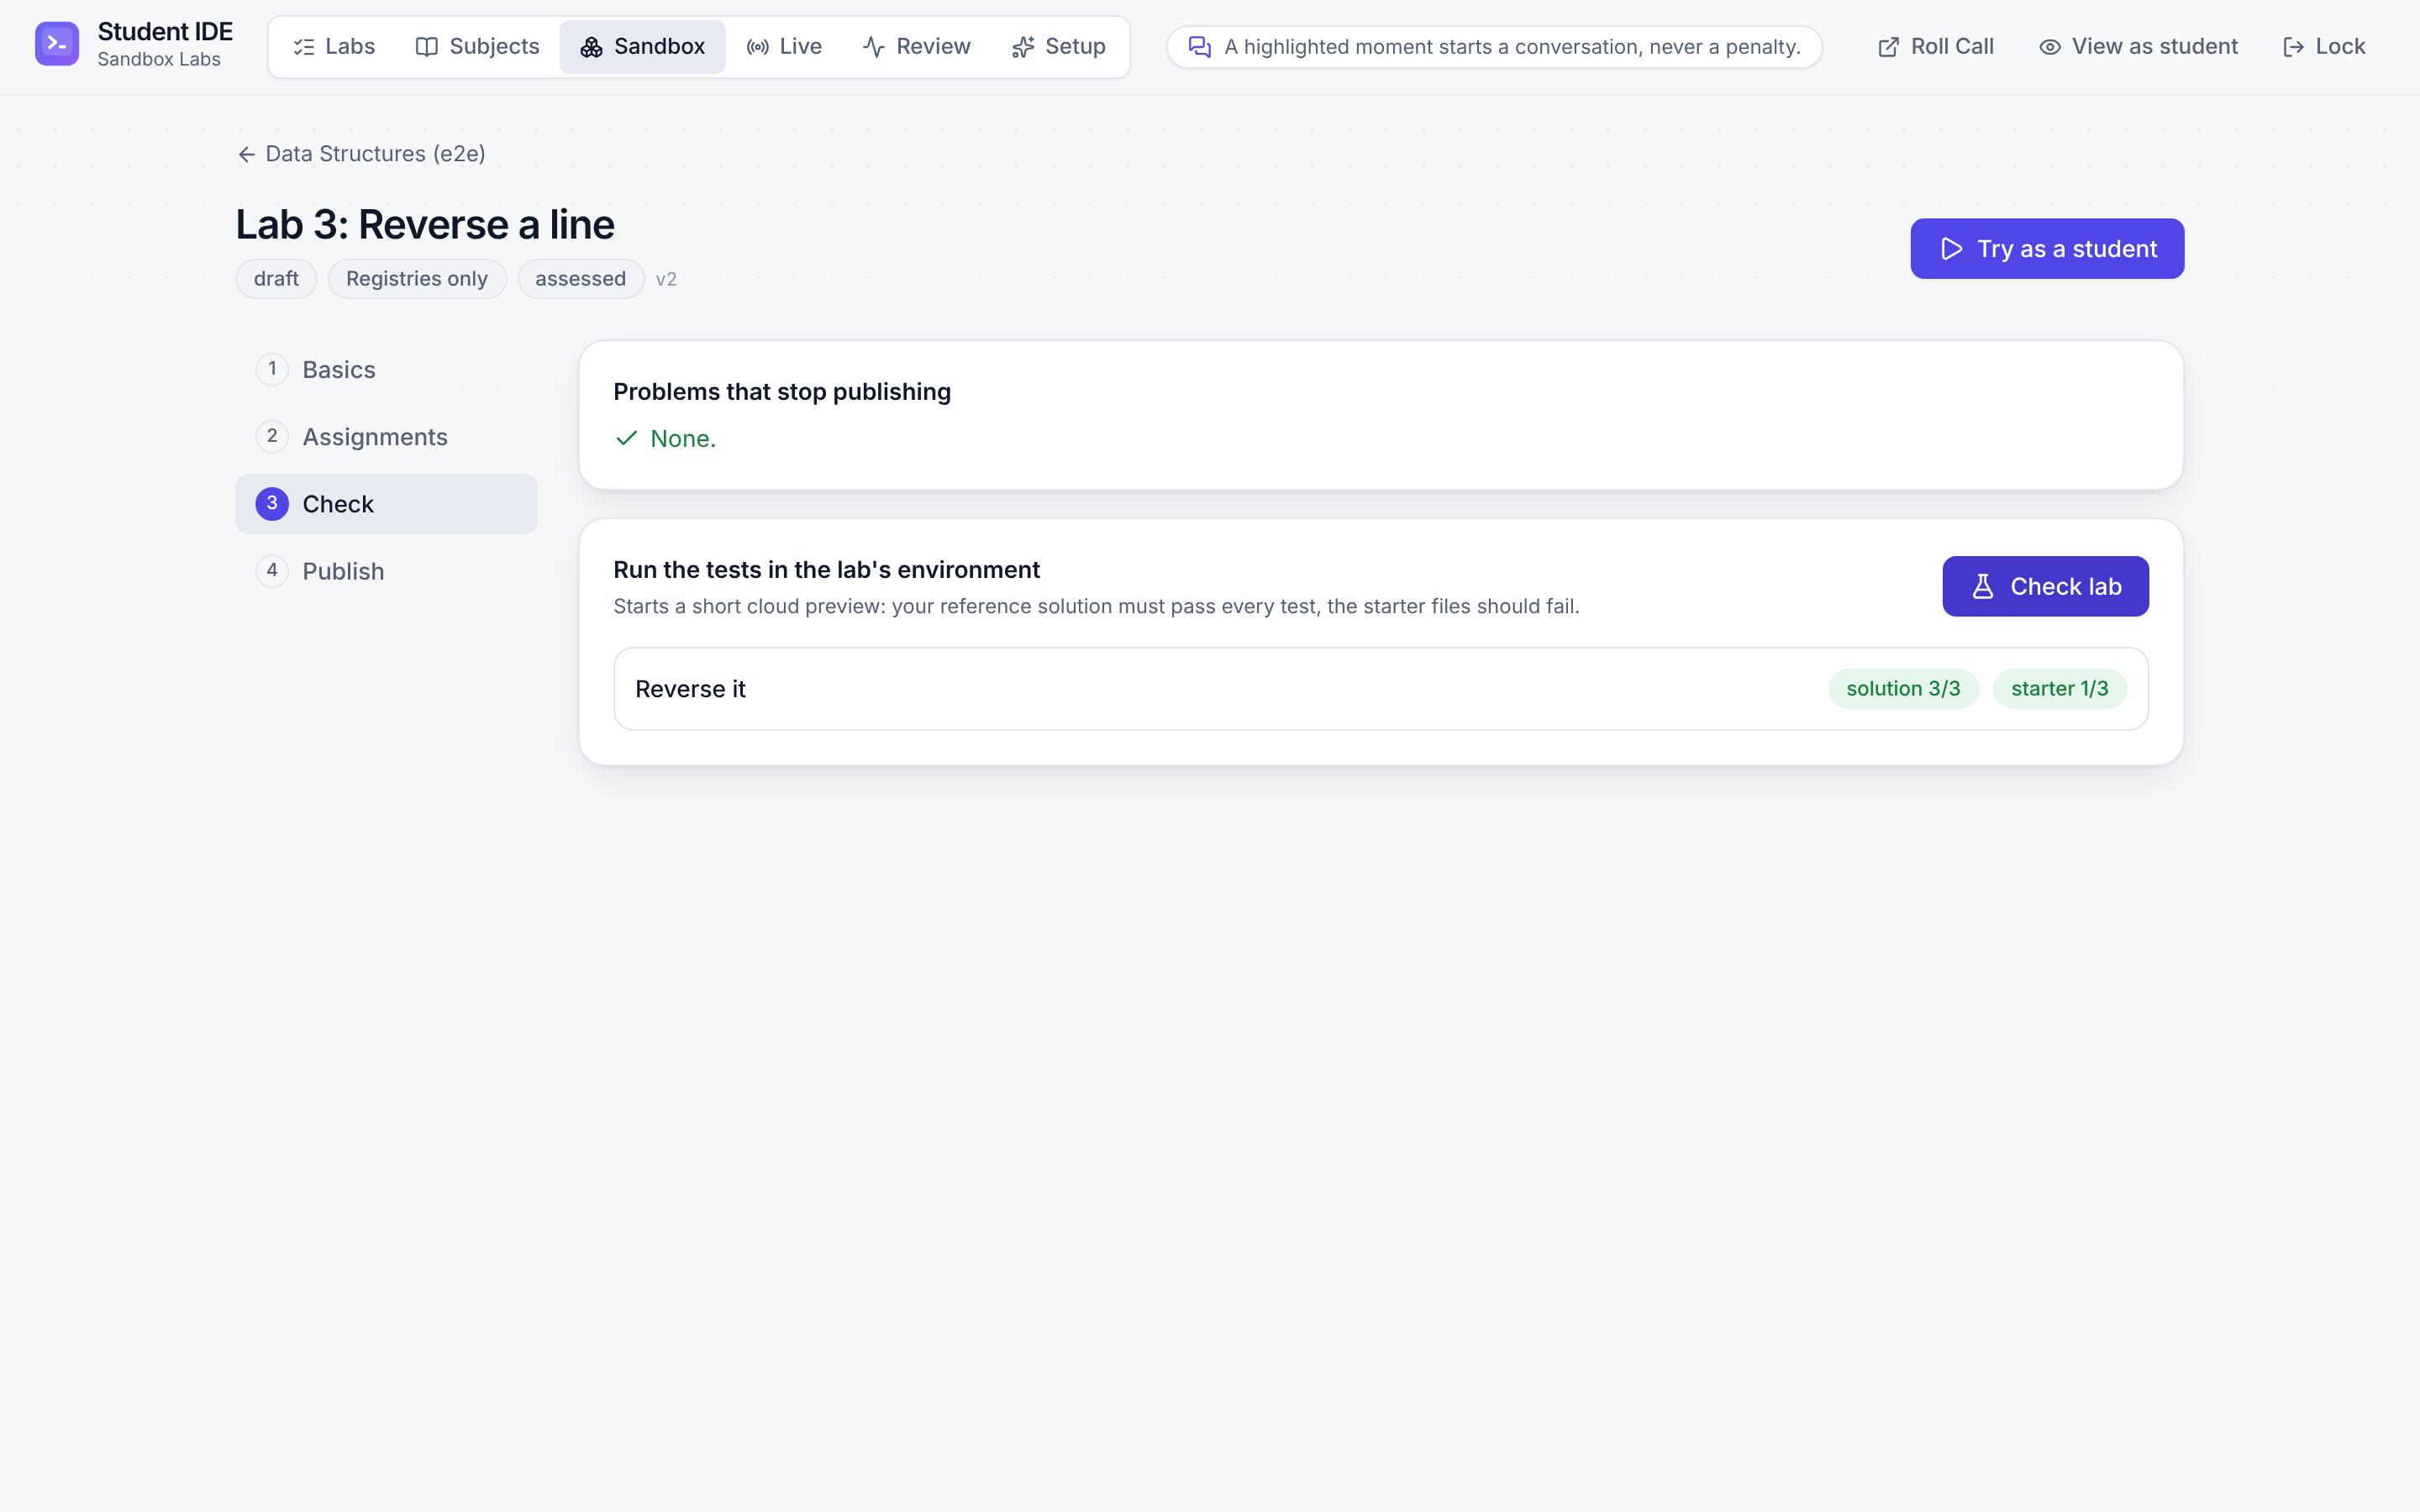
\includegraphics[width=0.49\linewidth]{sandbox/sandbox-light-05-check}\hfill
  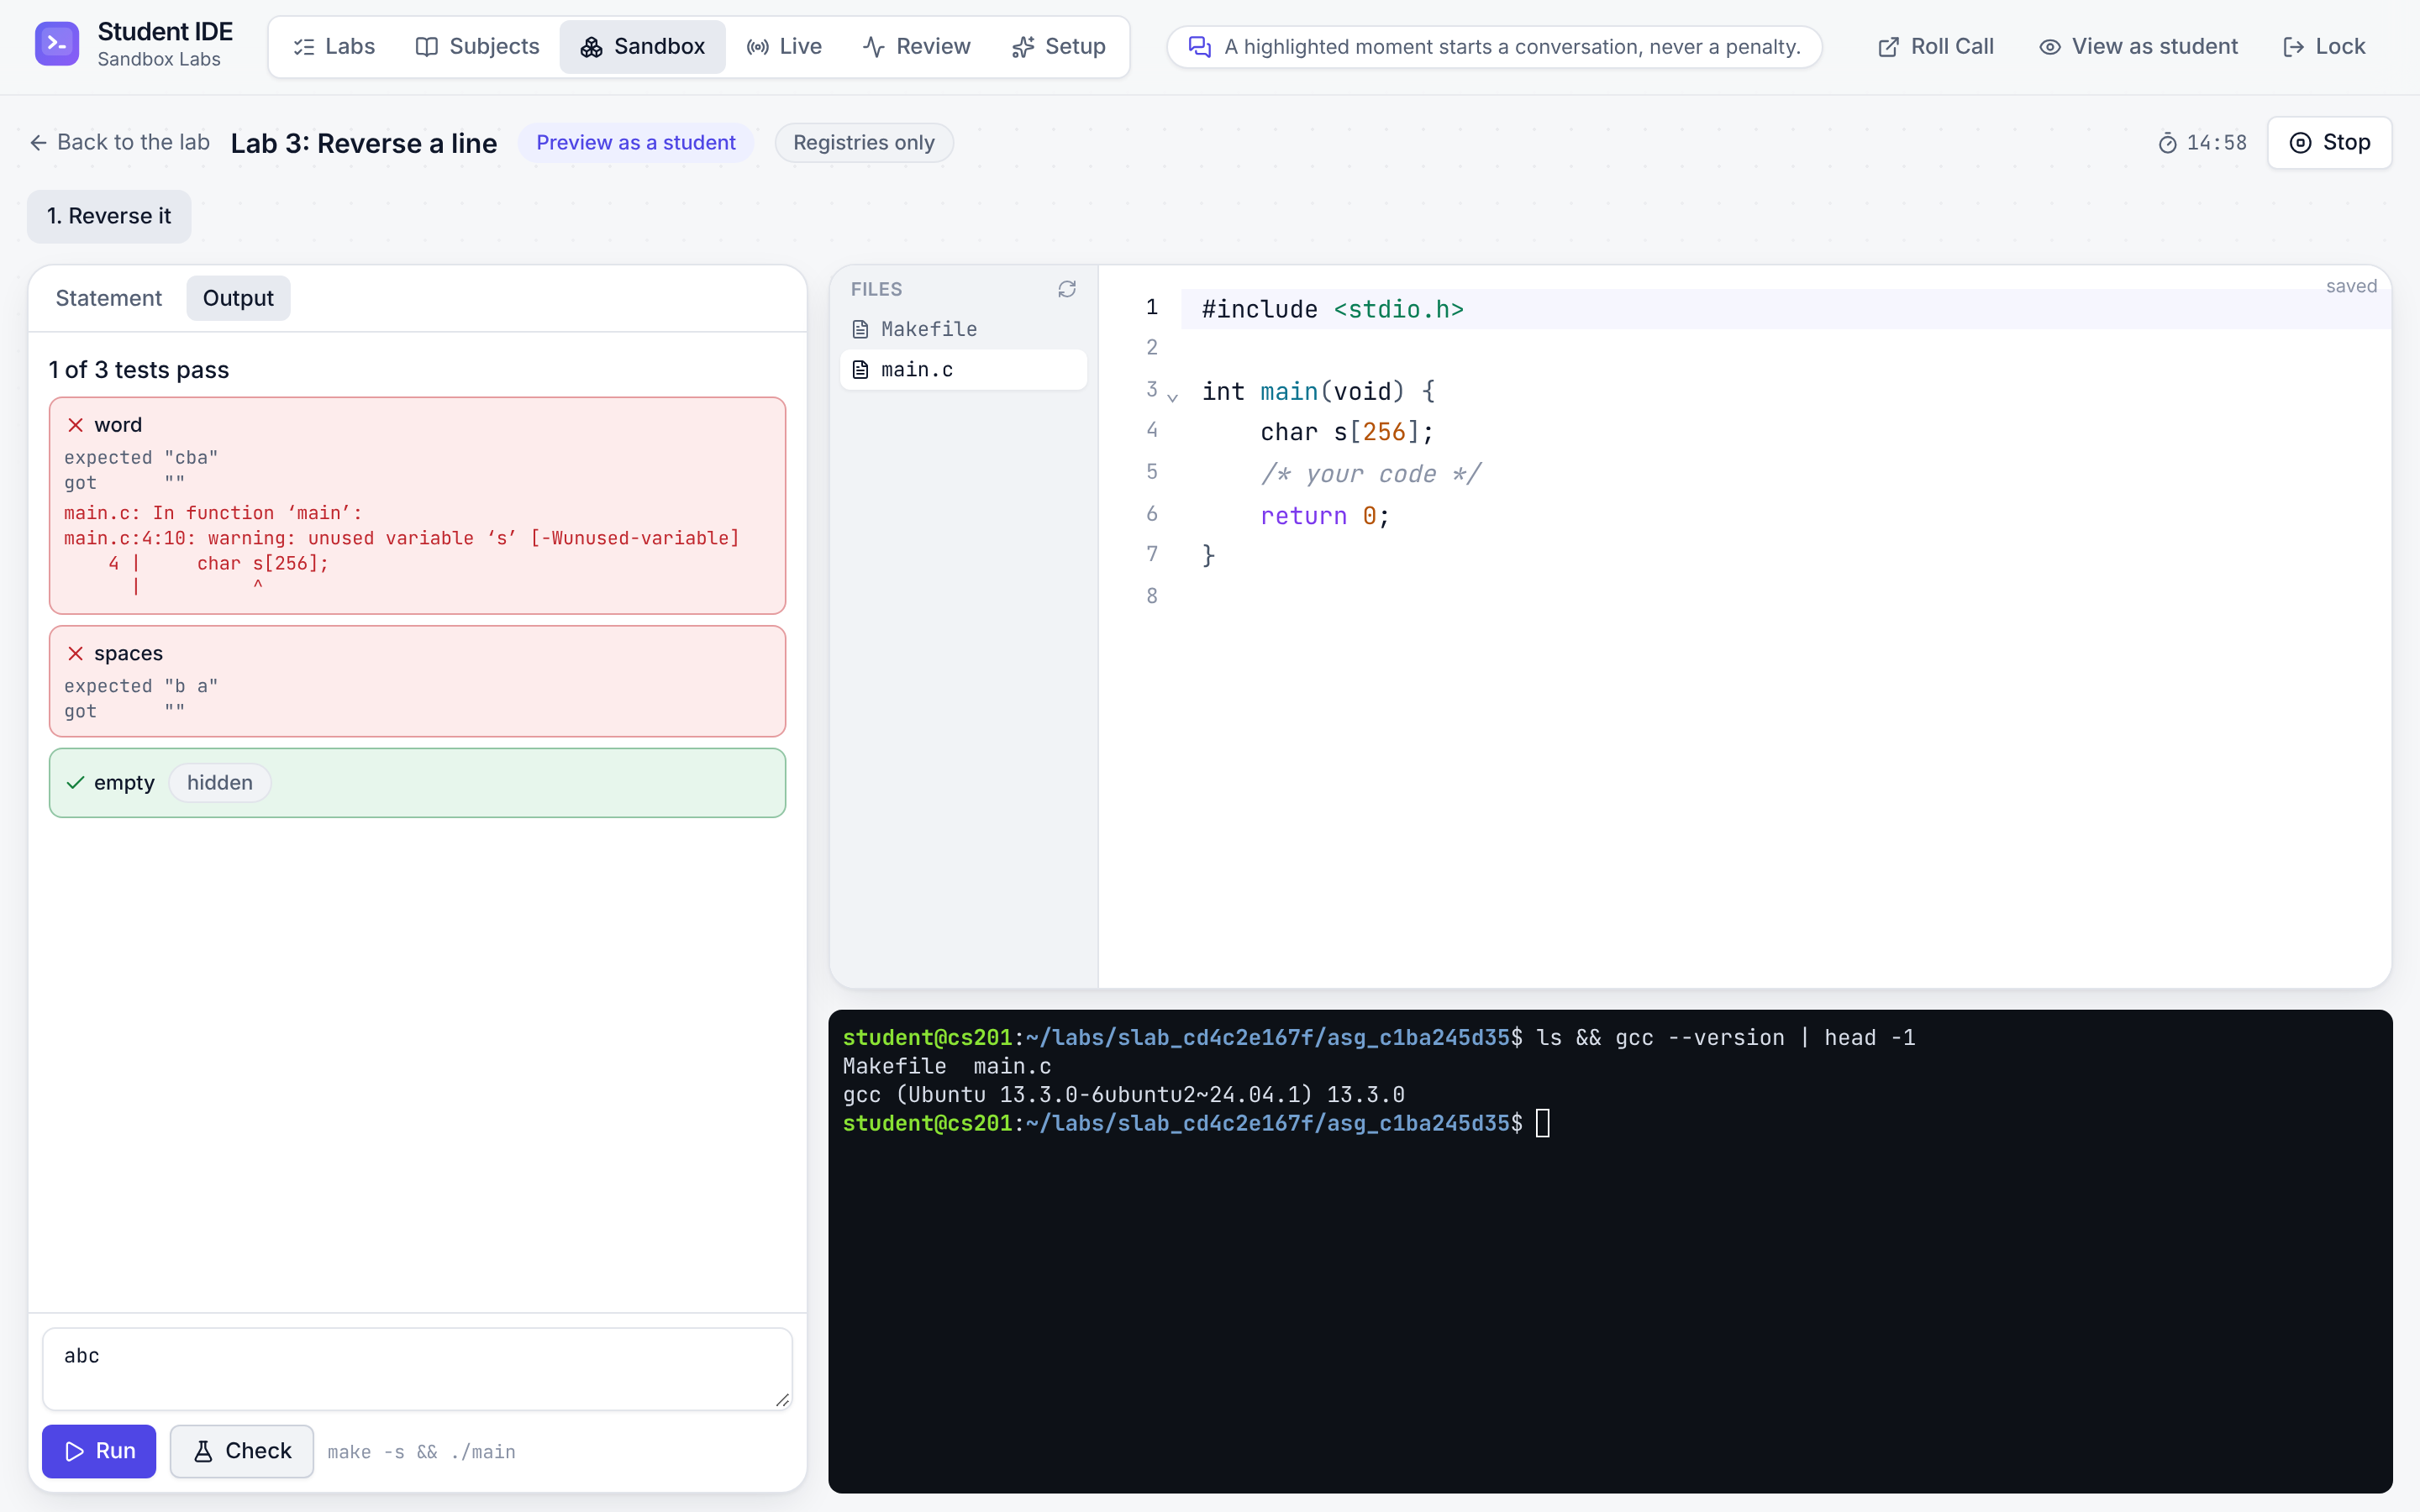
\includegraphics[width=0.49\linewidth]{sandbox/sandbox-light-06-try-as-student}
  \caption{Sandbox Labs, teacher side: the lab wizard's Check step (reference
  solution 3/3, starter 1/3) and ``Try as a student'' in a capped cloud
  preview with editor, terminal and the full test results.}
  \label{fig:sandbox-teacher}
\end{figure}


% ---------- Back matter ----------
\printbibliography[heading=bibintoc,title={References}]

\appendix
\chapter{Event Schema}
\label{app:schema}
\todo{Full schema of logged events, generated from the editor's code.}

\chapter{Ethics Approval and Consent Forms}
\label{app:ethics}
\todo{Approval letter, participant information sheet, consent form, survey.}

\chapter{Ablation Studies}
\label{app:ablations}
% One section per study. Put raw CSVs and the generated .tex table in
% ablations/<study-name>/ and \input the table here, e.g.
%   \input{ablations/window-size/table}
% Tables below are regenerated by
%   python -m studentide.detector.evaluate --typists 60 --seed 7 --thesis thesis/latex

\section{Window length (synthetic)}
% Generated by studentide.detector.evaluate (seed 7, 60 typists, 30-min sessions). Do not edit by hand.
\begin{table}[ht]
  \centering\small
  \caption{Window-length ablation on synthetic sessions. Window AUC/accuracy: one window,
    honest vs.\ typed by another person. Detection: CUSUM alarm after the switch, with $h$ set
    for $\le 0.2$ false alarms per hour on calibration typists (identity/process channel).
    Delay and switch-time error are medians.}
  \label{tab:ablation-window-length}
  \resizebox{\linewidth}{!}{\begin{tabular}{@{}rcccrrrcc@{}}
    \toprule
    $W$ (s) & Win.\ AUC & Win.\ acc. & $h$ & Takeover & Delay (s) & Switch err.\ (s) & Copying & FA/h \\
    \midrule
    10 & 0.85 & 0.78 & 4.5/23 & 72\% & 50 & 39 & 60\% & 0.60 \\
    20 & 0.86 & 0.79 & 6/9.75 & 78\% & 60 & 30 & 82\% & 0.87 \\
    30 & 0.88 & 0.80 & 5.25/16.5 & 72\% & 80 & 29 & 80\% & 0.42 \\
    60 & 0.90 & 0.83 & 11.75/15.75 & 60\% & 282 & 30 & 72\% & 0.12 \\
    90 & 0.91 & 0.84 & 7/9.5 & 72\% & 294 & 38 & 90\% & 0.27 \\
    120 & 0.92 & 0.85 & 7/7.5 & 62\% & 408 & 53 & 90\% & 0.25 \\
    150 & 0.92 & 0.85 & 5.25/5 & 68\% & 438 & 80 & 100\% & 0.30 \\
    \bottomrule
  \end{tabular}}
\end{table}


\section{Feature groups and detector design (synthetic)}
% Generated by studentide.detector.evaluate (seed 7, 60 typists, 30-min sessions). Do not edit by hand.
\begin{table}[ht]
  \centering\small
  \caption{Detector ablation on synthetic sessions ($W=30$\,s, $h$ recalibrated per row
    for $\le 0.2$ false alarms per hour). Share of sessions detected after the switch;
    delay is the median for matched-partner takeovers. Win.\ AUC is for the first channel listed.}
  \label{tab:ablation-feature-groups}
  \resizebox{\linewidth}{!}{\begin{tabular}{@{}lccccccr@{}}
    \toprule
    Configuration & Win.\ AUC & Proxy & Takeover & Copying & Paste & Delay (s) & FA/h \\
    \midrule
    Two channels (default) & 0.88 & 90\% & 72\% & 80\% & 78\% & 80 & 0.42 \\
    \quad without rhythm & 0.60 & 60\% & 38\% & 78\% & 75\% & 275 & 0.45 \\
    \quad without digraph & 0.90 & 88\% & 75\% & 80\% & 78\% & 117 & 0.35 \\
    \quad without pauses & 0.88 & 90\% & 72\% & 82\% & 78\% & 80 & 0.40 \\
    \quad without revision & 0.88 & 90\% & 72\% & 95\% & 85\% & 80 & 0.40 \\
    \quad without build order & 0.88 & 85\% & 80\% & 95\% & 92\% & 96 & 0.47 \\
    \quad without runs & 0.88 & 90\% & 72\% & 80\% & 75\% & 80 & 0.40 \\
    \quad without focus & 0.88 & 90\% & 72\% & 8\% & 45\% & 80 & 0.42 \\
    \quad without paste & 0.88 & 90\% & 72\% & 80\% & 32\% & 80 & 0.42 \\
    Identity channel only & 0.88 & 80\% & 75\% & 10\% & 15\% & 69 & 0.52 \\
    Process channel only & 0.62 & 38\% & 20\% & 85\% & 88\% & 491 & 0.20 \\
    Old build order (edit position, caret jumps) & 0.88 & 88\% & 75\% & 50\% & 82\% & 86 & 0.42 \\
    Identity channel with $k=0.5$ & 0.88 & 92\% & 72\% & 80\% & 80\% & 188 & 0.32 \\
    One channel, all features, equal weights & 0.79 & 85\% & 60\% & 80\% & 90\% & 304 & 0.22 \\
    One channel, all features, ICC weights & 0.88 & 90\% & 70\% & 10\% & 10\% & 185 & 0.27 \\
    Nosi-style: L-scale of log IKI only & 0.65 & 40\% & 18\% & 42\% & 0\% & 566 & 0.00 \\
    Comments mixed into code & 0.89 & 88\% & 72\% & 80\% & 80\% & 92 & 0.37 \\
    \bottomrule
  \end{tabular}}
\end{table}


\section{Template}
% Template ablation table. Copy this folder for a real study, keep the raw
% results next to it as results.csv, and record the run in a brain entry.
\begin{table}[ht]
  \centering
  \caption{Template: feature-group ablation for switch detection
    (placeholder, no real numbers yet).}
  \label{tab:ablation-example}
  \begin{tabular}{@{}lccc@{}}
    \toprule
    Features removed & Detection delay (s) & False alarms / h & AUC \\
    \midrule
    None (full model)  & -- & -- & -- \\
    Digraph latency    & -- & -- & -- \\
    Pauses             & -- & -- & -- \\
    AST build order    & -- & -- & -- \\
    \bottomrule
  \end{tabular}
\end{table}



\end{document}
